% Moire Fields. Build: tectonic -X compile paper.tex --outdir build
\documentclass[acmtog, nonacm]{acmart}

\usepackage{amsmath}
% acmart's text font already defines a blackboard k; amssymb wants to as well.
\let\Bbbk\relax
\usepackage{amssymb}
\usepackage{amsthm}
\usepackage{booktabs}
\usepackage{graphicx}
\usepackage{subcaption}
\usepackage{tikz}
\usepackage{pgfplots}
\usepackage{pgfplotstable}
\usepackage{algorithm}
\usepackage{algpseudocode}

\pgfplotsset{compat=1.18}
\usetikzlibrary{calc, arrows.meta, decorations.pathreplacing, patterns, positioning, fit}

\definecolor{ink}{HTML}{15181C}
\definecolor{accent}{HTML}{C81E5A}
\definecolor{cool}{HTML}{1B6CA8}
\definecolor{warm}{HTML}{D4761A}
\definecolor{soft}{HTML}{8A94A0}
\definecolor{paperbg}{HTML}{F7F7F5}

\pgfplotsset{
  paperaxis/.style={
    width=\linewidth, height=4.4cm,
    tick align=outside, tick pos=left,
    axis line style={gray!60},
    grid=major, grid style={gray!18, very thin},
    label style={font=\small}, tick label style={font=\footnotesize},
    legend style={font=\footnotesize, draw=gray!40, fill=white, fill opacity=0.92,
                  text opacity=1, inner sep=2pt, row sep=-1pt},
  },
  smallaxis/.style={paperaxis, height=3.6cm},
}

% Figure captions read as standalone paragraphs, so they get a lead-in.
\newcommand{\figlead}[1]{\textbf{#1}\ }

% Two narrow columns full of monospaced identifiers and inline mathematics leave
% TeX few break points; a little emergency stretch is cheaper than a slug of
% overfull lines.
\setlength{\emergencystretch}{1.2em}
% A slash inside a monospaced path, with a break opportunity after it.
\newcommand{\pslash}{\discretionary{/}{}{/}}

% Reference entries carry unbreakable DOIs, so a few lines cannot be justified at
% all. Be sloppy there rather than in the body, where the stretch would show.
\AtBeginEnvironment{thebibliography}{\sloppy}

% Labels centred under the panels of a strip figure. The strips are assembled as
% single images by tools/lib/render.mjs, so the geometry has to be restated here:
% #1 is the panel width and #2 the gutter, both as fractions of the image width,
% and #3 is a comma list of labels.
% The row is one unbreakable box: the fractions sum to the full width by
% construction, so any line breaking at all would scatter the labels.
\newcommand{\panelrow}[3]{%
  \par\nointerlineskip\vskip 2.5pt%
  \noindent\makebox[\linewidth][l]{\footnotesize
    \foreach \panellabel [count=\panelno] in {#3}{%
      \ifnum\panelno>1\hspace{#2\linewidth}\fi
      \makebox[#1\linewidth][c]{\panellabel}%
    }\hss}%
  \par
}

\theoremstyle{plain}
\newtheorem{theorem}{Theorem}
\newtheorem{proposition}[theorem]{Proposition}
\newtheorem{lemma}[theorem]{Lemma}
\newtheorem{corollary}[theorem]{Corollary}
\theoremstyle{definition}
\newtheorem{definition}[theorem]{Definition}
\newtheorem{remark}[theorem]{Remark}

\newcommand{\R}{\mathbb{R}}
\newcommand{\N}{\mathbb{N}}
\newcommand{\Z}{\mathbb{Z}}
\newcommand{\Rot}[1]{\mathbf{R}_{#1}}
\newcommand{\rad}{\rho}
\newcommand{\idx}{\phi}
\newcommand{\ph}{\psi}
\newcommand{\het}{\eta}
\newcommand{\Moire}{\textsc{Moir\'e}}
\newcommand{\ours}{\textsc{Window}}
\newcommand{\sweep}{\textsc{Sweep}}
\newcommand{\loose}{\textsc{Loose}}

% GENERATED by paper/tools/numbers.mjs -- do not edit by hand.
% Every number the prose quotes, in one place, so text and data cannot drift.

% ---- src/types/moire.ts : what the Studio offers
\newcommand{\fieldCount}{six}
\newcommand{\patternCount}{thirteen}
\newcommand{\envTaps}{24}

% ---- data/fringe.json : the fringe law
\newcommand{\fringeScenes}{12}
\newcommand{\fringeSamples}{107{,}691}
\newcommand{\fringeMeanErr}{0.0034}
\newcommand{\fringeWorstP}{0.073}
\newcommand{\fringeLight}{0.036}
\newcommand{\fringeDark}{0.416}
\newcommand{\fringeRegime}{1/4}

% ---- data/lawatlas.json : admitted fraction per panel
\newcommand{\atlasCombs}{100.0}
\newcommand{\atlasCircleLines}{39.1}
\newcommand{\atlasHex}{93.5}
\newcommand{\atlasCircles}{21.7}
\newcommand{\atlasControl}{0.0}

% ---- data/gradient.json : the missing gradient divide
\newcommand{\gradWorstWave}{25.2}
\newcommand{\gradWorstHyp}{14.8}
\newcommand{\gradWorstSpiral}{7.3}
\newcommand{\gradWorstParab}{224}
\newcommand{\gradWaveFrame}{61}
\newcommand{\gradHypFrame}{66}
\newcommand{\gradParabFrame}{98}
\newcommand{\gradSpiralFrame}{0}

% ---- data/gpu.json : 1200x800 = 0.96 Mpixel, one full-screen layer
\newcommand{\gpuSpeedLo}{11}
\newcommand{\gpuSpeedHi}{37}
\newcommand{\gpuTriRotOne}{14.4}
\newcommand{\gpuTriRotOneNew}{0.39}
\newcommand{\gpuTriRotOffOut}{27.9}
\newcommand{\gpuTriRotOffOutNew}{1.64}
\newcommand{\gpuSquareOld}{0.92}
\newcommand{\gpuSquareClosed}{0.20}
\newcommand{\gpuSquareClosedGain}{4.7}
\newcommand{\gpuAdapter}{metal-3}

% ---- data/gpu.json : interpreting a field expression against unrolling it
\newcommand{\interpPerOp}{0.103}
\newcommand{\interpLo}{0.63}
\newcommand{\interpHi}{6.9}
\newcommand{\interpHiOps}{67}
\newcommand{\unrolledLo}{0.0043}
\newcommand{\unrolledCeil}{0.054}
\newcommand{\fieldBaseline}{0.0071}
\newcommand{\fieldEmptyCost}{0.044}
\newcommand{\fieldEmptyGain}{6}
\newcommand{\fieldOpsLo}{6}
\newcommand{\fieldOpsHi}{67}
\newcommand{\fieldStmtHi}{73}
\newcommand{\fieldTwinWorst}{4{\times}10^{-5}}
\newcommand{\fieldGainLo}{40}
\newcommand{\fieldGainHi}{265}

% ---- data/cost.json : CPU metric evaluations per pixel, mean
\newcommand{\costScenes}{7}
\newcommand{\costSweepLo}{180}
\newcommand{\costSweepHi}{361}
\newcommand{\costOursLo}{7.5}
\newcommand{\costOursHi}{11.1}
\newcommand{\costVsSweepLo}{18}
\newcommand{\costVsSweepHi}{33}
\newcommand{\costVsRefLo}{1.7}
\newcommand{\costVsRefHi}{9.4}

% ---- data/artifacts.json
\newcommand{\artHolesSweepDiff}{8.6}
\newcommand{\artHolesSweepEv}{1100}
\newcommand{\artHolesOursEv}{72}
\newcommand{\artHolesSaving}{15}
\newcommand{\artDriftLooseDiff}{38.3}
\newcommand{\artDriftRefInk}{0.459}
\newcommand{\artDriftLooseInk}{0.152}
\newcommand{\artAnchorEv}{33}
\newcommand{\artAnchorRefInk}{0.489}
\newcommand{\artAnchorLatticeInk}{0.216}
\newcommand{\artAnchorPixelInk}{0.216}

% ---- data/fidelity.json : the sweep against the exhaustive reference
\newcommand{\fidSettings}{2{,}401}
\newcommand{\fidLegible}{1{,}534}
\newcommand{\fidSweepHoles}{160}
\newcommand{\fidSweepWorst}{32.9}
\newcommand{\fidSweepLegibleHoles}{3}
\newcommand{\fidSweepLegibleWorst}{4.2}
\newcommand{\fidSweepEnvelopeHoles}{41}
\newcommand{\fidSweepEnvelopeWorst}{29.6}
\newcommand{\fidLooseHoles}{46}
\newcommand{\fidLooseWorst}{48.3}
\newcommand{\fidLooseEnvelopeHoles}{13}
\newcommand{\fidOursHoles}{146}
\newcommand{\fidOursWorst}{13.8}

% ---- data/saturation.json : the interval-width sweep
\newcommand{\satSettings}{55{,}692}
\newcommand{\satFitting}{45{,}774}
\newcommand{\satFittingPct}{82}
\newcommand{\satStrided}{9{,}918}
\newcommand{\satWidestFitting}{1022}
\newcommand{\satMedianInk}{0.89}
\newcommand{\satStridedLegible}{1{,}472}
\newcommand{\satStridedLegiblePct}{2.6}
\newcommand{\satBudget}{1{,}024}
\newcommand{\satDriftRatioHi}{4.2}

% ---- data/degenerate.json : strided band against a deep scan
\newcommand{\degChecked}{534}
\newcommand{\degWithDrop}{217}
\newcommand{\degWorst}{48.8}
\newcommand{\degMean}{4.6}
\newcommand{\degLegible}{298}
\newcommand{\degLegibleWorst}{28.7}

% ---- data/residual.json : the worked pixel of the window figure
\newcommand{\figNaive}{49}
\newcommand{\figTrue}{41}
\newcommand{\figGap}{8}
\newcommand{\figLo}{22}
\newcommand{\figHi}{56}
\newcommand{\figSpan}{35}
\newcommand{\figEvals}{9}
\newcommand{\figGuard}{10.5}
\newcommand{\figSpacing}{14}

% ---- data/window.json : the interval checked against a brute-force argmin
\newcommand{\winChecks}{13{,}458}
\newcommand{\winViolations}{0}

% ---- data/ablation.json : one mechanism removed, time relative to full
\newcommand{\ablSkipLo}{2.1}
\newcommand{\ablSkipHi}{3.3}
\newcommand{\ablClosedMarginal}{90.3}
\newcommand{\ablCostLo}{8}
\newcommand{\ablCostHi}{19}
\newcommand{\ablMpixel}{3.84}

% ---- data/zoom.json : zoom stability
\newcommand{\zoomDecades}{1.2}
\newcommand{\zoomRefSamples}{36}
\newcommand{\zoomCoarsestPeriod}{1.5}
\newcommand{\zoomFloorNoise}{0.046}
\newcommand{\zoomNoFloorNoise}{0.115}
\newcommand{\zoomValueNoise}{0.118}
\newcommand{\zoomFloorNoiseCoarse}{0.002}
\newcommand{\zoomNoFloorNoiseCoarse}{0.115}
\newcommand{\zoomNoiseRatio}{77}
\newcommand{\zoomFloorInkGain}{0.61}
\newcommand{\zoomValueBias}{0.004}

% ---- data/contour.json : moire as a contouring primitive
\newcommand{\contourCarrier}{5}
\newcommand{\contourDetune}{5.5556}
\newcommand{\contourCtlGap}{50}
\newcommand{\contourFloor}{0.22}
\newcommand{\contourFloorP}{0.61}
\newcommand{\contourBestErr}{0.23}
\newcommand{\contourWorstErr}{0.58}
\newcommand{\contourAtFloor}{three}
\newcommand{\contourAtFloorErr}{0.25}
\newcommand{\contourFieldCount}{six}
\newcommand{\contourWorstP}{2.62}
\newcommand{\contourProbes}{63{,}904}
\newcommand{\contourFinest}{8.14}
\newcommand{\contourDipoleResolved}{86}
\newcommand{\contourDipoleFinest}{8.14}


\begin{document}

\title{Moir\'e Fields}
\subtitle{Interference as a scalar field, and a tool for drawing with it}

\author{Neo Mohsenvand}
% obeypunctuation stops acmart appending a comma after the institution; the class
% insists on a city and a country, and there is no true value for either, so both
% get a space rather than an invented place.
\affiliation[obeypunctuation=true]{\institution{Independent}\city{\ }\country{\ }}
% The class footnotes an address block built from the affiliation, which for a
% single unaffiliated author is just the byline again.
\authorsaddresses{}

\begin{abstract}
Moir\'e is the oldest computational image: two dense families of curves, and a
third pattern that belongs to neither. Graphics treats it as an aliasing artifact
to filter away, or as a printed pair of gratings solved offline and slid by hand;
neither lets an artist hold a moir\'e and move it. We represent a layer instead
as two scalar fields --- an index field naming the nearest member of a curve
family, fractionally, and a distance field to it --- so superposition composites
fields rather than pixels and the pattern has no resolution. In this model the
fringes of a superposition are exactly the unit level sets of the index-field
difference, with a saturating tent profile and a per-pixel validity criterion; no
periodicity is required. The hard case is a family whose members each carry their
own rigid motion: its index field has no closed form, and the nearest member must
be searched for. The support function of the generating shape supplies a provably
sufficient search interval, a Lipschitz skip rule, and an exact closed form for
translated polygons --- $\gpuSpeedLo$--$\gpuSpeedHi\times$ faster than the fixed
enumeration it replaces, at equal or better fidelity. We present \Moire{}, a
browser studio built on the model, and show that choosing the index difference
turns a moir\'e into a live contour plot of any authored field, within
$\contourWorstErr$\,px of the true level sets.
\end{abstract}

\begin{CCSXML}
<ccs2012>
<concept><concept_id>10010147.10010371.10010372</concept_id><concept_desc>Computing methodologies~Rendering</concept_desc><concept_significance>500</concept_significance></concept>
<concept><concept_id>10010147.10010371.10010396</concept_id><concept_desc>Computing methodologies~Shape modeling</concept_desc><concept_significance>300</concept_significance></concept>
<concept><concept_id>10003120.10003121.10003124</concept_id><concept_desc>Human-centered computing~Interaction techniques</concept_desc><concept_significance>100</concept_significance></concept>
</ccs2012>
\end{CCSXML}

\ccsdesc[500]{Computing methodologies~Rendering}
\ccsdesc[300]{Computing methodologies~Shape modeling}
\ccsdesc[100]{Human-centered computing~Interaction techniques}

\keywords{moir\'e, interference, distance fields, support functions, procedural
patterns, interactive authoring, {GPU} rendering}

\begin{teaserfigure}
  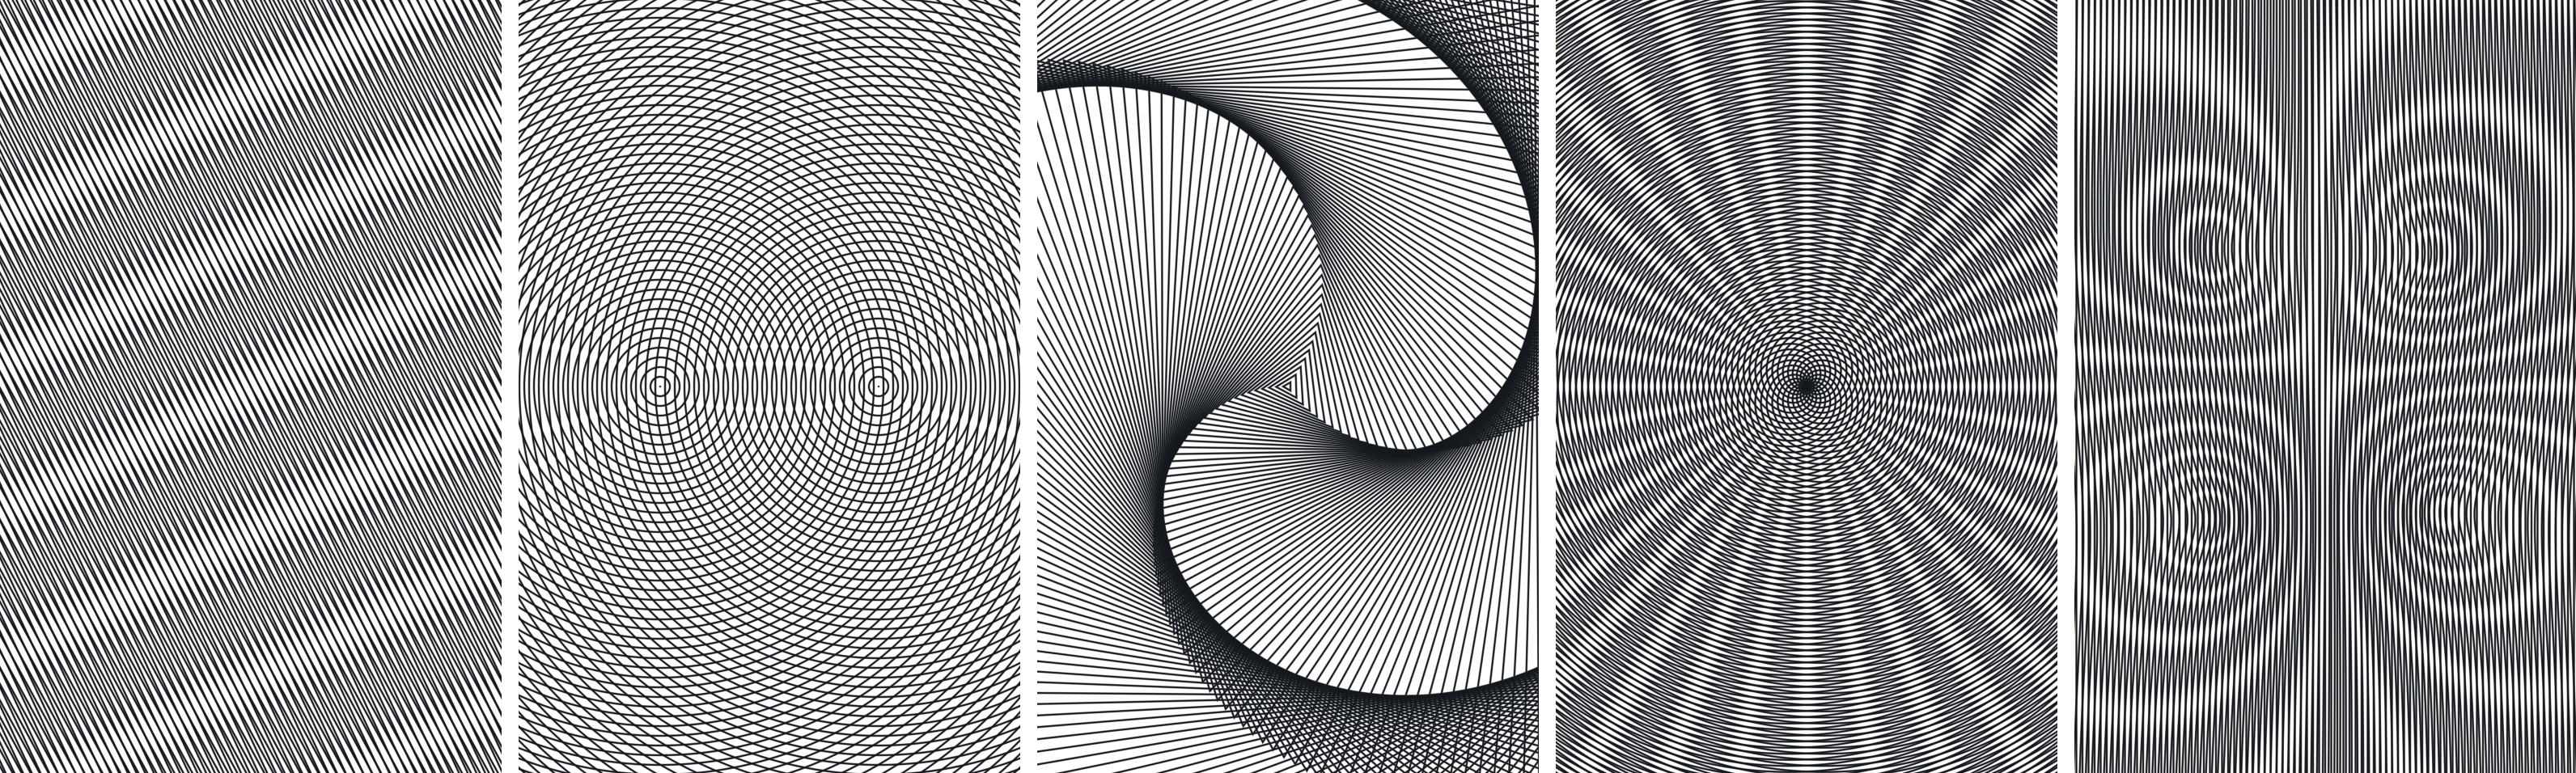
\includegraphics[width=\linewidth]{figures/teaser.png}
  \panelrow{0.19470}{0.00662}{%
    (1) two combs,
    (2) two ring families,
    (3) one walking family,
    (4) mirrored spirals,
    (5) a chosen field}
  \Description{Five tall panels in a row, each a dense hairline drawing in
  near-black over white. Left to right: two overlapping combs of parallel lines
  crossed at a shallow angle, producing three broad pale diagonal bands; two sets
  of concentric rings about centres left and right of middle, producing nested
  pale hyperbolic channels; a single family of concentric triangles each rotated
  and shifted from the last, producing a three-armed pinwheel whose envelope
  crosses itself in dark crosshatched lobes; two Archimedean spirals mirrored
  about the horizontal axis, producing a starburst of about thirty-six pale rays;
  and a field of curved bands looping around four centres, the streamlines of a
  four-vortex flow.}
  \caption{\figlead{No rasters anywhere.} Five superpositions, ordered left to
  right by how much the classical theory of moir\'e can say about them. Every one
  is a pair of scalar fields evaluated once per pixel --- each family answers
  ``how far to your nearest member, and which one is it'' --- so each is the same
  picture at any zoom and every number in it is a live slider. Both families in a
  panel are drawn in one ink, because the fringe law is a statement about total
  coverage: the pale sets \emph{are} the fringes.
  \textbf{(1)}~Two line combs three and a half degrees apart: Rayleigh's
  picture~\cite{Rayleigh1874Gratings}, and the only one spectral theory handles
  exactly. \textbf{(2)}~Rings about two centres; the
  fringes are the confocal hyperbolae where the two radii differ by a whole
  spacing, which is Theorem~\ref{thm:fringe} in its simplest instance.
  \textbf{(3)}~A \emph{single} family in which member $n$ is turned by $n\theta$
  and pushed by $n\delta$. It has no global index field and no partner layer: it
  interferes with itself, and finding the nearest member is the search problem of
  \S\ref{sec:inverse}. \textbf{(4)}~An Archimedean spiral against its own
  reflection --- not periodic, not a transform of anything periodic, and so
  outside Fourier moir\'e theory, but still a difference of two closed-form
  indices, and that difference is $-M\arg p/\pi$: hence exactly $2M=36$ rays.
  \textbf{(5)}~The same construction run backwards: the index difference
  is \emph{chosen}, here to be the stream function of four point vortices, so the
  fringes are streamlines of the flow (\S\ref{sec:beyond}). No curve was traced and
  no trajectory integrated --- it is one setting on an ordinary layer.
  Settings in the supplemental material (\S S4).}
  \label{fig:teaser}
\end{teaserfigure}

\maketitle

\section{Introduction}
\label{sec:intro}

Draw a comb of parallel lines on tracing paper, draw another, lay one over the
other and turn it a few degrees. A third pattern appears: broad, slow bands that
belong to neither sheet, made of ink already on the page and rearranged by
nothing but the small difference between two nearly identical structures.
Moir\'e has been a precision instrument since Rayleigh judged ruled gratings by
the fringes they made against their own copies~\cite{Rayleigh1874Gratings} and
Righi read grating displacement from fringe
motion~\cite{Righi1887Sovrapposizione}. It became an artistic medium in the
1960s~\cite{Oster1963Moire, Oster1965Optical, Seitz1965Responsive}, and artists
have built patterns for it since, by hand~\cite{Watkins1982Kinetic} and by the
plate~\cite{Nicolai2010Index}; it acquired a complete Fourier
theory~\cite{Amidror2009Theory}; it grounded a security-printing
discipline~\cite{Hersch2004Band, Chosson2014Beating}; and it reappeared at the
nanoscale, where two graphene sheets twisted by $1.1^\circ$ form a moir\'e
superlattice whose slow beat reorganizes the material into a
superconductor~\cite{Bistritzer2011Moire, Cao2018Magic}. What it has not become
is a medium an artist can draw in interactively. This paper argues that the
obstacle is a representation, and proposes a different one.

Graphics has related to moir\'e in two nearly disjoint ways. The first is
\emph{suppression}: moir\'e is what undersampling looks like when the signal is
repetitive; essentially the whole of texture filtering exists to prevent
it~\cite{Heckbert1986Survey, Zwicker2002EWA}, and it remains a first-class
concern in neural rendering~\cite{Barron2021MipNeRF}. The second is
\emph{synthesis}, a smaller literature that builds moir\'e on purpose: band
moir\'e images~\cite{Hersch2004Band}, level-line moir\'e~\cite{Chosson2014Beating},
target-driven phase modulation~\cite{Tsai2013Target}, variational layer
design~\cite{Lebanon2001Variational}, artistic
screening~\cite{Ostromoukhov1995Artistic}, micro-optics and curved
fabrication~\cite{Walger2019Moire, Saberpour2020Fabrication}, and, running the
amplification backwards, moir\'e as a sub-millimeter
sensor~\cite{Qiu2023MoireTag, CamposZamora2024MoireWidgets}. Across that second
tradition one assumption is nearly universal: a layer is a rasterized image
of a grating, possibly warped, multiplied against another. Authoring is
therefore offline, since the layers must be solved for and then rasterized;
playback is physical, printed transparencies slid by hand; and the pattern has
a resolution, so displaying it at any other scale can destroy it or invent it
(Figure~\ref{fig:traditions}). Interactive moir\'e toys and prepress suites
exist, but in all of them the fringe is an unmodelled side effect of drawing
two dense patterns; what the literature does not contain, as far as we can
find, is an interactive tool in which the moir\'e itself is represented,
predicted, and stable under zoom. The nearest system,
FabObscura~\cite{Sethapakdi2025FabObscura}, authors barrier-grid occlusion
rather than interference. We think the gap is not a missing feature but a
missing representation.

\begin{figure}[t]
  \centering
  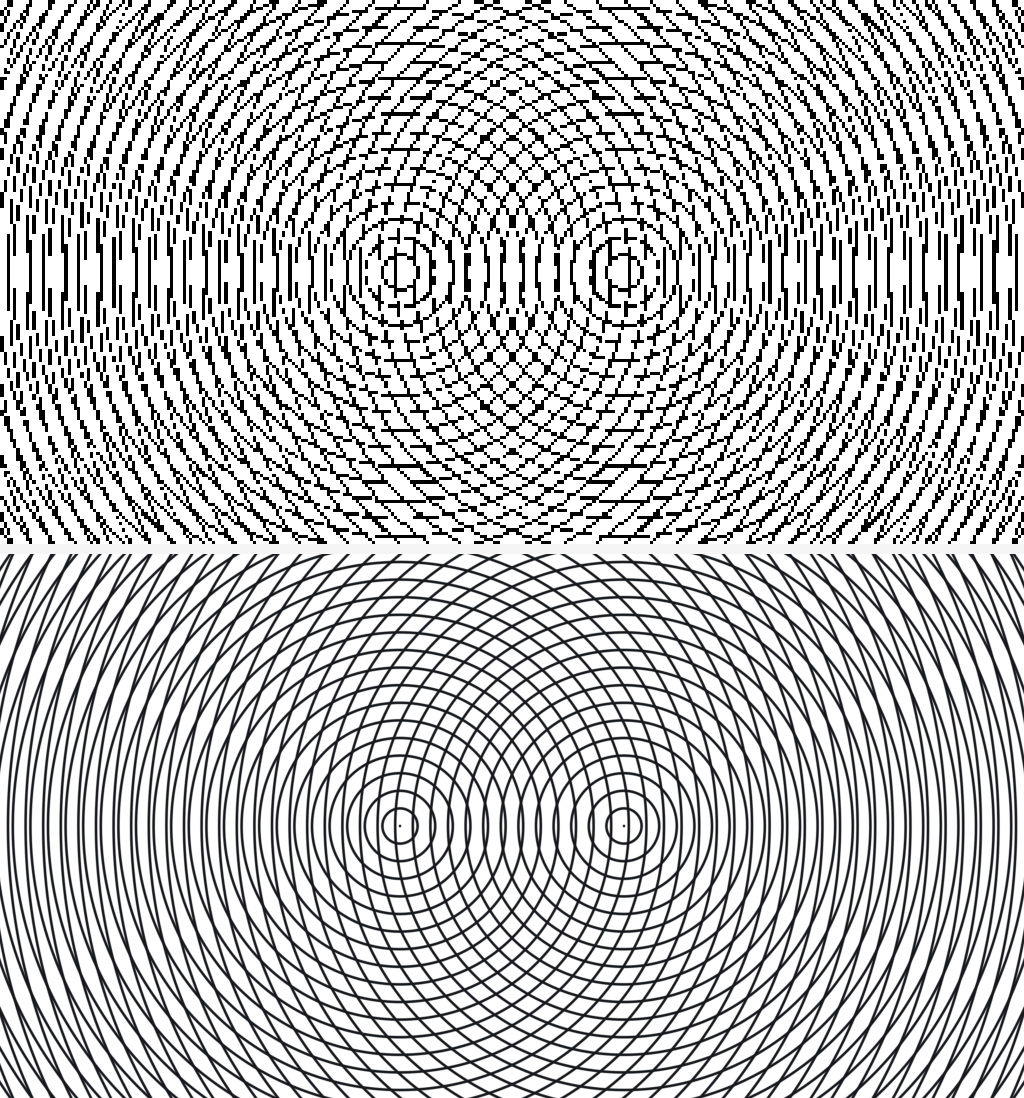
\includegraphics[width=\linewidth]{figures/two-traditions.png}
  \Description{Two square black-on-white panels stacked. Both show two sets of
  concentric rings about different centers, crossing to form a lens-shaped fringe
  pattern. In the upper panel the rings are broken into ragged dashes, the outer rings
  have faded to gray mush, and a coarse blotchy pattern sits over everything. In the
  lower panel every ring is a continuous crisp line right into the corners and the
  only large-scale pattern is the fringe system itself.}
  \caption{\figlead{Raster versus field, same two families.} \emph{Above:} the
  standard synthesis pipeline reused at a scale it was not rasterized for. Each
  layer is rasterized to a bilevel plate, the plates are multiplied, and the
  product is displayed at a different scale, which is what photographing,
  scanning or zooming a printed pair amounts to. (Printed at press resolution and
  viewed in place, the plates never resample; every \emph{screen} reuse of them
  does, and the screen is where an interactive tool lives.) The strokes break into dashes, the
  outer rings dissolve, and a coarse secondary pattern appears that is a property of
  the sampling grid rather than of either family. \emph{Below:} the same two
  families as fields. Two distance queries per pixel, composited, at the display
  resolution. There is no intermediate raster, so the sampling grid contributes
  no pattern of its own, and the crossings stay crisp all the way to the corners.}
  \label{fig:traditions}
\end{figure}

A layer, stripped of its raster, is a countable family of curves
$\{\gamma_n\}$: the $n$th line, the $n$th ring, the $n$th turn of a spiral.
We represent a pattern as a pair $(\cnt,F)$. The \emph{counting map}
$\cnt\colon M\to\T^K$ names the members, fractionally, one coordinate per
family; the \emph{ink} $F$ paints the torus, and the image is $F\circ\cnt$.
The distance field is the leading term of $F$. The index field of a
scalar family is one coordinate of $\cnt$. Superposition is the joint
map. Our central observation is that the interference lives entirely in
$\cnt$: \emph{the visible beat is an integer character $k\cdot\cnt$, and
the fringes are its unit level sets}. Section~\ref{sec:fringe} makes this
precise: the locally averaged ink is a function of $D=\idx_1-\idx_2$
alone, a saturating tent rather than a sinusoid, exact under stated local
hypotheses and first-order accurate beyond them. The same section verifies
the law against $\fringeSamples$ measurements over $\fringeScenes$ pairs of
families, to a mean coverage error of $\fringeMeanErr$.
The locus and the profile shape have classical
ancestors~\cite{Oster1964, Patorski1976Profile, Amidror1994TConv}; what the
counting-map form adds is a per-pixel statement about the actual compositing
operator, with a computable validity criterion: the heterodyne ratio $\het$, a
\emph{field} that can be drawn, telling an author where in the frame a fringe
will form before they commit to parameters. A family's index convention is
arbitrary, so $D$ is one representative of a lattice of integer combinations
$k_1\idx_1+k_2\idx_2$, and the visible moir\'e is whichever combination beats
slowest against the contrast its order costs (\S\ref{sec:visibility}).
Which combination that is turns out to be a best-approximation question
with a classical answer: the visible-beat hierarchy of two pitches is the
continued fraction of their ratio, and in two dimensions the winner is found
exactly, at any order, by per-pixel lattice reduction (\S\ref{sec:selection}).

The catalog sits on an integrability ladder (Section~\ref{sec:object}).
Nine of the thirteen families we ship are exact: parallel lines precomposed
with a field, one line of algebra each. The radial pencil is a defect of
that line family. The families that make the richest interference are the
fold rung. What op artists actually reach for are families whose members
are not concentric: each ring displaced a little further than the last, or
turned a little further, so the family shears, spirals, and finally
unwinds into a pencil of near-parallel curves; Riley's \emph{Blaze}, a nest
of zigzag rings each turned against the last, is exactly such a
family~\cite{Oster1965Optical}. We call these \emph{walking families}
(Section~\ref{sec:walking}): member $n$ is the shape of radius
$ns+\varphi$, displaced by $n\delta$ and turned by $n\theta$. Two extra
parameters, and the closed form is gone. Search is the price of
non-integrability. The obvious search, guess the index from the radius and
check a fixed number of neighbors, fails coherently: the pixels whose true
nearest member falls outside the guessed neighborhood form arcs, not
speckle, so whole sides of whole rings disappear, and the budget is paid at
every pixel whether or not it was needed. For a long time we believed these
broken segments were a rasterization bug; they are an inversion bug.

Section~\ref{sec:inverse} replaces the guess with a certificate. Every radial
metric in this setting (circle, square, triangle, regular $N$-gon) is a
\emph{support function}, and support functions supply exactly the constants the
problem needs: a Lipschitz modulus that lets indices be skipped unevaluated, in
the spirit of sphere tracing~\cite{Hart1996Sphere}; an exact anisotropy floor;
and a subadditive drift rate $\rad(-\delta)$ that is strictly tighter than
$\lVert\delta\rVert$, where using the loose constant declares whole bands of
ordinary settings unsolvable. Together they give a closed interval of integers
that provably contains every member passing within a stroke width of the pixel
(an interval that, unexpectedly, does not involve the rotation $\theta$ at
all) and, when $\theta=0$, a closed form for translated polygons of any side
count, including a marginal case in which the residual is eventually constant
and no enumeration of any finite length can succeed. Measured on the GPU the
certified solver is $\gpuSpeedLo$--$\gpuSpeedHi\times$ faster than the fixed
enumeration it replaces across rotated settings, at equal or better fidelity,
and faster than an exhaustive scan given the same termination bound. Where the
interval genuinely explodes, on the tangent-pencil locus where unboundedly
many members really do crowd a point, Section~\ref{sec:limits} shows the
choice that matters is not how much to subsample but how: anchored to the
family, the error reads as a thinner pattern; anchored to the pixel, as a
shattered one, at identical cost.

\subsection{Contributions}

\begin{itemize}
  \item A counting-map formulation of moir\'e: a pattern is
  $(\cnt,F)$, superposition is a joint torus, and the catalog is an
  integrability ladder of rank times exact / defect / fold
  (Section~\ref{sec:object}). The pattern has no raster at any stage.

  \item The fringe law: locally averaged ink is a saturating tent in the index
  difference, so fringes are its unit level sets. The law is exact under stated
  local hypotheses, per-pixel, with no periodicity assumption, and with a computable
  validity criterion, the heterodyne ratio, drawable as a map
  (Sections~\ref{sec:fringe}--\ref{sec:visibility}).

  \item The selection principle: which beat is visible is best approximation,
  answered by continued fractions in one dimension and by per-pixel
  Lagrange--Gauss reduction of the gradient lattice in two, under an amplitude
  weight that makes ``slowest visible beat'' well posed. The reduction
  replaces an order cap that missed $\selCapMissPct\%$ of visible fringes in
  random carrier pairs, and its winner drives the criterion, the envelope's
  sweep schedule, and the contour overlay (\S\ref{sec:selection}).

  \item Folds and their inversion: walking families, whose index has no
  closed form, and a provably sufficient index interval from the support
  function of the generating shape, a Lipschitz skip rule, and an exact
  closed form for translated polygons of any side count including the
  marginal drift (Section~\ref{sec:inverse}, Appendix~\ref{app:proofs}).

  \item \Moire{}, an interactive tool: thirteen families, twelve concurrent
  layers compiled once, zoom-stable strokes, GPU type morphing, and no
  rasterization step (Section~\ref{sec:system}). Its \emph{envelope} view draws
  the averaged ink directly, which requires averaging over index rather than
  over space; done properly it costs one solve and a few instructions per tap
  rather than one solve per tap (Section~\ref{sec:envelope}).

  \item Moir\'e as a contouring primitive, the corollary of the affine space
  of exact patterns (\S\ref{sec:object}): encoding a scalar field in an
  index difference renders its contours without ever computing a contour.
  The fringes localize to a mean of $\contourWorstErr$\,px of the true
  level sets on the hardest field we tested
  (Section~\ref{sec:beyond}). A circle-valued field mints topological
  defects: fringes that end, with the signed count of endings equal to the
  enclosed winding times the gain, exactly (Section~\ref{sec:defects}).

  \item An expression language for those fields, with the gradient the eikonal
  divide needs obtained by forward-mode differentiation rather than by hand, and
  compiled to straight-line shader code rather than interpreted per pixel. The
  compilation is what makes an arbitrary user-written field affordable:
  $\fieldGainLo$--$\fieldGainHi\times$ cheaper than the interpreter it replaced
  (Section~\ref{sec:exprs}).
\end{itemize}

\section{Related work}
\label{sec:related}

\paragraph{Spectral theory.}
The standard account of moir\'e is spectral. Superposing two transparencies
multiplies their intensities, so their spectra convolve, and the convolution
produces sum and difference components that were in neither layer. When two
carriers are close, the $(1,-1)$ difference component falls below the eye's cutoff
and appears as a large, slow pattern. Amidror's monograph is the complete
treatment~\cite{Amidror2009Theory}, developed with Hersch across a sequence of
papers that moves from analysis of screen interactions~\cite{Amidror1994Spectral},
to phase shifts~\cite{Amidror1996Fourier}, to synthesis under geometric
transformation~\cite{Amidror1998Fourier}, and finally to aperiodic
layers~\cite{Amidror2003Moire, AmidrorII}, whose random-dot extreme is the Glass
pattern~\cite{Glass1969Moire}. The account is still growing: Feng extends it to
\emph{objective} structures --- ring, helical and lattice patterns whose members
are related by progressive symmetry transformations --- through an augmented
Fourier approach~\cite{Feng2025Objective}. Those structures are the closest
formal relatives of our walking families (\S\ref{sec:walking}), reached from the
frequency side; we reach them per pixel, with a certificate, because a renderer
has to. That is the general shape of our debt to this theory: it tells you
\emph{that} a fringe exists and where its frequency lies, but it is a statement
about spectra of images, not a renderer.

\paragraph{The indicial equation.}
Running alongside the spectral account is an older and more elementary one. Label
the members of each layer, ask where a member of one crosses a member of the other
in a fixed relation, and solve: Oster, Wasserman and Zwerling derive the fringe
curves of the standard configurations this way~\cite{Oster1964}, Amidror gives
it as the geometric approach, complementary to the spectral one --- curved
gratings read as indexed line families (Vol.~I, \S11.2
of~\cite{Amidror2009Theory}) --- and the metrology literature develops it at
book length~\cite{Bryngdahl1974Moire, Patorski1993Handbook}. This is the direct ancestor of our
Section~\ref{sec:fringe}, and our index field is its label made continuous and
evaluated per pixel. We claim no credit for the locus. What the indicial method
does not supply is the quantity a renderer needs --- the coverage \emph{between} the
fringes --- nor any statement of when the construction is meaningful; our
Theorem~\ref{thm:fringe} supplies the first as a closed-form profile of the actual
compositing operator and \S\ref{sec:visibility} the second as a field that can be
drawn. Both are per-pixel, exact rather than asymptotic, and indifferent to whether
anything is periodic.

\paragraph{Constructive synthesis.}
Band moir\'e~\cite{Hersch2004Band} is the landmark generation method in graphics:
a base layer of image bands, replicated and compressed along one axis, sampled by a
revealing line grating, with a derived linear map from band space to moir\'e space
that predicts the revealed image's orientation, scale and velocity. Applying
nonlinear coordinate transforms to both layers yields curved layers whose
superposition is still a clean periodic moir\'e. Level-line
moir\'e~\cite{Chosson2014Beating} changes the encoding: a bilevel target becomes an
elevation profile, embedded as small local displacements of the base grating, and
the superposition reveals the profile's \emph{level lines}, which traverse the
shape as the layers slide. Walger and Hersch multiplex up to seven such images in
one base~\cite{Walger2015Hiding}. Target-driven phase
modulation~\cite{Tsai2013Target} is the strongest inverse formulation: given a
grayscale target, solve for two curvilinear gratings whose dominant difference
component reproduces it, with a smoothness term distributing information between
the layers and an appearance phase to disguise them. Lebanon and
Bruckstein~\cite{Lebanon2001Variational} give the variational counterpart.

These methods and ours are close in spirit and disjoint in mechanism. They solve
an inverse problem to \emph{produce} two layers; we make the forward problem cheap
enough that a person can solve the inverse problem by hand, in real time, at any
zoom. The level-line formulation is the closest relative, and the relationship is
clean: their construction embeds a designed elevation profile in a grating's phase
so that its contours appear as fringes, and our Section~\ref{sec:beyond} shows
that in the field model this is not a construction at all but an immediate
consequence of the fringe law, available for any field, on screen, with no printing
step. We regard that as evidence the representation is the right one, not as a
claim to have invented level-line moir\'e.

\paragraph{Halftoning.}
Halftoning is where moir\'e is classically a hazard and occasionally a tool.
Rotated dispersed dither disperses the spectral impulses of a Bayer array so that
colour separations do not beat~\cite{Ostromoukhov1994Rotated, Ulichney1987};
multi-colour dithering extends the control to non-standard
inks~\cite{Ostromoukhov1999MultiColor}. Artistic
screening~\cite{Ostromoukhov1995Artistic} turns the halftone dot into an
artist-supplied contour that grows with intensity and can be pushed through a
conformal map, which makes the screen itself the designed object --- the direct
conceptual ancestor of band moir\'e, and a useful reminder that the expressive
material here is the \emph{carrier}, not the picture.

\paragraph{Physical realisation and sensing.}
Moir\'e magnifiers pair a micro-image array with a slightly mismatched lens
array~\cite{Hutley1994Moire}. EPFL's later work replaces printed revealers with
cylindrical microlenses~\cite{Walger2019Moire, Walger2020LevelLine} and Saberpour
et al.\ carry designed moir\'e onto curved fabricated
surfaces~\cite{Saberpour2020Fabrication}. Refractive
steganography~\cite{Papas2012Magic} and metallic-substrate
hiding~\cite{Pjanic2015Color} pursue the same hidden-image goal by other optics.
Running the amplification backwards turns a moir\'e into a precise passive
encoder: MoiréBoard for camera pose~\cite{Xiao2021MoireBoard}, MoiréTag for
angle~\cite{Qiu2023MoireTag}, MoiréWidgets for tangible
controls~\cite{CamposZamora2024MoireWidgets}. These works establish that the phase
of a moir\'e is a quantity worth measuring to high precision, which is indirectly
an argument for having it available in closed form.

\paragraph{Interactive authoring.}
FabObscura~\cite{Sethapakdi2025FabObscura} is the nearest system-shaped relative:
it parameterises barrier-grid occlusion patterns as functions, and couples a
pattern editor to a live canvas and a fabrication export. Barrier-grid animation
is a parallax technique rather than interference, so the mechanism differs, but its
design stance --- find the right parameterisation, then expose it directly rather
than making the user reason about pixels --- is the one we tried to adopt. Outside
archival venues, procedural moir\'e is a staple of shader practice, going back to
Glassner's tutorial treatment~\cite{Glassner1997Inside} and Sen's product-delay
constructions~\cite{Sen1998Product, Sen2000Moire}, in the wider tradition of
evaluating a pattern per point rather than storing it~\cite{Ebert2003Texturing}.
The shader-sandbox idiom is
essentially universal and essentially always the same: evaluate two periodic
functions and combine them, typically as \texttt{abs(p1 - p2)}. That is a
\emph{value} composite rather than a distance composite, and
Section~\ref{sec:zoom} shows what it costs --- there is no stroke width to
stabilise, so the pattern is a different pattern at every zoom level, and the
displayed moir\'e is partly the sampler's own.

\paragraph{Moir\'e in visualization.}
Direct use of interference to encode data is rare. MoireGraphs is the notable
appearance of the word in the visualization literature, and it names a
resemblance: a radial focus+context layout whose concentric rings of visual nodes
\emph{look} like a circular moir\'e~\cite{JankunKelly2003Moire}. The place where
fringes genuinely carry data is experimental mechanics and optical metrology.
Moir\'e interferometry reads in-plane displacement: fringes are contour maps of
displacement, with fringe order $N_x=fU$ for reference grating frequency $f$,
and strains follow by differencing fringe orders~\cite{Post2008Moire,
Post1994High}. Moir\'e topography reads surface height the same way --- its
fringes literally are elevation contours~\cite{Takasaki1970Moire,
Meadows1970Contours} --- and Takeda's Fourier-transform method turned fringe
images back into phase maps numerically~\cite{Takeda1982Fourier}. These are
measurement techniques, and their governing relation is exactly our fringe law
read in the other direction. Section~\ref{sec:beyond} takes it as a design
primitive instead: the encoded field is arbitrary, on screen, and live.

\paragraph{Distance fields and certified search.}
The machinery we borrow from is the distance-field tradition: guaranteed
intersection from a Lipschitz constant~\cite{Kalra1989}, sphere tracing, which uses
such a bound to skip space it can prove is empty~\cite{Hart1996Sphere}, and its
sharpening by \emph{local} Lipschitz bounds along a segment~\cite{Galin2020};
adaptively sampled distance fields as a shape
representation~\cite{Frisken2000Adaptively}; and the now-standard practice of
shading vector art from a distance rather than a coverage
mask~\cite{Green2007Improved, Quilez, Quilez2019Distance}. Our index window
(Section~\ref{sec:window}) is a sphere-tracing argument moved from space into
\emph{index} space, and our skip rule is segment tracing along the index axis:
where a ray marcher steps by the distance it can prove is empty, we step by the
number of \emph{rings} we can prove cannot be nearest. The alternative discipline,
enumerating every cell a ray meets~\cite{Amanatides1987}, is what the fixed sweep
we replace amounts to. The closest methodological neighbours are the range-analysis
renderers, which bound a function over a spatial cell and subdivide until the
bound decides~\cite{Knoll2009, Keeter2020, Sharp2022}. Section~\ref{sec:discussion}
argues that our domain being $\Z$ rather than $\R^2$ is what upgrades their
tolerance into a certificate. Seen from optimization, the certified scan is a Piyavskii--Shubert
search~\cite{Piyavskii1972, Shubert1972} run over $\Z$ instead of an interval of
$\R$: the same Lipschitz envelopes, with the stopping tolerance replaced by
integer exhaustion. The support-function facts we need are standard
convex geometry~\cite{Rockafellar1970Convex, Schneider2014Convex}, and the same
object is what collision detection queries when it walks a Minkowski
difference~\cite{GJK1988, Ericson2004} --- though there it prices one pair of
bodies, where here the certificate ranges over an indexed family of them; our
contribution is noticing which four of its properties this problem is asking
for.

\paragraph{Prefiltering a pattern.}
Where a procedural pattern is too fine to sample, the correct answer is to
integrate it rather than to point-sample harder, a line that runs from the
frequency analysis of aliasing~\cite{Crow1977, Mitchell1990} through the
analytically prefiltered procedural textures surveyed by Lagae et
al.~\cite{Lagae2010} to normal-distribution methods for glinty
surfaces~\cite{Yan2014, Yan2016}. Two things connect that work to ours. Our
saturated regime (\S\ref{sec:limits}) is exactly a place where a correct analytic
mean would replace a fallback we know to be approximate, and we do not have one for
a walking family. And the glint problem has our structure --- ``which member of a
dense indexed family lies within this footprint'' --- solved with a
budget~\cite{Yan2016} where an index interval might certify.

\section{Moir\'e as a field}
\label{sec:field}

\subsection{A layer is two scalar fields}

\begin{definition}[Family]
A \emph{family} is a countable collection of curves $\{\gamma_n\}_{n\in\Z}$ in
$\R^2$, together with an index convention that names them.
\end{definition}

We never represent $\{\gamma_n\}$ as geometry. A layer is represented by two
functions of a continuous position $p\in\R^2$:
\begin{align}
  \idx(p) &\in \R && \text{the \emph{index field}: } \gamma_n=\idx^{-1}(n),\\
  d(p) &= \min_{n} \mathrm{dist}(p,\gamma_n) && \text{the \emph{distance field}.}
\end{align}
The index field is fractional --- $\idx(p)=7.3$ means $p$ lies three tenths of the
way from member $7$ to member $8$. The distance field is Euclidean and unsigned.

Most families in practice are the level sets of a single scalar \emph{phase}
function. It is convenient to keep the phase in world units, so that member $n$ is
the level set $\{\ph = ns + \varphi\}$ with $s$ the spacing and $\varphi$ an
offset. Then
\begin{equation}
  \idx(p) = \frac{\ph(p)-\varphi}{s},
  \qquad
  d(p) \;\simeq\; \frac{\mathrm{pd}\!\left(\ph(p)-\varphi,\; s\right)}{\lVert\nabla\ph(p)\rVert},
  \label{eq:eikonal}
\end{equation}
where $\mathrm{pd}(v,s)=\min_{k\in\Z}|v-ks|$ is the distance from $v$ to the
lattice $s\Z$. Both are one line of shader code.

\subsection{The gradient is not optional}
\label{sec:eikonal}

\begin{figure}[t]
  \centering
  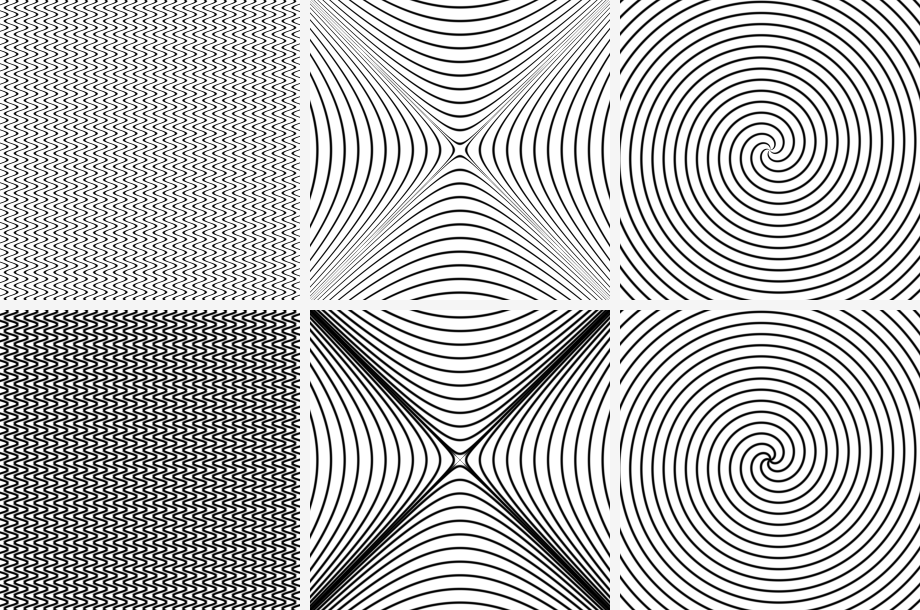
\includegraphics[width=\linewidth]{figures/gradient-compare.png}
  \panelrow{0.32609}{0.01087}{wave, hyperbola, spiral}
  \Description{A two-by-three grid of black-on-white panels: a wave family, a
  hyperbola family and a spiral family, drawn twice. In the top row the strokes fade
  to nothing towards the edges where the curves crowd together; in the bottom row
  those same regions are solid black.}
  \caption{\figlead{A phase residual is not a distance.} Top: what our shader drew
  for the wave, hyperbola and spiral families --- the phase residual, undivided.
  Strokes thin by exactly the factor the family is steep by, so the pattern fades
  where it should saturate and the hyperbola's asymptotes disappear. Bottom: the
  same settings with Eq.~\ref{eq:eikonal}. The parabola family always divided; these
  three did not, and the failure is worst exactly where the family is densest.}
  \label{fig:gradient}
\end{figure}

The division by $\lVert\nabla\ph\rVert$ in Eq.~\ref{eq:eikonal} converts a phase
residual into a length. It is easy to omit, and we omitted it. Our shader applied
it for the parabola family and not for the wave, hyperbola or spiral, with two
consequences.

The first is cosmetic but severe. Where $\lVert\nabla\ph\rVert=g>1$, the reported
distance is $g$ times too large, so the stroke is $g$ times too thin. Sweeping each
family over its own slider range on a $1400\times880$ frame
(Appendix~\ref{app:atlas}, Table~\ref{tab:gradient}) we measure $g$ up to
$\gradWorstWave$ for the wave and $\gradWorstHyp$ for the hyperbola, with more than
half the frame off by over $10\%$ in both cases. Visually the family pales out
exactly where it steepens and crowds --- the opposite of what the geometry does
(Figure~\ref{fig:gradient}).

The second is a correctness bug. Our stroke half-width is
$\mathrm{halfT}=\max(t/2,\,1.15\,\mathrm{px})$, and the floor exists so that a
hairline stays a hairline instead of breaking into speckle when zoomed out
(Section~\ref{sec:zoom}). That floor is a statement about \emph{screen} distance.
Compared against an undivided phase residual it is a statement about phase, and it
guarantees nothing wherever $g\neq1$. The families that most need the floor --- the
steep ones --- are precisely the ones that were not getting it.

We adopt Eq.~\ref{eq:eikonal} everywhere. One honest cost: a wave at high amplitude
and frequency now saturates to solid ink, because at those settings its members
genuinely are closer together than a stroke width. That is the correct answer, and
the previous behaviour was hiding it.

Eq.~\ref{eq:eikonal} is an eikonal approximation and it is exact only where the
family is locally a foliation with steady gradient. The one family in our
catalogue that violates this is the hyperbola, whose level sets cross on its
asymptote cross; we return to it in Section~\ref{sec:limits}.

\subsection{Compositing}

Layers composite as ink over paper. With stroke half-width $h_i$ and antialias
band $a$, layer $i$ contributes coverage
\begin{equation}
  \alpha_i(p) = \Big(1-\mathrm{smoothstep}(h_i-a,\;h_i+a,\;d_i(p))\Big)\,o_i,
  \label{eq:alpha}
\end{equation}
and the frame is the running \texttt{mix} of background with each layer's colour
at that alpha. For two black layers on white this is the union
$\alpha_1+\alpha_2-\alpha_1\alpha_2$. There is no separate composite pass, no
intermediate texture, and no place in the pipeline where a layer exists as pixels.

Three properties follow immediately and are the practical reason to do it this way.

\emph{No resolution.} $\idx$ and $d$ are defined at every real position, so
changing zoom changes only where they are sampled. A moir\'e authored at one scale
is the same moir\'e at another (Section~\ref{sec:zoom}).

\emph{Bounded frequency by construction.} The stroke floor
$h\ge1.15\,\mathrm{px}$ means the ink field's transition band is never narrower
than a pixel, so the composite is band-limited without any filtering step. This is
the thing the suppression literature achieves with prefiltering and the synthesis
literature cannot achieve at all: we get to keep the designed difference component
and lose the undesigned ones, because the undesigned ones are never created.

\emph{Editability.} Every parameter enters $\idx$ and $d$ analytically. Moving a
slider does not invalidate a cached raster, because there is none.

\subsection{The fringe law}
\label{sec:fringe}

Now the observation the rest of the paper rests on. Superpose two layers. Where
does the visible pattern come from?

Fix a point $p$ and let $D=\idx_1-\idx_2$ be the difference of index fields. Write
$w_i$ for layer $i$'s stroke half-width measured \emph{in index units},
$w_i=h_i\lVert\nabla\idx_i\rVert$, and $b_i=a\lVert\nabla\idx_i\rVert$ for its
band. Define the index-space stroke profile
$A_i(u)=1-\mathrm{smoothstep}(w_i-b_i,\,w_i+b_i,\,\mathrm{pd}(u,1))$.

\begin{theorem}[Fringe law]
\label{thm:fringe}
Let $u$ be the direction of the mean index gradient
$g=\tfrac12(\nabla\idx_1+\nabla\idx_2)$, let $T=1/\lVert g\rVert$ be the carrier
period, and let $S=p+[-T/2,T/2]\,u$. Suppose that on $S$ both families are local
foliations and that $D$ is constant. Then the mean ink over $S$ is
\begin{equation}
  \label{eq:phi}
  \begin{gathered}
    \bar\alpha(p) \;=\; \Phi\big(D(p)\big), \qquad\text{where}\\
    \Phi(g) \;=\; \int_0^1 \Big[A_1(v)+A_2(v-g)-A_1(v)A_2(v-g)\Big]\,\mathrm{d}v,
  \end{gathered}
\end{equation}
which depends on $p$ only through $D(p)$. If instead $D$ is merely affine on $S$,
the same expression holds up to an error $O(\het)$ in the ratio \eqref{eq:ratio}
below. In the hard-edged limit $b_i\to0$,
\begin{equation}
  \Phi(g) = 2w_1+2w_2-\max\!\big(0,\;w_1+w_2-\mathrm{pd}(g,1)\big):
  \label{eq:tent}
\end{equation}
a tent in $D$, rising from $2\max(w_1,w_2)$ at $D\in\Z$ to a plateau of
$2w_1+2w_2$ once the strokes clear each other.
\end{theorem}

The proof is a change of variables and is given in Appendix~\ref{app:fringe}; the
content is entirely in the statement. It is worth being exact about the two
hypotheses, because they are not interchangeable. ``Both families are local
foliations on $S$'' is what lets us reparameterise the segment by index instead of
by arclength. ``$D$ is constant on $S$'' is what makes the answer a function of
$D(p)$ alone, and it is the strong one: exact constancy means the two carriers
agree exactly in pitch and direction, so the interesting cases only satisfy it
approximately. The appendix carries the affine case through and shows the
correction is first order in $\het$, which is the same small parameter
\S\ref{sec:visibility} uses to decide whether a fringe exists at all. So the
theorem is exact in the limit that a fringe becomes infinitely broad, and
degrades in the parameter that measures how far from that limit we are --- which is
why the verification below both restricts to $\het\le1/4$ and reports the residual
rather than claiming zero. Three further things are worth saying.

\paragraph{The locus is classical; the profile is not.}
$\Phi$ is periodic with period $1$ and extremal at $D\in\Z$ and
$D\in\Z+\tfrac12$. So the light fringes are exactly $\{D\in\Z\}$ --- where the two
families' members locally coincide and their strokes overlap, wasting ink --- and
the dark fringes are exactly $\{D\in\Z+\tfrac12\}$, where the members interleave
and the ink is maximally spread. \textbf{The moir\'e is the contour plot of
$\idx_1-\idx_2$ at unit interval.} Nothing else about either family survives the
average.

That locus is not ours and we want to be exact about whose it is. Writing the two
families as $\idx_1=m$, $\idx_2=n$ and asking where their members cross in a fixed
relation $m-n=k$ is the \emph{indicial equation}, which is how Oster, Wasserman and
Zwerling read moir\'e in 1964~\cite{Oster1964} and how Amidror presents the
geometric approach~\cite{Amidror2009Theory}; the same relation, read backwards, is
the fringe-order law of moir\'e
interferometry~\cite{Post2008Moire}. If the reader's summary of
Theorem~\ref{thm:fringe} is ``the fringes are the unit level sets of the index
difference'', they have learned nothing after 1964, and should stop there.

What the theorem adds is everything to the left of the locus. The classical
argument identifies a set of curves; it does not say what \emph{value} the frame
takes between them, and a renderer has to produce that value at every pixel. $\Phi$
does: it is the mean coverage of the actual compositing operator
(Eq.~\ref{eq:alpha}), so it carries the stroke widths, the saturation, and the
antialias band, and it holds where nothing is periodic, where the two carriers are
different families, and per-pixel rather than in the asymptotic limit of a
grating pair. It comes with $\het$ (\S\ref{sec:visibility}), which says where it
may be trusted --- the classical accounts assume the near-matched regime rather
than measuring it. And because it is a formula for averaged ink rather than a set
of curves, it can be \emph{drawn} (\S\ref{sec:envelope}) and it can be
\emph{inverted} (\S\ref{sec:beyond}). Those are the parts we lean on.

\paragraph{It is a tent, not a sinusoid, and it saturates.}
Grating models built on the first Fourier component predict a sinusoidal fringe
profile. Eq.~\ref{eq:tent} says the profile is piecewise linear with a flat top,
and the flat top is reached as soon as $\mathrm{pd}(D,1)>w_1+w_2$. This is why
field-composited moir\'e looks crisper than the same pattern built spectrally: most
of the fringe is at full contrast, and the transition occupies only a
$(w_1{+}w_2)$-wide sliver of each period. It also explains a design behaviour we
had noticed but not understood --- past a certain stroke thickness, thickening the
strokes stops changing the fringe and only darkens the whole frame.

\paragraph{No periodicity is required.}
$\idx_1$ and $\idx_2$ are arbitrary. The theorem's hypotheses are local
(affineness of $D$ over one carrier period, and the eikonal condition) and say
nothing about global structure. A spiral is admissible. Two hyperbola families are
admissible. A pencil of rings each rotated by $n\theta$, which is not a geometric
transform of any periodic layer, is admissible.

\subsection{The envelope view}
\label{sec:envelope}

$\bar\alpha$ is a quantity, so it can be drawn, and drawing it gives the author
the fringe system with the carrier removed. The obvious way to get such a picture
is to blur the render, and it is the wrong way: a blur is a kernel in pixels, so
it changes under zoom, it softens every real edge along with the carrier, and its
width has to be retuned whenever the pitch changes.

Look again at the hypothesis of Theorem~\ref{thm:fringe}. Over the averaging
segment every family's index advances by the \emph{same} amount --- that is what
$D$ constant means --- so the entire stack is a one-parameter object. Advance every
layer's index together by $u$ and average over $u\in[0,1)$:
\begin{equation}
  \bar\alpha(p) \;=\; \int_0^1 \alpha\big(p;\; \idx_i \mapsto \idx_i + u\big)\,\mathrm{d}u.
  \label{eq:meanink}
\end{equation}
This is an average over \emph{index}, not over space. No sample is taken off
centre, so nothing is blurred; the result is the theorem's own $\bar\alpha$ at the
full resolution of the frame, and it is identical at every zoom. Since the
integrand is periodic in $u$ with period exactly $1$, a uniform grid of $M$ nodes
is exact but for harmonics above $M$; the integrand is a composite of trapezoids,
so $M=\envTaps$ leaves an error far below one colour step. Every ``averaged ink''
panel in this paper is \eqref{eq:meanink} at $M=\envTaps$, and it is a toggle in
the Studio, not a post-process.

Written that way, \eqref{eq:meanink} is an integral over the diagonal of the
\emph{index torus} $[0,1)^K$ --- one circle per family --- and the choice of the
diagonal is exactly Theorem~\ref{thm:fringe}'s hypothesis rather than a
convenience. It is worth saying what the honest alternative is, because we
implemented it first. Sweeping a rigid translation of the whole stack is
geometrically exact where advancing an index is bookkeeping, and it is unusable:
the taps then sample a two-dimensional disc for strokes that cover a few percent
of it, so a handful of taps carry the answer and the rest carry noise. Sixty-four
of them left the carrier standing and the fringes mottled. The diagonal's fiction
is what makes it exact.

\paragraph{One solve, many taps.}
The cost, done naively, is $M$ full evaluations of every layer --- and for a
walking family one evaluation is the search of \S\ref{sec:inverse}, so $\envTaps$
of them per pixel is not a view, it is a stall. It was: our first envelope ran at
five frames a second on the tool's own opening preset.

It need not, and the reason is that advancing an index by less than one does not
change \emph{which} members are nearby. So the solver is asked once per pixel for
a \emph{phase sample}
\begin{equation}
  \Pi(p) \;=\; \big(\,\rho,\; \rho^{\uparrow},\; \rho^{\downarrow},\; \ell\,\big),
  \label{eq:phasesample}
\end{equation}
the signed distances to the nearest member and to the two flanking it, together
with a floor $\ell$ that does not participate. A tap at $u$ then reads
\begin{equation}
  d(p;u) \;=\; \max\Big(\min_{k\in\{\rho,\rho^{\uparrow},\rho^{\downarrow}\}} \lvert k - u\,g \rvert,\; \ell\Big),
  \label{eq:slide}
\end{equation}
where $g=\lvert\rho^{\uparrow}-\rho\rvert$ is the \emph{local} member gap. Because
the sweep is centred on $u=0$, the triple brackets every phase it visits, so
\eqref{eq:slide} is not an approximation of the re-solved distance --- it is that
distance, in nine instructions. The search runs once per pixel and the sweep is
arithmetic. Median frame times in the envelope view went from hundreds of
milliseconds to inside the frame.

Two things fall out of writing the sample this way. The gap $g$ is local, so a
tap covers exactly one period of \emph{this} family at \emph{this} point, whatever
the pitch does across the frame --- which is what the radial pencil needs, since
its member gap $2r\sin(\pi/2N)$ grows with radius. And $\ell$ is where the
non-sliding parts of a family live: the guard returned by a saturated solve, the
hole at the centre of a pencil, the missing inner neighbour of the innermost
hyperbola. Those are the places where there is genuinely nothing to slide onto,
and separating them from the residual is what keeps the average from inventing
ink there.

\paragraph{Every family has a currency.}
Equation~\ref{eq:meanink} advances an index, and each family spends that in its
own coin. The level-set families of \S\ref{sec:catalog} shift a phase. The radial
pencil turns: advancing its index by $u$ rotates the fan by $u\pi/N$, which is
how a family whose index is an angle joins an average built for scalars. A lattice
indexes its members by a \emph{pair} of integers, so it translates along its two
generators --- and here the diagonal is exactly wrong. Stepping both generators in
lockstep keeps their two indices correlated, and a lattice then beats against
itself: a fine diagonal hatch at the carrier's own scale that no amount of
contrast can be read through. So we take the $i$th tap along the first generator
to $u_i$ and along the second to $\{i\varphi\}$, $\varphi$ the golden ratio ---
the Fibonacci lattice, a rank-1 rule on the
two-torus~\cite{Sloan1994Lattice, Keller2013Quasi}. It decorrelates a lattice from
itself while leaving it in step with every other layer's matching generator, which
is where the fringes an author wants actually are.

\paragraph{A pivot, not a gain.}
The view exposes a contrast, because a fringe field is a small excursion about the
stack's mean coverage and the interesting part is the excursion. Expanding about
$0$ would ride the mean up and down as the fringes move, so the expansion is about
the coverage the stack would average over its own periods: $2h/s$ per family,
composited. Counting a lattice's families is not optional. A hex lattice draws
three, and calling its coverage that of one puts the pivot far brighter than the
picture it is expanding about, which at any real contrast drives the whole frame
black --- which is precisely how we found the bug.

One caveat remains, and it is structural rather than a matter of implementation.
The average is over the diagonal, so where Theorem~\ref{thm:fringe}'s hypothesis
fails --- where $\het$ is large --- the view still shows $\Phi(D)$ faithfully, but
$\Phi(D)$ is no longer what the eye will average. The honest reading of the two
together is the ratio map beside the envelope.

\subsection{When is there a fringe at all?}
\label{sec:visibility}

Theorem~\ref{thm:fringe} needs $D$ to be nearly constant over one carrier period.
Both requirements are about the same ratio. Define the \emph{heterodyne ratio}
\begin{equation}
  \het(p) = \frac{\lVert\nabla D(p)\rVert}{\lVert g(p)\rVert}
  = \frac{\lVert\nabla\idx_1-\nabla\idx_2\rVert}
         {\big\lVert\tfrac12(\nabla\idx_1+\nabla\idx_2)\big\rVert}.
  \label{eq:ratio}
\end{equation}
$D$ changes by $\het$ across one carrier period, so $\het\ll1$ is exactly the
condition that a fringe be large compared with the carrier. It is the field-space
form of the classical requirement that the two frequencies be close --- and it is a
\emph{field}, so it varies over the frame, and it can be drawn
(Figure~\ref{fig:visibility}).

\begin{figure*}[t]
  \centering
  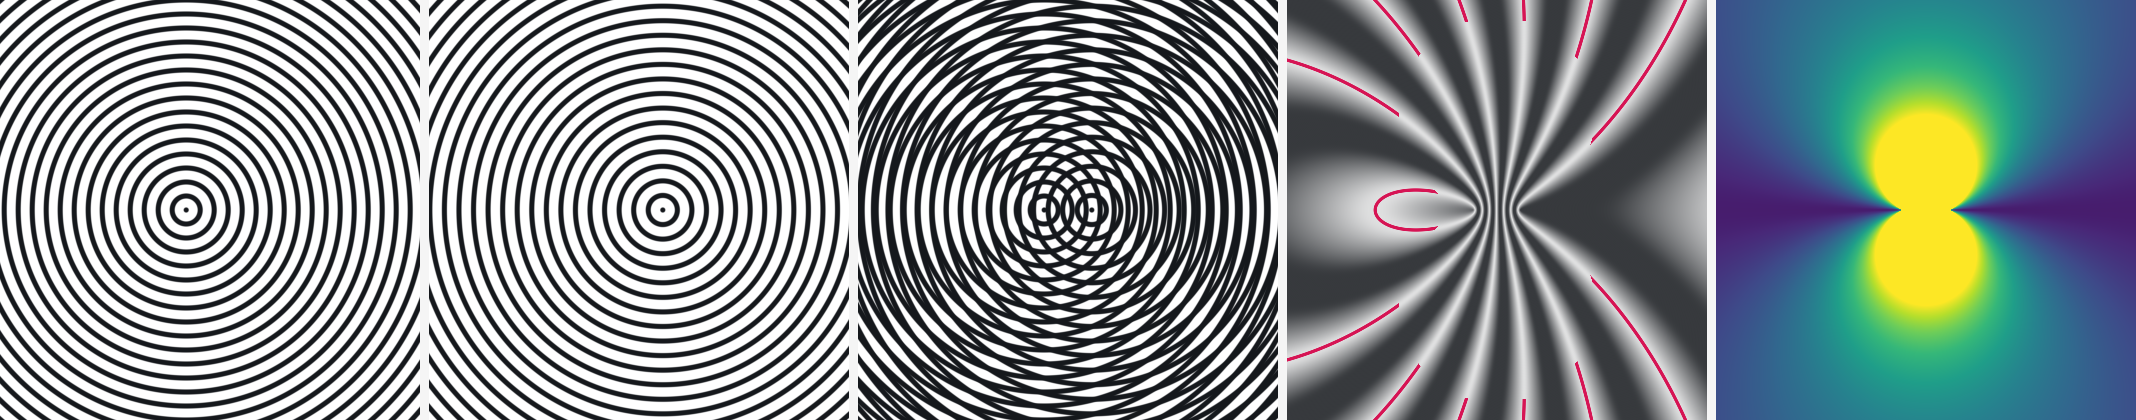
\includegraphics[width=\linewidth]{figures/fringe-law.png}
  \panelrow{0.19663}{0.00421}{%
    (a) layer $1$,
    (b) layer $2$,
    (c) superposition,
    (d) averaged ink\, $+\;\{D\in\Z\}$,
    (e) heterodyne ratio $\het$}
  \Description{Five square panels. The first two are black-on-white concentric rings
  about slightly different centres. The third overlays them and shows large curved
  bands cutting across the rings. The fourth is a smooth grey field of broad light
  and dark bands fanning out from the centre, its light bands traced by thin crimson
  curves that stop short of two blank lobes either side of centre. The fifth is a
  blue-to-yellow heat map of the same frame, dark blue over most of it with two
  bright yellow lobes where the crimson curves stopped.}
  \caption{\figlead{The moir\'e is a contour plot of the index difference.}
  \textbf{(a,\,b)} Two circle families, rendered alone from their own distance
  fields. Their centres differ by $34$ units and their pitches by four percent, and
  nothing else. \textbf{(c)} Their superposition, in which a fringe system appears
  that is in neither layer. \textbf{(d)} The theorem is a statement about averaged
  ink, so this is that average: the envelope view of \S\ref{sec:envelope}, which
  integrates the same two fields over one period of their common phase and so
  removes the carriers without blurring anything --- with the unit level sets of
  $D=\idx_1-\idx_2$ laid over it in crimson. Those curves are computed from the two
  index fields alone and never from the image, and they land on the light fringes.
  They are drawn only where
  $\het\le1/4$, which is why they stop short of the two lobes flanking the centres.
  \textbf{(e)} The heterodyne ratio $\het$ of Eq.~\ref{eq:ratio} over the same
  frame, dark where Theorem~\ref{thm:fringe} applies and bright where the two
  carriers are too different for a fringe to exist. The bright lobes are exactly the
  region the overlay declines to describe, and in the superposition they are exactly
  the region that reads as a rosette of crossings rather than as bands.}
  \label{fig:visibility}
\end{figure*}

We take $\het\le1/4$ as the operational definition of the fringe regime.

\subsection{Verification}

Theorem~\ref{thm:fringe} is a claim about a rendered image, so we measured it.
For ten scene pairs spanning straight, curved, isotropic, anisotropic, periodic and
aperiodic families, we compute the exact one-period directional mean of the union
from the fields themselves --- no raster, so no sampler error --- and compare it
against $\Phi$ evaluated at the window centre. There is no fitting and no free
parameter. Points are excluded on three stated grounds: strokes merged
($w_i+b_i>0.45$, so no gaps remain to beat), carrier bending more than $0.15$\,rad
across its own period, and gradient varying more than $15\%$ across a period, which
is the eikonal condition of Section~\ref{sec:eikonal}.

% GENERATED by paper/tools/numbers.mjs
\begin{table*}[t]
\caption{\figlead{The fringe law, measured.} Mean and $99$th-percentile absolute
error between the one-period directional mean of the rendered ink and $\Phi(D)$ of
Eq.~\ref{eq:phi}, over samples in the fringe regime $\het\le1/4$. \emph{Swing} is
the range of measured coverage, so it says how much fringe there was to get wrong.
\emph{Light\,/\,dark} are the mean distances of the measured lightest and darkest
deciles from the nearest integer index difference; the ideals are $0$ (light
fringes at $D\in\Z$) and $0.5$ (dark fringes at $D\in\Z+\tfrac12$). Where the
profile plateaus (low swing), the darkest decile spreads across the flat top and
its mean falls short of $0.5$ by construction. \emph{In regime} is the share of admissible samples with $\het\le1/4$. The
last row has none: with those settings no fringe exists, and the criterion says so
without rendering.}
\label{tab:fringe}
% The Families column carries long prose; \small leaves the widest row 11pt
% over the full text width, which prints into the margin.
\footnotesize
\centering
\begin{tabular}{@{}llrrrrcr@{}}
\toprule
Scene & Families & $n$ & mean & p99 & swing & light\,/\,dark & in regime \\
\midrule
\texttt{parallel-rotate} & two line families 6 degrees apart & 14,641 & 0.0000 & 0.0000 & 0.320 & 0.024 / 0.474 & 100\% \\
\texttt{parallel-pitch} & same direction, pitch mismatched by 4 percent & 14,641 & 0.0059 & 0.0189 & 0.326 & 0.026 / 0.470 & 100\% \\
\texttt{circle-circle} & circle families with displaced centres & 6,118 & 0.0000 & 0.0001 & 0.277 & 0.028 / 0.465 & 45\% \\
\texttt{circle-parallel} & circles under lines; D is not periodic in p & 3,952 & 0.0000 & 0.0000 & 0.242 & 0.034 / 0.475 & 27\% \\
\texttt{hexagon-hexagon} & anisotropic metric, hexagons 4 degrees apart & 13,382 & 0.0000 & 0.0000 & 0.260 & 0.024 / 0.475 & 95\% \\
\texttt{square-circle} & two different norms at the same spacing & 3,524 & 0.0000 & 0.0001 & 0.242 & 0.002 / 0.460 & 25\% \\
\texttt{spiral-circle} & aperiodic family: Archimedean spiral over circles & 14,041 & 0.0000 & 0.0001 & 0.243 & 0.031 / 0.461 & 100\% \\
\texttt{parabola-parabola} & curved families, bend mismatched by 8 percent & 484 & 0.0166 & 0.0329 & 0.169 & 0.160 / 0.218 & 100\% \\
\texttt{wave-parallel} & a wave family over lines & 14,641 & 0.0003 & 0.0011 & 0.118 & 0.011 / 0.170 & 100\% \\
\texttt{hyperbola-hyperbola} & rectangular hyperbolae, spacing mismatched by 4 percent & 11,036 & 0.0079 & 0.0214 & 0.640 & 0.123 / 0.430 & 100\% \\
\texttt{walking-circle} & a walking family (member $n$ displaced by $n\delta$) over concentric circles & 11,231 & 0.0159 & 0.0731 & 0.388 & 0.037 / 0.403 & 82\% \\
hyperbola\hspace{0.5pt}-\hspace{0.5pt}parallel & hyperbolae under lines: almost no fringe regime exists & --- & --- & --- & --- & --- & $0$ \\
\bottomrule
\end{tabular}
\end{table*}


Table~\ref{tab:fringe} reports the result. Across $\fringeSamples$ admissible
in-regime samples the mean absolute coverage error is $\fringeMeanErr$ and the
worst $99$th percentile over any scene is $\fringeWorstP$, against a fringe swing of
$0.24$--$0.64$ in coverage. The measured light fringes sit at mean index-gap
$\fringeLight$ from an integer and the dark fringes at $\fringeDark$ from a
half-integer, against ideals of $0$ and $0.5$.

The last row is the informative one. \texttt{hyperbola-parallel} has \emph{no}
in-regime samples anywhere in the frame: $\het>1/4$ everywhere, because a hyperbola
family's index gradient sweeps through all directions while a line family's does
not. There is no fringe in that superposition, only a lattice of crossings, and the
theory says so before rendering.

\section{The catalog}
\label{sec:catalog}

Section~\ref{sec:field} asked a layer for two things: a phase function $\ph$ whose
level sets are the members, and its gradient magnitude, which converts a phase
residual into a distance. This section is the list, and it is deliberately short:
thirteen families, of which nine are one line of algebra each. The four that
are not---the radial pencil and the three lattices---and the reason they
are not, set up the rest of the paper.
The supplemental material (\S S1) draws all thirteen, each alone and then beating
against a perturbed copy of itself, which is the fastest way to see what the
algebra below buys.

\subsection{Nine closed forms}

For a family whose members are $\{\ph=ns+\varphi\}$, the index and distance fields
of \S\ref{sec:field} are
\begin{equation}
  \idx(p)=\frac{\ph(p)-\varphi}{s},
  \qquad
  d(p)=\frac{\mathrm{periodicDist}\!\left(\ph(p)-\varphi,\,s\right)}{\lvert\nabla\ph(p)\rvert},
  \label{eq:closedpair}
\end{equation}
so a family is completely specified by the pair $(\ph,\lvert\nabla\ph\rvert)$.
Table~\ref{tab:catalog} gives both for all nine (ten rows: three are written-out instances of the $N$-gon). Every entry is $O(1)$, branch-free
apart from the free-side $N$-gon, and calls no transcendental function except where
the geometry genuinely contains an angle.

\begin{table*}[t]
  \centering
  \caption{\figlead{The nine phase families.} Each row is a complete
  specification: substitute $\ph$ and $\lvert\nabla\ph\rvert$ into
  \eqref{eq:closedpair} and the layer renders; the square, triangle and
  hexagon rows are the $N=4$, $3$, $6$ instances of the $N$-gon row, written
  out because their support forms are transcendental-free. $\omega=2\pi f/32$ so that
  $f=1$ is one wave cycle per $32$ world units; $a=B/100$ for a bend slider $B$;
  $b=Ms/2\pi$ with $M=\max(1,\mathrm{round}(\lvert B\rvert/s))$ the number of
  spiral arms. The three concentric shapes are the support function of the
  generating polygon, which is the observation \S\ref{sec:walking} builds on.}
  \label{tab:catalog}
  \small
  \begin{tabular}{@{}llll@{}}
    \toprule
    Family & $\ph(p)$ & $\lvert\nabla\ph(p)\rvert$ & Notes \\
    \midrule
    Parallel lines
      & $\langle p,u\rangle$
      & $1$
      & $u=(\cos\alpha,\sin\alpha)$; pitch $s$ \\
    Concentric circles
      & $\lVert p\rVert$
      & $1$
      & \\
    Concentric squares
      & $\max(\lvert x\rvert,\lvert y\rvert)$
      & $1$
      & $L^\infty$; support function of the square \\
    Concentric triangles
      & $\max\!\left(x,\ \tfrac{\sqrt3}{2}\lvert y\rvert-\tfrac{x}{2}\right)$
      & $1$
      & support function of the triangle \\
    Concentric hexagons
      & $\max\!\left(\lvert x\rvert,\ \tfrac{\lvert x\rvert}{2}+\tfrac{\sqrt3}{2}\lvert y\rvert\right)$
      & $1$
      & support function of the hexagon \\
    Concentric $N$-gon
      & $\lVert p\rVert\cos\!\big(\mathrm{wrap}(\theta_p,\tfrac{2\pi}{N})\big)$
      & $1$
      & $\theta_p=\mathrm{atan2}(y,x)$ \\
    Wave
      & $x-A\sin(\omega y+\ph_0)$
      & $\sqrt{1+A^2\omega^2\cos^2(\omega y+\ph_0)}$
      & $A$ amplitude, $f$ frequency, $\ph_0$ phase \\
    Parabola
      & $y-a x^2$
      & $\sqrt{1+4a^2x^2}$
      & opens up; $a=0$ is horizontal parallels \\
    Hyperbola
      & $\sqrt{\lvert x^2-y^2\rvert}$
      & $\lVert p\rVert/\sqrt{\lvert x^2-y^2\rvert}$
      & rectangular; $n\ge1$, so no member through $0$ \\
    Spiral
      & $\lVert p\rVert-b\,\theta_p$
      & $\sqrt{1+b^2/\lVert p\rVert^2}$
      & Archimedean; $b=0$ is concentric circles \\
    \bottomrule
  \end{tabular}
\end{table*}

Three remarks on the table; each marks a bug we shipped.

\paragraph{The gradient column is not decoration.} For the first six rows it is
$1$ and can be dropped. For the last four it is not, and dropping it thins every
stroke by the same factor the family is steep by. We had shipped that bug in
three of the four; \S\ref{sec:eikonal} reports the measurement.

\paragraph{Some families exclude an index.} The hyperbola's $n=0$ member would be
the degenerate pair $x=\pm y$, and $\lvert\nabla\ph\rvert$ blows up there, so the
family starts at $n=1$. The spiral's $\ph$ has a branch cut wherever
$\mathrm{atan2}$ does; it closes only if the arm count $M$ is an integer, which is
why $M$ is rounded rather than passed through. Both are the kind of detail that a
raster pipeline hides in the resampling and a field pipeline exposes on the
first frame.

\paragraph{Three of the rows are support functions.} The square, triangle and
hexagon entries are all $\rad(q)=\max_k\langle q,n_k\rangle$ over the outward
facet normals, written out. So is the $N$-gon row, in its trigonometric form. This
is not a coincidence and it is not only a way to avoid an $\mathrm{atan2}$:
\S\ref{sec:walking} shows that the same object supplies the constants that make
the hard case tractable.

\subsection{Four families that are not phase functions}

\paragraph{The radial pencil.} $N$ undirected lines through the layer origin,
equally spaced over $\pi$. There is no $\ph$ here whose level sets are the members:
the index winds around the origin, so any candidate phase is circle-valued with
a winding-number obstruction at the core---a phase singularity in the sense of
Nye and Berry~\cite{Nye1974Dislocations}---and admits no global scalar lift.
What the family does have is a distance,
\begin{equation}
  d(p)=\max\!\Big(\lVert p\rVert\,\big\lvert\sin\mathrm{wrap}(\theta_p,\tfrac{\pi}{N})\big\rvert,
  \;\; \varphi-\lVert p\rVert\Big),
  \label{eq:radial}
\end{equation}
which is what the renderer needs (here and in Table~\ref{tab:catalog},
$\mathrm{wrap}(v,w)$ maps $v$ into $[-w/2,w/2)$; the formula is exact except
in the corner wedge where a line meets the opened disc, where it understates
the distance to the trimmed member by a bounded factor), and an index---the
angular sector $\lfloor \theta_p N/\pi\rfloor$---which is what the fringe
law needs. The second
term is the parameter the interface calls \emph{Start}: it opens a disc of radius
$\varphi$ around the origin, because $N$ lines crossing at a point is a black dot,
and opening the center is the standard fix. Because the sector index is piecewise
constant in $\theta_p$ rather than smooth, a pencil against a pencil does not
produce fringes in the sense of Theorem~\ref{thm:fringe}; it produces the rosettes
that the classical literature treats separately~\cite{Amidror2009Theory}.

\paragraph{Lattices.} Square, hexagonal and triangular lattices index their
members by \emph{two} integers, not one. The nearest lattice point is found by
rounding in the lattice basis---for the hexagonal and triangular cases, cube
rounding on $(u,v,-u-v)$, the $A_2$ closest-point rule of Conway and
Sloane~\cite{Conway1982Fast}, exact and branch-light---and the layer offers
two distances from the result: to the nearest vertex, and to the nearest edge. The
hexagonal edge distance is again a support form, $\min_k(\mathrm{apothem}-\langle
q,n_k\rangle)$ over the six sides, so hexagon edges are hexagon sides and not
three superposed line families; getting this wrong produces a plausible-looking
pattern with the wrong symmetry. Both distances take an anisotropic scale
$(s_x,s_y)$, applied by dividing by $\lVert(n_x/s_x,n_y/s_y)\rVert$ per facet so
that stretching a lattice keeps its strokes metrically correct.

The consequence for the theory is plain. Theorem~\ref{thm:fringe}
is about the difference of two \emph{scalar} index fields. A lattice's index is in
$\Z^2$, so the difference of two lattice indices is in $\Z^2$ as well, and the
theorem applies to it componentwise---once per generating line family. This is
the classical situation, where a $2$-D screen superposition has a fringe
system per pair of generating frequency vectors and the visible moir\'e is whichever
pair beats slowest~\cite{Amidror2009Theory, Amidror1998Fourier}. The field
formulation does not remove that bookkeeping. It localizes it: each component is a
scalar field we can evaluate, difference, and map.

\subsection{A family with no closed-form index}

Take any of the concentric rows of Table~\ref{tab:catalog} and give member $n$ its
own rigid motion---displace it by $n\delta$, turn it by $n\theta$. The picture is
still a family of nested shapes, the parameters are two sliders, and the result is
the geometry of much op art. But $\ph$ is gone: each member now lives in
its own frame, so no closed-form expression in $p$ has these curves as its level
sets. An index field still exists implicitly wherever consecutive members bracket
the point (\S\ref{sec:fringe}), which is why the fringe law still applies; what is
lost is the formula, so the nearest index must be searched for.

That is the subject of the next two sections, and it is where the field view stops
being a change of notation and starts costing something.

\section{Folds: walking families}
\label{sec:walking}

The last rung of \S\ref{sec:taxonomy} is a count with no formula at all. This
section constructs the families that live there and the field they induce; the
next inverts them with a certificate. The tool that makes both tractable is
the same object the catalog's concentric rows were quietly built from.

\subsection{Radial metrics are support functions}

Fix a convex body $K\subset\R^2$ that is symmetric under rotation by $2\pi/N$ and
contains the origin. Write
\begin{equation}
  \rad(q) \;=\; \max_{u \in U}\, \langle q, u\rangle,
  \label{eq:support}
\end{equation}
where $U$ is the set of outward unit normals of $K$'s boundary. Then
$\rad(q)=R$ is precisely the boundary of the copy of $K$ with inradius $R$, so
$\rad$ is the natural ``radius'' for that shape. Equation~\eqref{eq:support} says
$\rad$ is the support function of $\mathrm{conv}(U)$~\cite{Rockafellar1970Convex}, and
the four cases our renderer exposes are all instances of it:
\begin{align}
  \text{circle:}\quad   &\rad(q) = \lVert q\rVert          &  U &= S^1, \notag\\
  \text{square:}\quad   &\rad(q) = \max(|q_x|, |q_y|)      &  U &= \{\pm e_1, \pm e_2\}, \notag\\
  \text{triangle:}\quad &\rad(q) = \max\Bigl(q_x,\; \tfrac{\sqrt3}{2}|q_y| - \tfrac{1}{2}q_x\Bigr), \notag\\
  \text{hexagon:}\quad  &\rad(q) = \max\Bigl(|q_x|,\; \tfrac{1}{2}|q_x| + \tfrac{\sqrt3}{2}|q_y|\Bigr).
  \label{eq:metrics}
\end{align}
The polygon forms in~\eqref{eq:metrics} are the max over $N$ unit normals written
out and folded by symmetry; for a free side count we evaluate
$\lVert q\rVert\cos(\mathrm{wrap}(\arg q, 2\pi/N))$ instead, which is the same
function. That the common cases avoid transcendentals entirely matters later:
$\rad$ is the innermost call of the solver.

We will use four properties, all immediate from~\eqref{eq:support}.

\begin{enumerate}
  \item[(P1)] \textbf{$1$-Lipschitz.} $|\rad(a)-\rad(b)| \le \lVert a-b\rVert$,
  since $U$ lies in the unit circle. This holds across corners, where $\nabla\rad$
  jumps.
  \item[(P2)] \textbf{Anisotropy floor.}
  $\kappa\lVert q\rVert \le \rad(q) \le \lVert q\rVert$ with
  \begin{equation}
    \kappa \;=\; \min_{\lVert v\rVert=1}\rad(v) \;=\; \cos(\pi/N),
    \label{eq:kappa}
  \end{equation}
  the inradius of $\mathrm{conv}(U)$: $1$ for the circle, $1/\sqrt2$ for the
  square, $1/2$ for the triangle. Both constants in~\eqref{eq:kappa} are attained,
  so neither can be improved.
  \item[(P3)] \textbf{Homogeneity and subadditivity.} $\rad(tq)=t\rad(q)$ for
  $t\ge0$ and $\rad(a+b)\le\rad(a)+\rad(b)$. Note that $\rad$ is \emph{not}
  symmetric: $\rad(-q)\neq\rad(q)$ for the triangle. This asymmetry is exactly
  what makes the drift constant of Section~\ref{sec:drift} directional.
  \item[(P4)] \textbf{Piecewise linearity.} For a polygon, $\rad$ is a max of $N$
  linear forms, hence convex and piecewise linear with $N$ pieces.
\end{enumerate}

\subsection{The family, and the field it induces}

\begin{figure}[t]
  \centering
  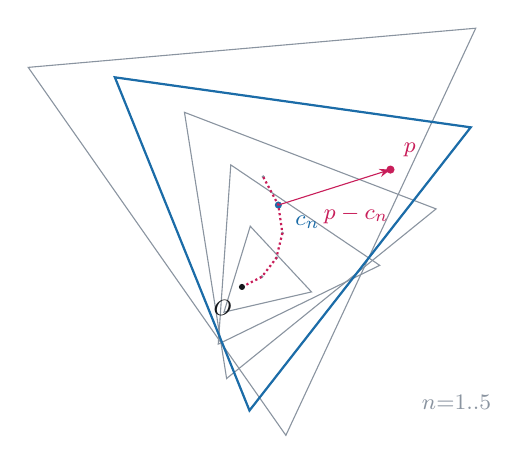
\begin{tikzpicture}[scale=0.92]
    % `\sp` is the inradius step, which is what the caption calls s. An equilateral
    % triangle's circumradius is twice its inradius; the factor here used to be
    % 1/cos(pi/6), which is the conversion for a *hexagon*, so the drawn triangles
    % were smaller than their stated inradius by 1/sqrt(3). The step is set so the
    % drawing is the size it always was, now under the right name.
    \def\sp{0.358}
    \def\dx{0.30}
    \def\dy{0.075}
    \def\th{13}
    % rings
    \foreach \n [evaluate=\n as \rr using 2*\n*\sp] [evaluate=\n as \cx using \n*\dx*cos(\n*\th) - \n*\dy*sin(\n*\th)] [evaluate=\n as \cy using \n*\dx*sin(\n*\th) + \n*\dy*cos(\n*\th)] in {1,2,3,4,5} {
      \draw[soft, thin, rotate around={\n*\th:(\cx,\cy)}]
        (\cx,\cy) +(90:\rr) -- +(210:\rr) -- +(330:\rr) -- cycle;
      \fill[soft] (\cx,\cy) circle (0.7pt);
    }
    % highlight ring 4
    \pgfmathsetmacro{\rr}{2*4*\sp}
    \pgfmathsetmacro{\cx}{4*\dx*cos(4*\th) - 4*\dy*sin(4*\th)}
    \pgfmathsetmacro{\cy}{4*\dx*sin(4*\th) + 4*\dy*cos(4*\th)}
    \draw[cool, thick, rotate around={4*\th:(\cx,\cy)}]
      (\cx,\cy) +(90:\rr) -- +(210:\rr) -- +(330:\rr) -- cycle;
    \fill[cool] (\cx,\cy) circle (1.4pt);
    \node[cool, font=\footnotesize, anchor=west] at (\cx+0.1,\cy-0.24) {$c_n$};
    % center walk
    \draw[accent, densely dotted, thick] (0,0)
      \foreach \n in {1,...,5} { -- ({\n*\dx*cos(\n*\th) - \n*\dy*sin(\n*\th)}, {\n*\dx*sin(\n*\th) + \n*\dy*cos(\n*\th)}) };
    \fill[ink] (0,0) circle (1.2pt);
    \node[ink, font=\footnotesize, anchor=north east] at (0,-0.05) {$O$};
    % query point. The arrow is drawn in world coordinates, so it is p - c_n; the
    % pulled-back point q_n is that same vector read in ring n's own frame, which
    % is a different vector, and rho is not rotation invariant -- labelling this
    % arrow q_n would undercut the very thing the figure is about.
    \coordinate (P) at (2.05,1.62);
    \fill[accent] (P) circle (1.6pt);
    \node[accent, font=\footnotesize, anchor=south west] at (2.1,1.66) {$p$};
    \draw[accent, thin, -{Stealth[length=4pt]}] (\cx,\cy) -- (P);
    \node[accent, font=\footnotesize] at (1.58,1.0) {$p-c_n$};
    \node[soft, font=\footnotesize, anchor=west] at (2.35,-1.6) {$n{=}1..5$};
  \end{tikzpicture}
  \Description{A diagram of five nested triangles of increasing size, each rotated a
  little further than the last and each centered a little further from the origin, so
  their centers trace a short dotted spiral outwards. The fourth triangle and its
  center are picked out in blue and labeled, and an arrow runs from that center to a
  query point marked inside the fourth triangle.}
  \caption{A walking family of triangles ($N=3$), drawn with $\varphi=0$. Ring $n$
  has inradius $ns+\varphi$, its center $c_n = \Rot{n\theta}(n\delta)$ walks along
  the dotted spiral, and its own frame is turned by $n\theta$. Rendering asks for
  the distance from $p$ to the nearest ring; the residual of ring $n$ is measured
  in that ring's frame, on the pulled-back point
  $q_n = \Rot{-n\theta}\,p - n\delta = \Rot{-n\theta}(p - c_n)$. The arrow is
  $p-c_n$, which is that same displacement in world coordinates: the two have equal
  length, but $\rad$ is not rotation invariant, so it is $q_n$ and not the arrow
  that the residual is taken of. That is the difficulty in one picture: because
  each ring has a different frame, no closed-form scalar field of $p$ has these
  rings as its level sets, and the index field survives only as the answer to a
  search (\S\ref{sec:inverse}).}
  \label{fig:family}
\end{figure}

A \emph{walking family} is the sequence of curves
\begin{equation}
  \Gamma_n \;=\; \bigl\{\, p : \rad\bigl(\Rot{-n\theta}(p - c_n)\bigr) = ns+\varphi \,\bigr\},
  \qquad c_n = \Rot{n\theta}(n\delta),
  \label{eq:family}
\end{equation}
for $n\in\N_0$, with spacing $s>0$, phase $\varphi\ge0$ (so that every radius
$ns+\varphi$ is nonnegative), per-index translation
$\delta\in\R^2$, and per-index rotation $\theta$. Figure~\ref{fig:family} shows
one. The three degenerate cases are familiar: $\delta=0,\theta=0$ gives
concentric shapes; $\theta=0$ alone gives a family whose centers walk a straight
line; and degenerating the shape to a half-plane, whose support set $U$ is a
single normal, recovers parallel lines at spacing $s$.

Expanding $\Rot{-n\theta}(p - \Rot{n\theta}(n\delta))$ gives the pulled-back
point
\begin{equation}
  q_n(p) \;=\; \Rot{-n\theta}\,p \;-\; n\delta,
  \label{eq:qn}
\end{equation}
which is the form we compute with: a rotation of $p$ that advances by $\theta$ per
index, minus a translation that advances by $\delta$ per index. Define the
\emph{index residual}
\begin{equation}
  h_p(n) \;=\; \rad\bigl(q_n(p)\bigr) - (ns + \varphi),
  \label{eq:residual}
\end{equation}
positive when $p$ falls outside ring $n$ and negative when inside. The distance
field the renderer wants is
\begin{equation}
  d(p) \;=\; \min_{n\in\N_0} \bigl|h_p(n)\bigr|.
  \label{eq:field}
\end{equation}
This is not the Euclidean distance to $\Gamma_{n^\star}$; it is the residual of
the inradius metric, which agrees with Euclidean distance for circles and
\emph{under}estimates it for polygons, by a factor of at most $1/\kappa$:
(P1) gives residual $\le$ distance always, and the gauge comparison gives
distance $\le$ residual$/\kappa$. Renderers of this kind consume $d$ through a
smoothstep of width one pixel, so the distinction thickens apparent stroke
weight near corners and changes nothing else. We keep the metric residual
because it is what admits the bounds below; the Limitations of
Section~\ref{sec:discussion} note the cost.

\subsection{The inversion problem}

Equation~\eqref{eq:field} is a minimization over an infinite discrete set, so
every practical solver is an argument about which finitely many $n$ can be
skipped. Three regimes are classical and one is not.

When $\delta=0$ and $\theta=0$, $h_p(n) = \rad(p)-ns-\varphi$ is affine in $n$,
so $d(p) = \mathrm{dist}\bigl((\rad(p)-\varphi) \bmod s\bigr)$ exactly: one
evaluation. When the shape is a circle and $\theta=0$, $\lVert p - n\delta\rVert =
ns+\varphi$ is a quadratic in $n$ whose roots bracket the answer; two integer
evaluations suffice. When $\theta=0$ and the shape is a polygon, $h_p$ is convex
and piecewise linear; we give the exact solution in
Section~\ref{sec:closed}. We have not found it stated elsewhere, and its
marginal case is the part that matters in practice.

Everything else (any $\theta\neq0$) has no closed form, because $q_n$ in
\eqref{eq:qn} contains $\Rot{-n\theta}p$, and asking for $h_p(n)=0$ asks where a
sinusoid in $n$ meets a line in $n$. That is transcendental, with a solution count
that depends on the parameters. The question is therefore not how to solve it, but
how few integers we can prove it suffices to test.

The naive answer is $n \approx \rad(p)/s$, ``the ring whose radius matches the
pixel's radius,'' plus a fixed number of neighbors. The next section shows how
far that can be from the truth, and replaces it with a provably sufficient
interval.

\section{Bounded inversion}
\label{sec:inverse}

\subsection{The guard}
\label{sec:guard}

The solver does not need $d(p)$ everywhere. Coverage is computed as
$1-\mathrm{smoothstep}(h-a,\,h+a,\,d)$ for stroke half-width $h$ and
antialiasing width $a$ (Eq.~\ref{eq:alpha}), so any $d$ above $h+a$ produces
identical output. We therefore fix a \emph{guard}
\begin{equation}
  G \;=\; \max\bigl(h+a,\ \tfrac{3}{4}s\bigr)
  \label{eq:guard}
\end{equation}
and require only
\begin{equation}
  \tilde d(p) \;=\; \min\bigl(d(p),\, G\bigr).
  \label{eq:clamped}
\end{equation}
Everything below is exact with respect to~\eqref{eq:clamped}, which is exact with
respect to the image: the clamp is the renderer's own quantization, and it
changes no output pixel. (The envelope and ratio views of
\S\ref{sec:envelope}--\S\ref{sec:visibility} need the field measured a whole
pitch out rather than a stroke width out, so under those views the solver runs
with $G$ widened to $\max(h+a,\,s)$; every bound below holds verbatim at the
wider value.)

Two smaller consequences of the same observation come free. The solver takes an
\emph{accept} threshold $h-a$: once a residual falls
below it the pixel is fully inked and the loop can stop, whatever else is nearby.
And it takes $G$ itself as a \emph{reject} threshold, which is what makes the
interval below finite.

\subsection{The drift constant}
\label{sec:drift}

Everything turns on how fast ring $n$'s boundary can outrun its own radius. Using
(P3) on~\eqref{eq:qn},
\begin{equation}
  \rad(q_n) \;=\; \rad\bigl(\Rot{-n\theta}p - n\delta\bigr)
    \;\le\; \rad\bigl(\Rot{-n\theta}p\bigr) + n\,\rad(-\delta),
  \label{eq:driftup}
\end{equation}
so the per-index rate is exactly
\begin{equation}
  m \;=\; \rad(-\delta),
  \label{eq:drift}
\end{equation}
the support value of the metric in the direction \emph{opposite} the walk. The
obvious bound is $m \le \lVert\delta\rVert$, and $\lVert\delta\rVert$ is what a
first implementation naturally uses. But~\eqref{eq:drift} is smaller, sometimes
much smaller: $m=\max(|\delta_x|,|\delta_y|)$ for a square, and as little as
$\lVert\delta\rVert/2$ for a triangle whose flat side leads the walk (the
vertex trailing); with the vertex leading, $m=\lVert\delta\rVert$ and nothing
is gained.

The same number has a physical face: Corollary~\ref{cor:mach} says the family
folds exactly when $m>s$, so $m$ is the Mach number of the walk, and the
solver constants below are the search-side shadow of the fold law.

The gap is not cosmetic. Section~\ref{sec:window} shows the search interval is
finite if and only if $m \neq s$, with width $\propto 1/|s-m|$. Substituting
$\lVert\delta\rVert$ for $m$ therefore declares an entire band of settings
unbounded that are in fact tightly bounded, and a solver that falls back to
subsampling on that band produces the failure in Figure~\ref{fig:drift}: not holes,
but a wholesale thinning that removes two thirds of the ink and looks, to a user,
like the pattern has changed. It is the largest single fidelity error we measured
from any cause ($\artDriftLooseDiff\%$ of pixels), and it comes from a bound that
is merely loose rather than wrong.

\subsection{A provably sufficient interval of indices}
\label{sec:window}

\begin{figure*}[t]
  \centering
  \begin{subfigure}[t]{0.485\textwidth}
    \vspace{0pt}
    \begin{tikzpicture}
      \begin{axis}[paperaxis, scale only axis, width=6.4cm, height=4.2cm, name=resax,
        xlabel={ring index $n$}, ylabel={residual $h_p(n)$},
        xmin=0, xmax=74, ymin=-260, ymax=380,
        legend style={at={(0.5,-0.36)}, anchor=north, draw=none, fill=none,
                      /tikz/every even column/.append style={column sep=0.45cm}},
        legend columns=2,
      ]
        % window shading
        \addplot[draw=none, fill=cool!10, forget plot] coordinates
          {(\figLo,-260) (\figHi,-260) (\figHi,380) (\figLo,380)} \closedcycle;
        % guard band
        \addplot[draw=none, fill=accent!22, forget plot] coordinates
          {(0,-10.5) (74,-10.5) (74,10.5) (0,10.5)} \closedcycle;
        \addplot[cool, thick, dashed] table [x=n, y=upper, col sep=comma] {data/residual.csv};
        \addlegendentry{upper envelope $r + n(m-s)$}
        \addplot[warm, thick, dashed] table [x=n, y=lower, col sep=comma] {data/residual.csv};
        \addlegendentry{lower envelope $\kappa|r-nL| - ns$}
        \addplot[ink, very thick] table [x=n, y=h, col sep=comma] {data/residual.csv};
        \addlegendentry{$h_p(n)$}
        \addplot[only marks, mark=*, mark size=1.9pt, accent]
          table [x=n, y=h, col sep=comma] {data/residual-visited.csv};
        \addlegendentry{evaluated (\figEvals)}
        \draw[soft, dashed] (axis cs:\figNaive,-260) -- (axis cs:\figNaive,380);
        \node[soft, font=\scriptsize, anchor=south, rotate=90] at (axis cs:\figNaive,-250) {naive $r/s$};
      \end{axis}
      \path ([yshift=8pt]resax.north);
    \end{tikzpicture}
    \caption{The residual at one pixel.}
    \label{fig:residual}
  \end{subfigure}\hfill
  \begin{subfigure}[t]{0.485\textwidth}
    \vspace{0pt}
    \begin{tikzpicture}
      \begin{axis}[paperaxis, scale only axis, width=6.4cm, height=4.2cm, name=fanax,
        xlabel={$\lVert p\rVert$ (world units, $s=14$)}, ylabel={indices},
        xmin=0, xmax=1600, ymin=0, ymax=82,
        legend style={at={(0.5,-0.36)}, anchor=north, draw=none, fill=none,
                      /tikz/every even column/.append style={column sep=0.45cm}},
        legend columns=2,
      ]
        \addplot[accent, very thick] table [x=radius, y=stray, col sep=comma] {data/fan-triangle.csv};
        \addlegendentry{worst stray of $n^\star$}
        \addplot[cool, thick, densely dashed] table [x=radius, y=span, col sep=comma] {data/fan-triangle.csv};
        \addlegendentry{proven interval}
        \addplot[warm, thick] table [x=radius, y=evaluated, col sep=comma] {data/fan-triangle.csv};
        \addlegendentry{indices we evaluate}
        \addplot[soft, thin, dotted, domain=0:1600, samples=2] {16};
        \addlegendentry{$\pm16$ budget}
      \end{axis}
      \path ([yshift=8pt]fanax.north);
    \end{tikzpicture}
    \caption{Worst-case stray against radius.}
    \label{fig:fan}
  \end{subfigure}
  \Description{Two plots. The left plots the residual against ring index: a steeply
  falling dark curve crosses zero near index forty-one, bracketed above and below by
  two dashed straight lines, with a pink horizontal guard band around zero and a
  shaded vertical strip marking the certified index interval; nine dots on the curve
  mark the indices actually evaluated, widely spaced far from the crossing and
  closely spaced near it. The right plots four quantities against radius: the worst
  stray of the nearest index grows roughly linearly past sixty, the proven interval
  width grows with it, the count of indices evaluated stays near ten, and a dotted
  horizontal line at sixteen marks a fixed budget that the stray crosses early.}
  \caption{\figlead{Certifying and skipping the index interval.}
  \textbf{(a)}~The residual at one pixel is sandwiched between two lines in $n$,
  which is enough to certify a finite interval. The naive index guess is
  $\figNaive$; the true nearest ring is $\figTrue$, $\figGap$ rings away and
  outside any small neighborhood. The two envelopes of Lemma~\ref{lem:envelope}
  cross the guard band (pink) at $\figLo$ and $\figHi$, proving that no ring
  outside those $\figSpan$ indices comes within $G$; the Lipschitz rule then
  visits $\figEvals$ of them (dots), taking long strides while $|h|$ is large
  and closing in only near the crossing. \textbf{(b)}~Why no fixed interval
  could have been enough, measured. Triangles, $\theta=0.02$, $96$ directions
  per radius; the stray is the worst seen out to that radius. The nearest index
  leaves any fixed neighborhood of the naive guess and the gap grows linearly,
  so a budget is a horizontal line that the requirement crosses, here at
  $r\approx500$, a third of the way across the frame. The proven interval grows
  too, since the rings near a pixel genuinely become more numerous, but the
  Lipschitz skip keeps what we evaluate well below it.}
  \label{fig:bounds}
\end{figure*}

Write $r=\lVert p\rVert$, $L=\lVert\delta\rVert$, $m=\rad(-\delta)$, and note
$\rad(\Rot{-n\theta}p)\le r$ by (P2) and
$\lVert q_n\rVert \ge |r - nL|$ by the triangle inequality on~\eqref{eq:qn};
both are independent of $\theta$.

\begin{lemma}[Two-sided envelope]
\label{lem:envelope}
For all $n \ge 0$ and all $\theta$,
\begin{equation}
  \max\bigl\{\, \kappa\,|r - nL|,\ \ nm - r \,\bigr\} - (ns+\varphi)
  \ \le\ h_p(n)\ \le\ r + nm - (ns+\varphi).
  \label{eq:envelope}
\end{equation}
\end{lemma}

\begin{proof}
The upper bound is~\eqref{eq:driftup} with $\rad(\Rot{-n\theta}p)\le r$. For the
first lower bound, (P2) gives $\rad(q_n) \ge \kappa\lVert q_n\rVert \ge
\kappa|r-nL|$. For the second, subadditivity applied as
$\rad(-n\delta) \le \rad(q_n) + \rad(-\Rot{-n\theta}p)$ gives
$\rad(q_n) \ge nm - r$. Subtract $ns+\varphi$ throughout.
\end{proof}

Both bounds are affine in $n$ (the first piecewise so), so intersecting them with
the guard band $|h|\le G$ yields an interval by inspection.

\begin{theorem}[Sufficient interval]
\label{thm:window}
Let
\begin{equation}
  n_{\mathrm{lo}} = \max\left(0,\ \left\lfloor \frac{\kappa r - \varphi - G}{s + \kappa L} \right\rfloor\right),
  \qquad
  n_{\mathrm{hi}} = \left\lceil \frac{r + \varphi + G}{|s - m|} \right\rceil .
  \label{eq:window}
\end{equation}
If $m \neq s$, then every $n$ with $|h_p(n)| \le G$ satisfies
$n_{\mathrm{lo}} \le n \le n_{\mathrm{hi}}$, and consequently
\begin{equation}
  \tilde d(p) \;=\; \min\Bigl(G,\ \min_{n_{\mathrm{lo}} \le n \le n_{\mathrm{hi}}} |h_p(n)|\Bigr).
  \label{eq:exact}
\end{equation}
\end{theorem}

\begin{proof}
For the lower end, note first that every $n < n_{\mathrm{lo}}$ lies on the
branch $nL\le r$ automatically: $n(s+\kappa L) < \kappa r - \varphi - G \le
\kappa r$ gives $\kappa nL < \kappa r$. On that branch \eqref{eq:envelope}
gives $h_p(n) \ge \kappa r - \kappa nL - ns - \varphi > G$, so
$|h_p(n)| > G$ and no index below $n_{\mathrm{lo}}$ is admitted. For the upper
end, if $s>m$ then $h_p(n) \le r + n(m-s) - \varphi$, and $h_p(n)\ge -G$ forces
$n \le (r - \varphi + G)/(s-m)$; if $m>s$ then $h_p(n) \ge n(m-s) - r - \varphi$,
and $h_p(n)\le G$ forces $n \le (r + \varphi + G)/(m-s)$. Both are bounded
by~\eqref{eq:window}. Every excluded index has $|h_p(n)|>G$, so it cannot lower
the clamped minimum, giving~\eqref{eq:exact}.
\end{proof}

Three remarks. First, \emph{$\theta$ does not appear} in~\eqref{eq:window}. The
rotation destroys the closed form but does not widen the search: it is bounded
away by $\rad(\Rot{-n\theta}p)\le r$, which is tight since some index does place
$p$ along a vertex direction. Second, the interval is tight in the sense that both
envelope constants are attained, so it cannot be narrowed without using more than
$\rad$'s convexity class. Third, the interval degenerates only on the single locus
$m=s$: there, the two envelopes are parallel to the guard band and infinitely many
rings genuinely pass within $G$ of a generic point. That is not a failure of the
bound but a property of the family, and we return to it in
Sections~\ref{sec:closed} and~\ref{sec:limits}.

Figure~\ref{fig:residual} works one pixel through. The naive guess is $\figNaive$;
the truth is $\figTrue$, $\figGap$ rings away. The proven interval is
$[\figLo,\figHi]$, and Figure~\ref{fig:fan} shows why no constant would have done:
we measured how far the nearest index actually strays from the naive guess, worst
case over directions, and it grows linearly in $r$: past $r\approx500$ it
exceeds the widest neighborhood our previous solver could even express. The same
plot confirms the theorem empirically: over $\winChecks$ sampled pixels whose
nearest ring is inside the guard, the argmin fell inside~\eqref{eq:window} every
time.

\subsection{Skipping the interval}
\label{sec:skip}

An interval is a proof, not yet an algorithm; near the origin it is a handful of
indices, but at zoom-out it can be thousands. We shrink it with a Lipschitz
argument in index space.

\begin{lemma}[Index Lipschitz bound]
\label{lem:lipschitz}
For all $n, n'\ge 0$,
$|h_p(n')-h_p(n)| \le \Lambda\,|n'-n|$ with
\begin{equation}
  \Lambda \;=\; s + L + |\theta|\,r .
  \label{eq:lambda}
\end{equation}
\end{lemma}

\begin{proof}
By (P1), $|\rad(q_{n'})-\rad(q_n)| \le \lVert q_{n'}-q_n\rVert$. From
\eqref{eq:qn}, $\lVert q_{n'}-q_n\rVert \le
\lVert(\Rot{-n'\theta}-\Rot{-n\theta})p\rVert + |n'-n|L
= 2r\bigl|\sin\tfrac{(n'-n)\theta}{2}\bigr| + |n'-n|L
\le |n'-n|\,(|\theta| r + L)$. The ring radius contributes $s|n'-n|$.
\end{proof}

So from a sample with residual $|h_p(n)| = v$ and a current best $b$, no index
within $(v-b)/\Lambda$ of $n$ can beat $b$, and the whole run can be skipped
unevaluated. This is sphere tracing~\cite{Hart1996Sphere} with the ray replaced by the
index axis. The loop is Algorithm~\ref{alg:scan}.

\begin{algorithm}[t]
\caption{Ring scan, given $p$, the family parameters, the budget $B$, the guard
$G$, and the accept threshold $h-a$. With
$\mathrm{span}=n_{\mathrm{hi}}-n_{\mathrm{lo}}+1$, exact when
$\mathrm{span}\le B$ (Theorem~\ref{thm:window}).}
\label{alg:scan}
\begin{algorithmic}[1]
\State $[n_{\mathrm{lo}}, n_{\mathrm{hi}}] \gets$ interval from \eqref{eq:window};
       $\Lambda \gets s + L + |\theta| r$
\State $\sigma \gets 2^{\max(0,\,\lceil \log_2(\mathrm{span}/B) \rceil)}$ \Comment{$1$ when the interval fits}
\State $n \gets \sigma\lceil n_{\mathrm{lo}}/\sigma \rceil$ \Comment{anchored to the global lattice, not to $p$}
\State carry $\cos(n\theta-\arg p)$, $\sin(n\theta-\arg p)$, $n\delta$, $ns+\varphi$
\State $b \gets \infty$
\For{$B$ iterations, while $n \le n_{\mathrm{hi}}$}
  \State $v \gets |\rad(q_n) - (ns+\varphi)|$ \Comment{no transcendentals}
  \State $b \gets \min(b, v)$
  \State \textbf{if} $b \le$ accept \textbf{then return} $b$
  \State $j \gets \sigma\max\bigl(1, \lceil (\lfloor (v - \min(b,G))/\Lambda \rfloor + 1)/\sigma \rceil\bigr)$
  \State advance the carried quantities by $j$; $n \gets n + j$
\EndFor
\State \Return $\min(b, G)$
\end{algorithmic}
\end{algorithm}

Two implementation points matter enough to measure (Table~\ref{tab:ablation}).

\emph{Carried motion.} $q_n$ advances by a fixed rotation and a fixed translation
per index, so the loop carries $\cos(n\theta-\arg p)$ and $\sin(n\theta-\arg p)$
through an angle-addition step instead of recomputing them. Combined with the
transcendental-free forms in~\eqref{eq:metrics}, the inner iteration contains no
transcendental function at all: it is a handful of multiplies, a max, and an
absolute value. We re-anchor every $32$ carried steps, which keeps
\texttt{f32} drift far below a pixel; at large $n$ the carried value is in fact steadier than
$\cos(n\theta-\alpha)$ evaluated cold, because the argument does not grow.

\emph{Lattice anchoring.} When the interval exceeds the budget $B$ we stride by a
power of two, and the start is snapped to a multiple of the stride rather than to
$n_{\mathrm{lo}}$. Since $n_{\mathrm{lo}}$ depends on $p$ and the stride does not,
this is the difference between neighboring pixels agreeing on \emph{which rings
exist} and each pixel sampling its own subset. Section~\ref{sec:limits} shows the
consequence, which is severe and free to avoid.

\subsection{Translated polygons in closed form}
\label{sec:closed}

\begin{figure}[t]
  \centering
  \begin{tikzpicture}
    \begin{axis}[paperaxis, height=5.3cm,
      xlabel={ring index $n$}, ylabel={$h_p(n)$},
      xmin=0, xmax=64, ymin=-700, ymax=440,
      ytick={-600,-400,-200,0,200,400},
      legend style={at={(0.5,-0.40)}, anchor=north, draw=none, fill=none,
                    /tikz/every even column/.append style={column sep=0.45cm}},
      legend columns=2,
    ]
      % Zero is a line, not a band: at this scale a band wide enough to see would
      % be wider than the crossing it marks.
      \addplot[accent, thin, forget plot] coordinates {(0,0) (64,0)};
      \addplot[cool, very thick] table [x=n, y=h, col sep=comma] {data/convex-shrinking.csv};
      \addlegendentry{$m < s$: one crossing}
      % Dashed, not for emphasis: the two residuals very nearly coincide until the
      % second facet, and a solid line drawn second would simply hide the first.
      \addplot[warm, very thick, densely dashed] table [x=n, y=h, col sep=comma] {data/convex-marginal.csv};
      \addlegendentry{$m = s$: flat forever}
      % Where one facet hands over to the next, from the same data the curves use.
      \addplot[cool, only marks, mark=*, mark size=1.5pt, mark options={fill=white, thick},
               forget plot] table [x=n, y=h, col sep=comma] {data/convex-shrinking-breaks.csv};
      \addplot[warm, only marks, mark=*, mark size=1.5pt, mark options={fill=white, thick},
               forget plot] table [x=n, y=h, col sep=comma] {data/convex-marginal-breaks.csv};
      \node[anchor=north east, inner sep=1.5pt, fill=white, draw=cool, semithick]
        at (rel axis cs: 0.615, 0.97) {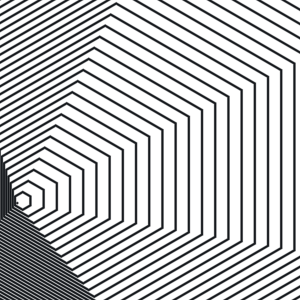
\includegraphics[width=1.62cm]{figures/inset-convex-cross.png}};
      \node[anchor=north east, inner sep=1.5pt, fill=white, draw=warm, semithick]
        at (rel axis cs: 0.985, 0.97) {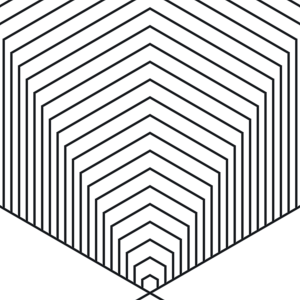
\includegraphics[width=1.62cm]{figures/inset-convex-flat.png}};
    \end{axis}
  \end{tikzpicture}
  \Description{A plot of the residual against ring index for two settings, with a
  thin horizontal line at zero. Both curves start near four hundred and fall. The
  blue curve is visibly made of four straight pieces of decreasing steepness, with
  small hollow circles where one piece meets the next; it crosses zero once, part
  way along its second piece, and keeps descending. The orange curve falls through
  three pieces and then levels onto a horizontal line, which it holds for the rest
  of the plot. Two small framed thumbnails at the top right show the two walking
  hexagon families the curves belong to.}
  \caption{With $\theta=0$ the residual of a translated polygon is convex and
  piecewise linear in $n$, one segment per facet (hexagon, $s=14$); the hollow
  circles mark the handovers. When the drift is below the spacing (blue, $m=10$)
  it falls monotonically and crosses zero once, on some facet's own segment, so
  the answer is a linear solve. At the marginal drift $m=s$ (orange) the leading
  facet's slope cancels and the residual is \emph{constant} past the crossover:
  all large indices are exactly equidistant, so no enumeration of finite length
  can settle them. One evaluation of the constant settles all of them at once.
  The insets are these same two families, framed in each curve's color: below the
  marginal drift the walking hexagons stay a drawing; at it the far side piles
  into a plateau. Both curves are shown on the query point of
  Table~\ref{tab:cost}'s hexagon setting; the point and the drift are deliberately
  not parallel, since a $p$ collinear with $\delta$ keeps one facet active for
  every $n$ and would draw a single straight line here.}
  \label{fig:convex}
\end{figure}

The scan of Algorithm~\ref{alg:scan} is exact and fast, but for $\theta=0$ the
scan can be replaced by an exact $O(N)$ solution regardless of the interval
width, including on the locus where the interval is infinite. Property (P4) is the reason,
and we have not found it used for this.

With $\theta=0$, \eqref{eq:qn} becomes affine in $n$: $q_n = p - n\delta$. Writing
$a_k = \langle p, u_k\rangle$ and $b_k = \langle \delta, u_k\rangle$ over the $N$
unit normals,
\begin{equation}
  h_p(n) \;=\; \max_{k}\,(a_k - n b_k) \;-\; ns - \varphi ,
  \label{eq:convex}
\end{equation}
a maximum of $N$ affine functions of $n$ minus an affine function: convex and
piecewise linear, with at most $N$ breakpoints and slopes increasing in $n$. Its
asymptotic slope is $m - s$ with $m=\rad(-\delta)=\max_k(-b_k)$: the same drift
constant as~\eqref{eq:drift}, arrived at independently.

\begin{proposition}
\label{prop:closed}
Let $\theta=0$, let the shape be a polygon with $N$ facets, and let $p$ lie on
or outside the innermost ring, $\rad(p)\ge\varphi$. (Inside it, $h_p$ is
negative and strictly decreasing, so the answer is
$\min(G,\,\varphi-\rad(p))$, attained at $n=0$.)
\begin{enumerate}
  \item If $m < s$, $h_p$ is strictly decreasing and has exactly one zero, which
  lies on some facet's own linear segment. That zero is one of the $N$ solves
  $n_k = (a_k-\varphi)/(s+b_k)$, and
  $\tilde d(p) = \min(G,\min_k \min_{j\in\{\lfloor n_k\rfloor, \lfloor n_k\rfloor+1\}} |h_p(j)|)$,
  with each candidate clamped to $j\ge0$: an unclamped negative candidate
  indexes a ring that does not exist.
  \item If $m = s$, the facet $k^\star$ attaining $m$ has $s + b_{k^\star} = 0$
  (its solve is skipped), and $h_p \equiv a_{k^\star} - \varphi$ on the terminal
  segment, attained at every index past the crossover. $\tilde d(p)$ is the
  minimum of $|a_{k^\star}-\varphi|$ against the remaining facets' clamped
  candidates as in (1), then clamped at $G$.
\end{enumerate}
In both cases the cost is $2N+2$ evaluations of~\eqref{eq:convex}, independent of
$r$, $s$, and $\delta$.
\end{proposition}

\begin{proof}
By~\eqref{eq:convex} $h_p$ is convex with slopes $-(s+b_k)$ ordered increasingly
in $n$. If $m<s$ then $s + b_k > 0$ for every $k$, so every slope is negative and
$h_p$ is strictly decreasing; being continuous with $h_p(0)=\rad(p)-\varphi\ge0$
by hypothesis and $h_p\to-\infty$, it has one zero, attained
on whichever segment is active there, whose linear equation is
$a_k - nb_k - ns - \varphi = 0$. Convexity makes $|h_p|$ unimodal, so its integer
minimum is adjacent to the real zero. If $m=s$, the maximum in~\eqref{eq:convex}
is eventually attained by $k^\star$, and there
$h_p(n) = a_{k^\star} + ns - ns - \varphi$ is constant; before the crossover
$h_p$ is a strictly decreasing piecewise-linear function whose zero, if it has
one, is covered by the remaining facets' candidates.
\end{proof}

The square case ($N=4$, normals on the axes) is presumably folklore; the content
of Proposition~\ref{prop:closed} is that it generalizes to every side count
and, more importantly, that case (2) exists.
Figure~\ref{fig:convex} plots both. The marginal case is the one that repays the
effort: it is exactly the locus where Theorem~\ref{thm:window} gives up, it is
the sonic boundary of Corollary~\ref{cor:mach} --- the walk that matches its
own growth, rings piling into a plane wake --- and it is
not exotic. It is the family whose rings pile up along a line, which is a
pattern users deliberately make. Any scan, of any budget, walks off the end of
that flat segment without reaching the indices that carry the answer. Handling it
costs one comparison. Table~\ref{tab:ablation} measures the difference at
$\ablClosedMarginal\times$.

We dispatch to the cheapest sufficient method: constant-time \texttt{mod} when
$\delta=0$ and ($\theta=0$ or the shape is a circle, since rotating a radial
metric is a no-op --- for circles alone, by
Corollary~\ref{cor:rotation}); the quadratic for translated circles; Proposition~\ref{prop:closed}
for translated polygons with integral side count and $m \le s$;
Algorithm~\ref{alg:scan} otherwise. A morph that passes through fractional side
counts is not any polygon's support function, so it correctly falls through to the
scan rather than solving for facets that do not exist.

\subsection{Implementation}
\label{sec:impl}

The solver exists twice: once in TypeScript for tests and once in WGSL for the
renderer, generated as separate functions and composed as shader
includes~\cite{WebGPU}. The twins are checked against each other numerically on
the GPU (Section~\ref{sec:protocol}) and the TypeScript side is checked against
brute force in a unit test that sweeps shapes, spacings, offsets, and radii,
including the marginal drift. Ring evaluation is branch-light: the interval, the
stride, and $\Lambda$ are computed once per pixel, and the loop body has a single
data-dependent branch (the accept exit).

We set $B=1024$ evaluations and additionally cap the interval span at $2^{16}$ so
that the loop terminates on the $m=s$ locus when the closed form does not apply
($\theta\neq0$). Neither constant affects correctness where
Theorem~\ref{thm:window} applies; both are reported and ablated in
Section~\ref{sec:results}. Three numerical points. The shipped upper bound uses
the two per-branch forms derived inside the proof of
Theorem~\ref{thm:window}, $(r-\varphi+G)/(s-m)$ and $(r+\varphi+G)/(m-s)$,
which are slightly tighter than the single display \eqref{eq:window}. The
closed-form dispatch admits $m \le s + 10^{-4}$, and within $10^{-4}$ of the
marginal drift the leading facet takes the flat-constant branch of
Proposition~\ref{prop:closed} rather than a crossing solve: the crossing there
sits at an index of order $1/|s-m|$, where \texttt{f32} evaluation is
catastrophic, so the whole near-marginal band reads as flat, the same answer
the capped scan reaches, on both twins. And the side count is capped at $24$
facets; beyond it (unreachable from the interface) the dispatch falls through
to the scan, which remains exact.

\section{\Moire{}}
\label{sec:system}

\Moire{} is a browser tool. It is also the reason the previous three sections
exist: every bound in them was forced by something an author could do with a
slider and we could not draw fast enough or correctly enough. This section
describes the program, and concentrates on the five decisions that the field
formulation makes available and that we would not have found otherwise.

\subsection{One pass, twelve slots, compiled once}

The whole picture is a single full-screen fragment program. There is no geometry
beyond one quad, no texture, no render target, and no rasterization of any layer
into any buffer. The program is written in Three.js's shading
language~\cite{ThreeJS} and runs through WebGPU~\cite{WebGPU}; TSL matters here
only because it lets the same expression tree be assembled in TypeScript, which is
how the CPU twin of \S\ref{sec:inverse} stays a twin.

A layer is $19$ uniforms. Nine describe the family---type, previous type, morph
parameter, spacing, phase, side count, per-member offset, per-member rotation,
line count---and the rest describe its appearance and placement. Crucially there
are always \emph{twelve} of these slots, allocated and compiled at startup, each
gated by an \texttt{active} uniform. Adding a layer writes uniforms. Deleting or
hiding one writes $\texttt{active}=0$. Neither touches the node graph.

This is a small decision with a large consequence, and we got it wrong first. The
natural way to write the renderer is to build the shader from the current layer
list, which means every add, delete and hide rebuilds it. In WebGPU a rebuild is a
pipeline creation, and pipeline creation is tens to hundreds of milliseconds during
which the canvas cannot present. The result is a tool that stutters exactly when
an author is composing---the moment when they are most likely to be exploring
rather than committing. Fixing the layer count and paying for twelve unconditionally
costs a few branches per pixel and makes layer count free. Frames are then driven
by a dirty flag on the store, coalesced to one render per animation frame.

\paragraph{The one exception, and how it is paid for.}
Exactly one edit changes the program: a layer's field \emph{expression}, which is
compiled into the shader rather than interpreted by it (\S\ref{sec:exprs}).
Three things hide the rebuild: it is per slot, so eleven layers are undisturbed;
it is debounced by $220$\,ms, longer than the gap between keystrokes; and the
renderer holds the last presented frame across the build while the field editor's
live preview runs on the CPU evaluator, so the author never waits on the GPU to
see what they typed.

\subsection{The stroke floor}
\label{sec:zoom}

A family is a set of curves of zero width; ink comes from thresholding the
distance field. Given a stroke thickness $t$, write $\mathrm{pixel}=1/\mathrm{zoom}$
for the world size of a pixel and set
\begin{equation}
  h=\max\!\left(\tfrac{t}{2},\; 1.15\,\mathrm{pixel}\right),
  \qquad
  \varepsilon = 0.7\,\mathrm{pixel},
  \label{eq:stroke}
\end{equation}
then $\alpha(d)=1-\mathrm{smoothstep}(h-\varepsilon,\,h+\varepsilon,\,d)$.

The floor $1.15\,\mathrm{pixel}$ is what keeps a zoomed-out pattern from
disintegrating. Without it, a hairline family at low zoom has strokes narrower
than the sample spacing, and the picture breaks into speckle that is visually
indistinguishable from the inversion failure of \S\ref{sec:inverse}---the
two are easily attributed to each other. With it, the stroke can never be
thinner than about a pixel, and the fringes survive (Figure~\ref{fig:zoom}).

To quantify what the floor does, take a spiral over a displaced circle family,
fix a world window, and render it over $\zoomDecades$ decades of zoom twice:
once at one sample per pixel, as the shader does, and once at $\zoomRefSamples$
samples per pixel as a prefiltered reference. Each rule is compared against the
properly sampled version of \emph{its own} intent, so that sampling error is
isolated from any difference in what was being drawn. At the coarsest zoom,
where one carrier period is $\zoomCoarsestPeriod$\,px, the standard deviation
of the per-pixel ink error is
\begin{center}\small
\begin{tabular}{@{}lrr@{}}
  \toprule
  & worst noise & at coarsest zoom \\
  \midrule
  with the floor            & $\zoomFloorNoise$   & $\zoomFloorNoiseCoarse$ \\
  floor removed             & $\zoomNoFloorNoise$ & $\zoomNoFloorNoiseCoarse$ \\
  phase residual, no floor  & $\zoomValueNoise$   &---\\
  \bottomrule
\end{tabular}
\end{center}---a factor of $\zoomNoiseRatio$. So the floor does suppress the speckle, and by a
lot. But the same experiment prices it: even sampled perfectly, the clamped stroke
lays down up to $\zoomFloorInkGain$ more ink per pixel than the hairline it stands
in for, because a stroke held at a pixel wide inside a period that is narrower than
that must overlap itself.

The floor, in other words, is not an antialiasing method. It converts an unbiased
and very noisy estimate of the pattern into a biased and nearly noiseless one, and
it is the right trade only because a moir\'e is read as structure rather than as
tone: a frame that is uniformly too dark preserves the pattern, and a peppered
one destroys it. The unbiased low-noise answer is the analytic mean of the
family over the pixel, which for a walking family we do not have---the open
problem of \S\ref{sec:future}. The floor predates this characterization; the
measurement is what identified which of the two errors it chooses.

Two things about \eqref{eq:stroke} are only correct because of the field view.
First, $h$ is a \emph{world} distance, so it must be compared against a world
distance, which is why the gradient divide of Table~\ref{tab:catalog} is not
optional: applied to a phase residual, the floor guarantees nothing, because a
phase unit is not a length. Second, having a hard $h$ means we know in advance
which distances cannot matter. Anything beyond $h+\varepsilon$ is fully
transparent. The solver of \S\ref{sec:inverse} is therefore not asked for
$\min_n d_n$; it is asked whether any $d_n$ falls below $h+\varepsilon$, and is
free to \emph{prove} the rest away without evaluating them. The guard and the skip
rule are the same idea seen from two ends.

\begin{figure*}[t]
  \centering
  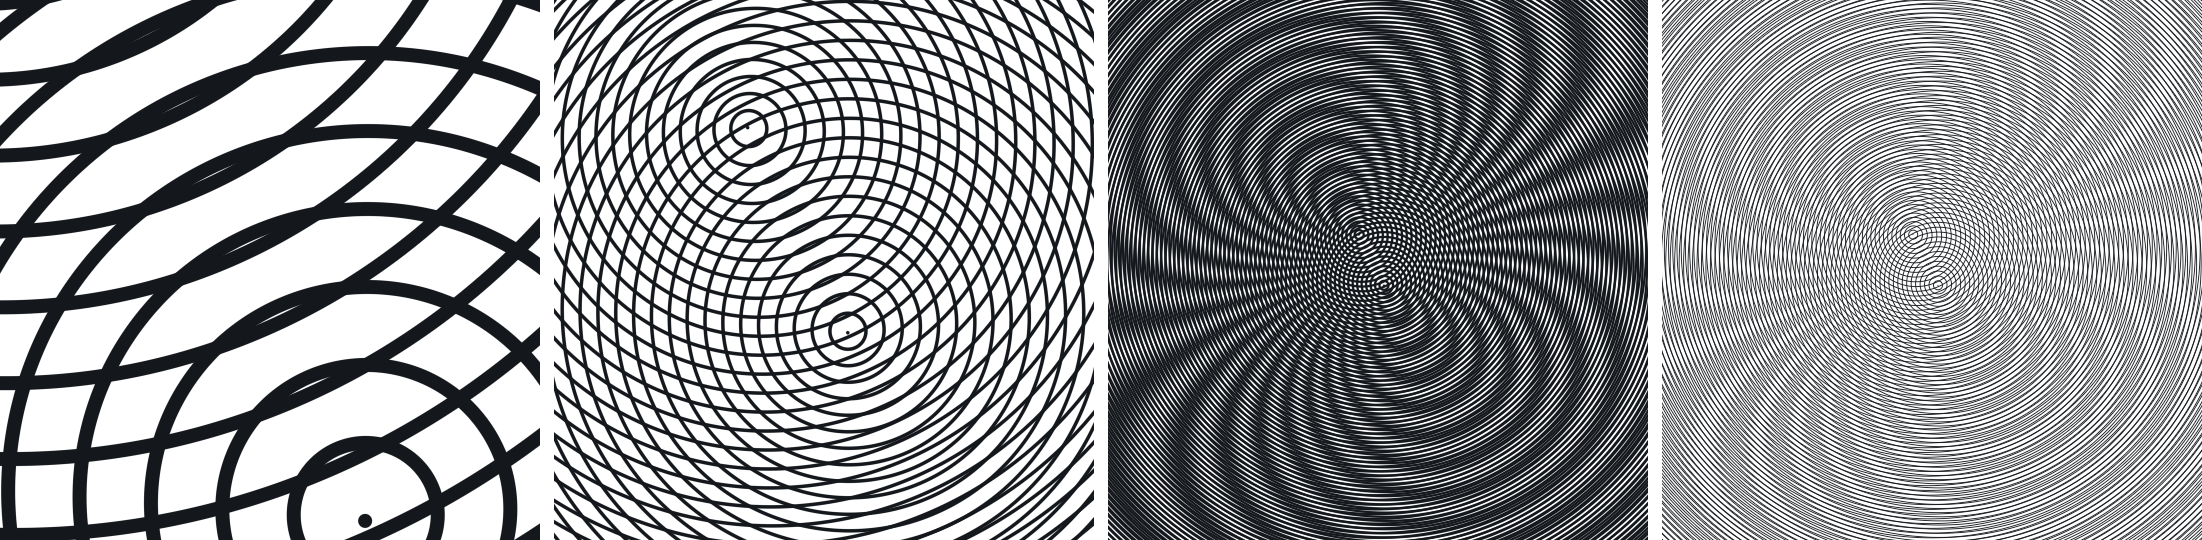
\includegraphics[width=\linewidth]{figures/zoom.png}
  \panelrow{0.24523}{0.00636}{%
    (a) zoom $2$,
    (b) zoom $1$,
    (c) zoom $0.25$,
    {(d) zoom $0.25$, no floor}}
  \Description{Four square panels of the same black-on-white scene at falling zoom.
  The first shows a bold open weave of ring arcs from two centers on the frame's
  diagonal; the second shows the whole two-center rosette, its rings crossing in a
  lens pattern; the third packs the same rosette into a dense dark pinwheel of spiral
  fringe arms; the fourth is the third panel again but washed out to pale gray and
  visibly speckled, with the fringe arms no longer readable.}
  \caption{\figlead{One scene over an eightfold zoom range, with and without
  the stroke floor.}
  Two walking circle families---the tool's default preset, recomposed with its
  centers on the frame's diagonal.
  \textbf{(a--c)}~zoom $2$,
  $1$ and $0.25$. Nothing is resampled between them: each is the same pair of scalar
  fields evaluated on its own grid, so there is no mip level to choose, no filter
  kernel to widen, and no resolution at which the pattern was ever committed. Stroke
  thickness is a \emph{world} quantity and is the same number in all four panels,
  which is why the strokes get thinner on screen as the zoom falls. \textbf{(d)}~the
  same frame as (c) with the stroke floor of \eqref{eq:stroke} removed. All four are
  rendered at one sample per pixel, exactly as the shader does, so (c) and (d) differ
  in one constant and nothing else. The floor is what keeps the fringe system in (c);
  without it the sub-pixel strokes are hit or missed and the pattern goes pale and
  grainy. The floor's cost, the ink it adds, is measured in
  \S\ref{sec:zoom}. (The table there uses a plainer pair, a spiral over rings, since
  the third rule under test needs a family with a closed-form phase.)}
  \label{fig:zoom}
\end{figure*}

\subsection{Continuous transitions between families}

Switching a layer from circles to hexagons is a change of $\ph$, and the direct
implementation of that is a jump. Authors read a jump as breakage, and more
importantly they cannot see \emph{what} changed, which is precisely the thing a
tool for studying interference should show.

So the slot carries two family codes and a mix parameter: the shader evaluates the
distance under both the old family and the new one and interpolates the
\emph{distances}, easing the mix over $280$\,ms with a cubic. Interpolating
distances rather than images means there is one stroke at all times, travelling
from one geometry to the other, instead of two strokes cross-fading. The store snaps to the
target immediately, so the eased value lives only in the uniform and no
undo, export or reload can catch a half-morphed state. Switching to a family for
which the per-member motion is meaningless---lines, lattices, curves---also
zeroes the two walking parameters, because leaving them set produces a layer whose
sliders visibly do nothing.

\subsection{Direct manipulation of a field}

Dragging moves the selected layer in screen space, which requires inverting the
layer's own rotation onto the drag delta or the layer walks away from the cursor;
holding \textsc{alt} rotates the layer about the world origin, the operation that
makes a walking family unwind. The wheel zooms to the cursor, and the first paint
waits on \texttt{compileAsync}, easing two default concentric layers into the
loaded preset with the same morph machinery, so the first thing an author sees is
the mechanism moving into place. Everything else is deliberately thin: one collapsible panel, the envelope and
ratio views of \S\ref{sec:envelope}--\S\ref{sec:visibility} as header
toggles, a still and clip export, and a JSON scene file that saves the
construction---layers, camera, background, and what moves
(\S\ref{sec:time})---and nothing else. A looping parameter is written into that
file at the value its cycle departs from rather than wherever the clock had
carried it, since the instant a file happened to be saved at is a fact about the
session and not about the pattern. There are no layer effects and no inspector;
the pattern is the document.

\subsection{A frame is a function of the clock}
\label{sec:time}

Nothing in the renderer accumulates. There is no history buffer, no progressive
refinement, no temporal filter and no cached raster: a frame is determined by
the twelve slots' uniforms and the handful of camera and view uniforms beside
them, and by nothing else. The animation model is built to keep it that way. An animated parameter is
a function $v(t)$ evaluated afresh every frame rather than a value advanced by
$v \leftarrow v+\dot v\,\Delta t$, and several parameters may share one
\emph{timing}---a delay, a period, a mode and an easing---so that a dozen knobs
move as one gesture instead of as a dozen that drift apart. Parameters that are
functions of the clock, over a renderer that holds no state, make the frame
itself a function of the clock.

Two things follow that a renderer carrying state does not get. Scrubbing is
exact: the frame at $t$ is computed rather than replayed, so seeking backwards
costs what seeking forwards costs and neither depends on where the clock has
been. And capture need not run in real time. The recorder is the clock rather
than an observer of it---it asks for frame $n$ at exactly $t_0+n/\mathrm{fps}$,
renders once synchronously at a stated size, waits for the pixels however long
they take, and only then advances---so a file at $2160$p and $120$\,fps comes
out of a renderer that never has to reach that rate, and the same range recorded
twice is the same file twice. The clip's length is not guessed either: every
animator states its own period, and the tool offers the least common multiple of
them, which is the shortest range at which every cycle has closed and the clip
therefore repeats without a join.

\section{Results}
\label{sec:results}

\subsection{Protocol}
\label{sec:protocol}

We compare four solvers. \sweep{} is the fixed-budget enumeration our renderer
shipped before this work: seed at $\rad(p)/s$, sweep a constant number of
neighbours, refine with Newton. \loose{} is the interval of
Theorem~\ref{thm:window} with the drift constant~\eqref{eq:drift} replaced by
$\lVert\delta\rVert$, isolating the contribution of
Section~\ref{sec:drift}. \ours{} is the full method. \textsc{Reference} is an
exhaustive scan at stride $1$ with no budget and no interval, terminating only on
the trivial certificate $\rad(q_n)\le \lVert p\rVert + nm$; it is independent of
the bound under test, so it can referee it.

The GPU numbers come from a standalone WebGPU harness that extracts the WGSL of
each solver generation directly from its source file, compiles it into an
identical compute kernel, and times a pass with GPU timestamp queries over a
$1200\times800$ point grid --- $0.96$\,Mpixel of solver work with no
rasterisation, no compositing, and no browser frame overhead in the measurement.
Reported values are the median of $9$ passes after $3$ warm-up passes, on an
Apple \texttt{\gpuAdapter} adapter. The CPU numbers come from a rasteriser that
mirrors the shader's compositing term for term, instrumented to count calls to
$\rad$; this is the only way to render an image with a solver that no longer
exists in the shader, and the only way to get a per-pixel work map.

All experiment scripts, the generated data, and every figure in this paper are in
the accompanying repository and reproduce with one command each.

\subsection{Cost}

% GENERATED by paper/tools/numbers.mjs
\begin{table}[t]
  \centering
  \small
  \caption{GPU pass time in milliseconds per megapixel of solver work, one
  full-screen family, Apple \texttt{metal-3}. \emph{Zoom} $0.15$ is a $6.7\times$
  zoom-out, where the index interval is widest. The last three rows are the hard
  cases of Section~\ref{sec:limits}: an offset close to the spacing, and the
  marginal drift $m=s$ itself. Bold marks the shipped method, not the row minimum:
  \loose{} is faster on the nonagon row, and loses ink globally
  (Table~\ref{tab:fidelity}).}
  \label{tab:gpu}
  \begin{tabular}{llrrr}
    \toprule
    Family & Zoom & \sweep{} & \loose{} & \ours{} \\
    \midrule
    Circle, rotation + offset & $1$ & $10.16$ & $0.33$ & $\mathbf{0.33}$ \\
    Circle, rotation + offset & $0.15$ & $15.47$ & $1.25$ & $\mathbf{1.05}$ \\
    Square, rotation & $1$ & $8.78$ & $0.26$ & $\mathbf{0.26}$ \\
    Square, rotation + offset & $0.15$ & $13.50$ & $0.85$ & $\mathbf{0.79}$ \\
    Square, offset only & $1$ & $0.92$ & $1.18$ & $\mathbf{0.20}$ \\
    Triangle, rotation & $1$ & $14.42$ & $0.52$ & $\mathbf{0.39}$ \\
    Triangle, rotation & $0.15$ & $20.12$ & $1.44$ & $\mathbf{0.92}$ \\
    Triangle, rotation + offset & $1$ & $16.97$ & $0.79$ & $\mathbf{0.52}$ \\
    Triangle, rotation + offset & $0.15$ & $27.85$ & $2.69$ & $\mathbf{1.64}$ \\
    Hexagon, rotation + offset & $0.15$ & $25.17$ & $2.23$ & $\mathbf{1.64}$ \\
    Nonagon, rotation + offset & $0.15$ & $23.40$ & $2.03$ & $\mathbf{2.16}$ \\
    \midrule
    Offset near spacing & $1$ & $43.32$ & $2.82$ & $\mathbf{1.57}$ \\
    Offset near spacing & $0.15$ & $46.73$ & $7.47$ & $\mathbf{5.44}$ \\
    Marginal drift $m=s$ & $1$ & $65.73$ & $30.47$ & $\mathbf{17.56}$ \\
    \bottomrule
  \end{tabular}
\end{table}

% GENERATED by paper/tools/numbers.mjs
\begin{table}[t]
  \centering
  \small
  \caption{Mean evaluations of $\rad$ per pixel, CPU rasterizer, and fraction of
  pixels differing from \textsc{Reference} by more than $8/255$. \ours{} agrees
  with brute force to within that tolerance at every pixel of all 7 scenes
  while doing less work than the exhaustive scan that defines the reference.}
  \label{tab:cost}
  \begin{tabular}{@{}lrrrr@{}}
    \toprule
    & \multicolumn{3}{c}{evaluations / pixel} & \ours{} \\
    \cmidrule(lr){2-4}
    Scene & \textsc{Ref.} & \sweep{} & \ours{} & differ \\
    \midrule
    Triangle, rotation & $21.9$ & $192.3$ & $7.6$ & $0.0\%$ \\
    Hexagon, rotation, zoomed out & $84.3$ & $180.0$ & $9.0$ & $0.0\%$ \\
    Triangle, translation & $19.2$ & $195.4$ & $11.0$ & $0.0\%$ \\
    Triangle, offset $=$ spacing & $46.0$ & $283.6$ & $11.0$ & $0.0\%$ \\
    Square, rotation + translation & $23.5$ & $201.9$ & $7.8$ & $0.0\%$ \\
    Deep zoom-out, small rotation & $43.5$ & $194.1$ & $\mathbf{7.5}$ & $0.0\%$ \\
    Two circle families, interfering & $49.5$ & $360.8$ & $11.1$ & $0.0\%$ \\
    \bottomrule
  \end{tabular}
\end{table}


Table~\ref{tab:gpu} gives GPU pass times. Across rotated settings \ours{} is
$\gpuSpeedLo$--$\gpuSpeedHi\times$ faster than \sweep{}. The absolute numbers are
what changed the tool: a single rotated triangle family went from
$\gpuTriRotOne$\,ms per megapixel --- alone, over budget for a $60$\,Hz frame ---
to $\gpuTriRotOneNew$\,ms, so a dozen layers now fit in the frame that one layer
used to miss. At $6.7\times$ zoom-out, where \sweep{} degrades to
$\gpuTriRotOffOut$\,ms, \ours{} costs $\gpuTriRotOffOutNew$\,ms. The
translation-only row shows Proposition~\ref{prop:closed} in isolation:
$\gpuSquareOld \to \gpuSquareClosed$\,ms, a $\gpuSquareClosedGain\times$ gain over
an already-cheap case, because the closed form needs no rotation and hence no
transcendentals.

Table~\ref{tab:cost} counts CPU evaluations of $\rad$ per pixel and, in the last
column, disagreement with the exhaustive reference. Two things stand out. \ours{}
costs $\costOursLo$--$\costOursHi$ evaluations per pixel where \sweep{} costs
$\costSweepLo$--$\costSweepHi$ --- a $\costVsSweepLo$--$\costVsSweepHi\times$
reduction in the quantity the shader actually pays for. And \ours{} is cheaper than
\textsc{Reference} itself, by $\costVsRefLo$--$\costVsRefHi\times$, despite
\textsc{Reference} being given a termination
certificate: the Lipschitz rule skips indices the exhaustive scan is obliged to
visit. Being faster than brute force while agreeing with it everywhere is the
cleanest summary of the method we can offer.

\subsection{Fidelity}

\begin{figure*}[t]
  \centering
  \begin{subfigure}{0.245\textwidth}
    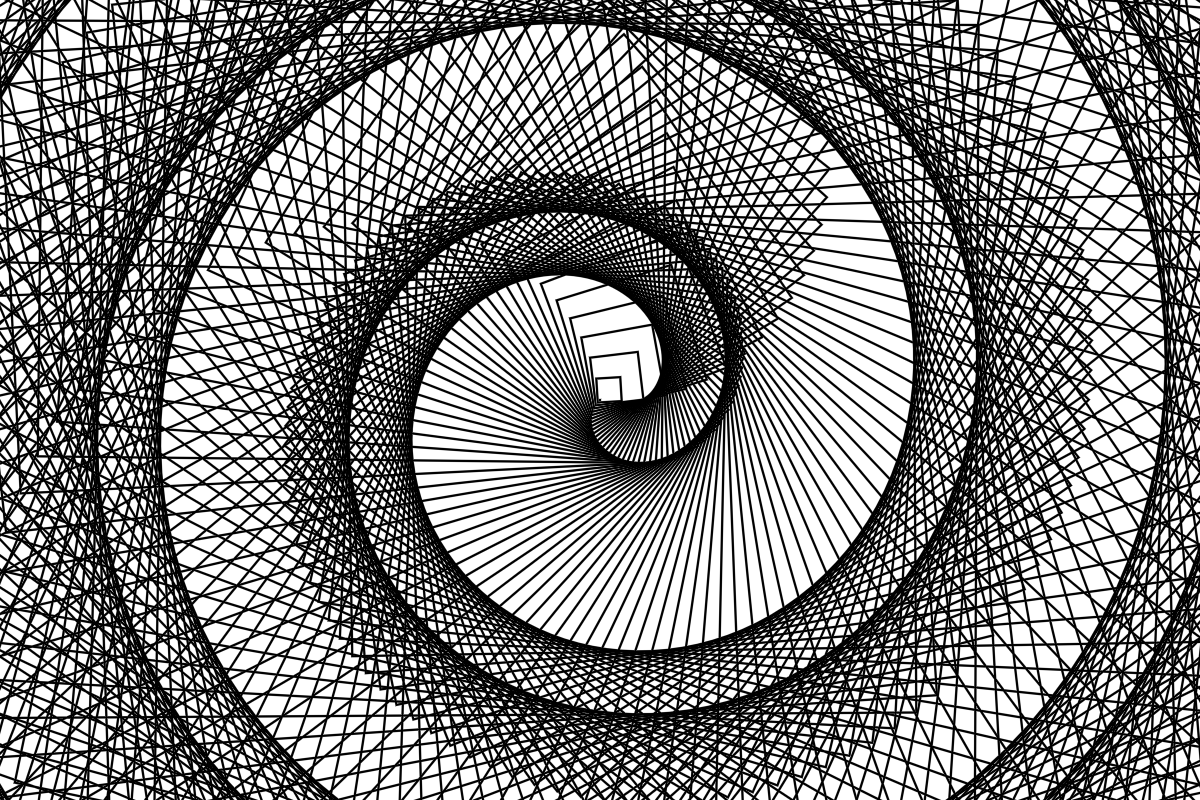
\includegraphics[width=\linewidth]{figures/artifact-holes-reference.png}
    \caption{\textsc{Reference}}
  \end{subfigure}\hfill
  \begin{subfigure}{0.245\textwidth}
    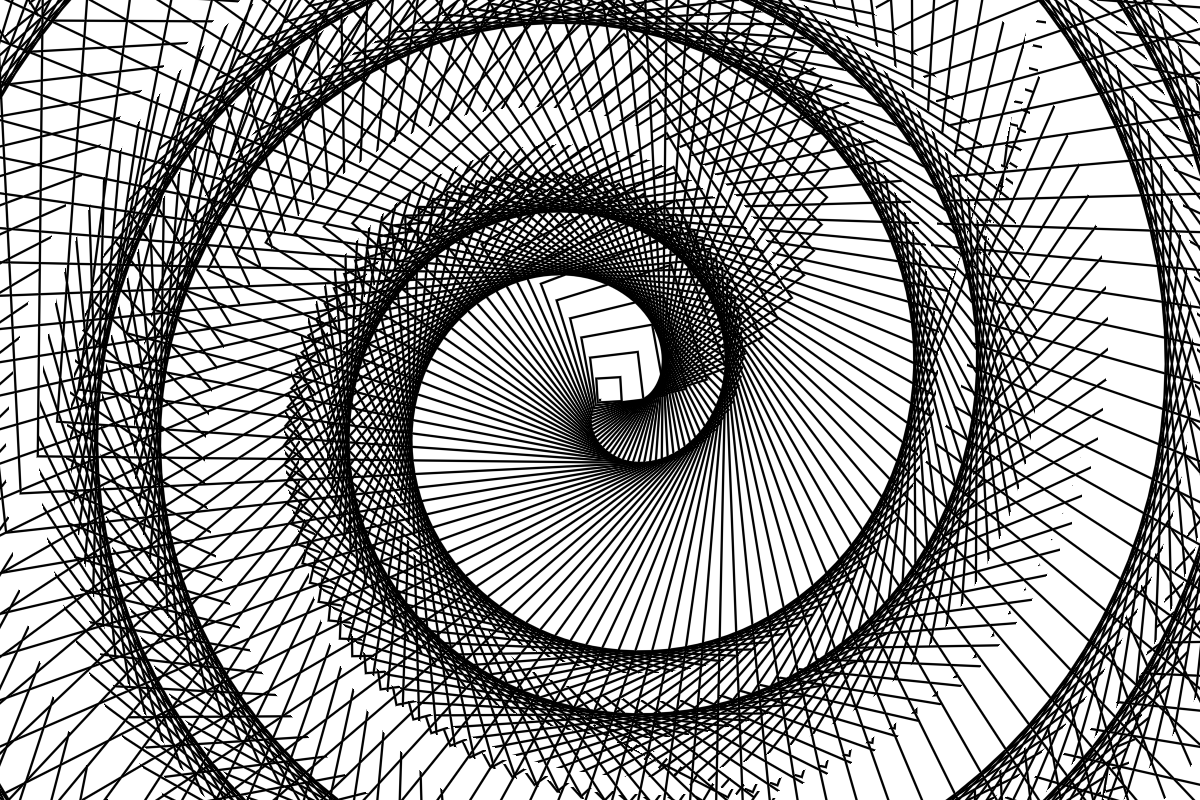
\includegraphics[width=\linewidth]{figures/artifact-holes-sweep.png}
    \caption{\sweep{}, $\artHolesSweepEv$ ev/px}
  \end{subfigure}\hfill
  \begin{subfigure}{0.245\textwidth}
    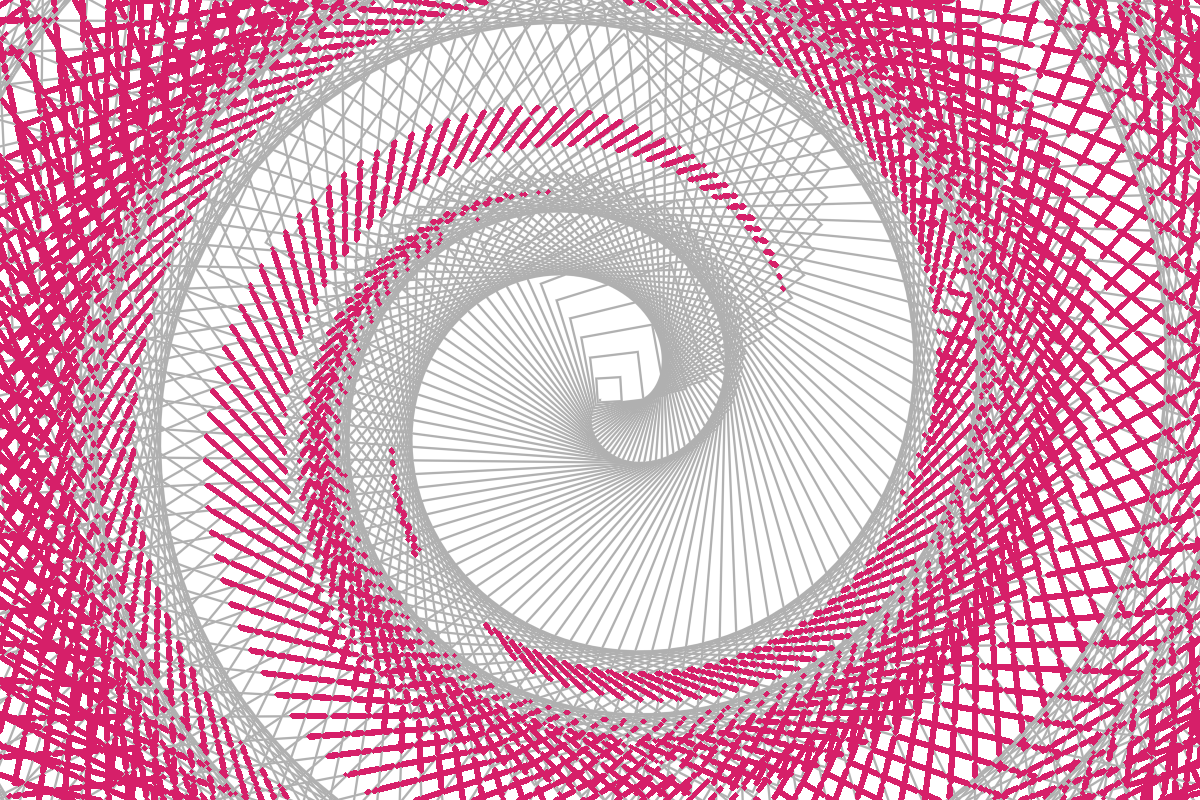
\includegraphics[width=\linewidth]{figures/artifact-holes-sweep-drop.png}
    \caption{lost ink (magenta)}
  \end{subfigure}\hfill
  \begin{subfigure}{0.245\textwidth}
    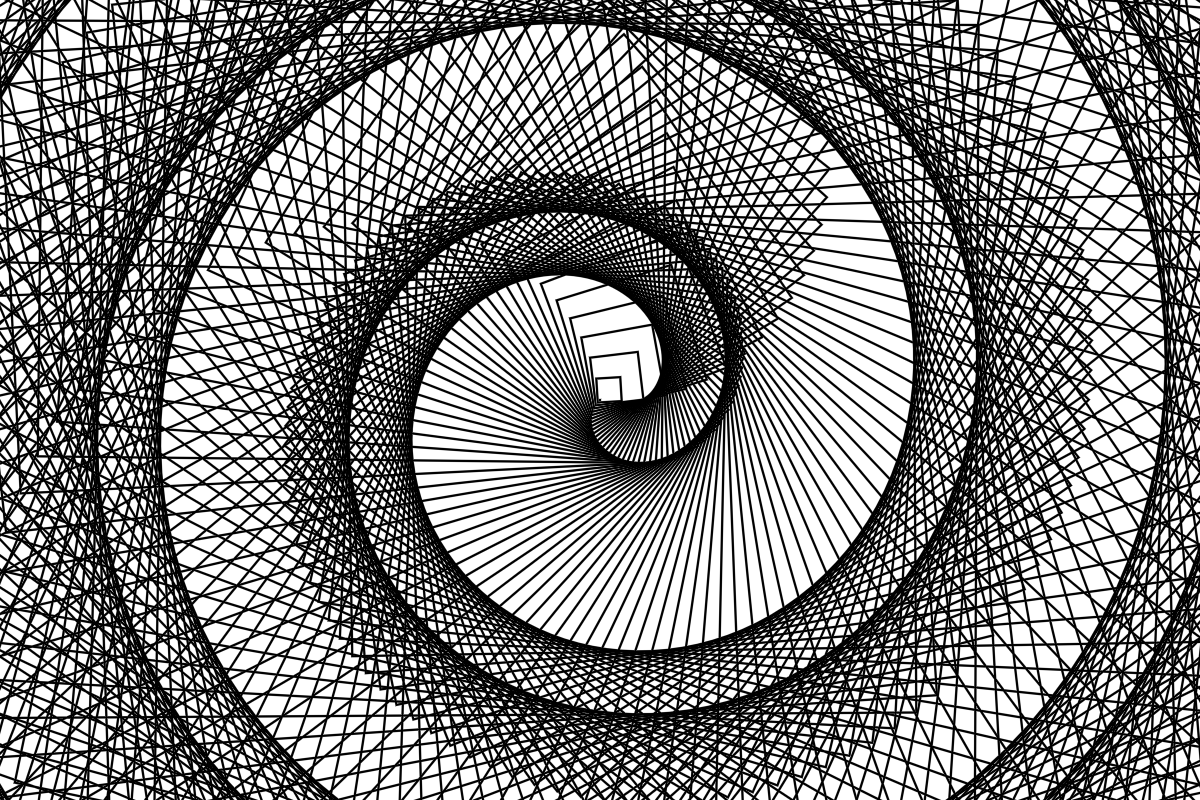
\includegraphics[width=\linewidth]{figures/artifact-holes-final.png}
    \caption{\ours{}, $\artHolesOursEv$ ev/px}
  \end{subfigure}
  \Description{Four wide panels of the same black-on-white field of walking
  hexagons, seen far from the family's centre: layers of finely woven arcs
  sweeping across the frame like drapery, with smooth dark bands between them.
  The first and fourth are identical. The second is visibly paler, with whole
  bands of the weave missing. The third is a pale grey copy of the pattern in
  which only the lost segments are drawn, in magenta, showing that the losses
  form broad coherent ribbons that follow the bands rather than scattered
  pixels.}
  \caption{Fixed enumeration deletes arcs, not pixels. The far field of a
  walking hexagon family whose drift aims at an edge --- almost a full spacing
  long, $\lVert\delta\rVert=0.95s$, while the support ratio stays at
  $\rad(-\delta)/s=0.82$; \sweep{} loses $\artHolesSweepDiff\%$ of the frame's
  pixels, and because the failure condition varies smoothly with $p$ the losses
  organise into coherent ribbons that read as missing bands. \ours{} is
  pixel-identical to the reference using $\artHolesSaving\times$ less work than
  \sweep{}. Insets in Figure~\ref{fig:insets}.}
  \label{fig:holes}
\end{figure*}

\begin{figure}[t]
  \centering
  \begin{subfigure}{0.32\linewidth}
    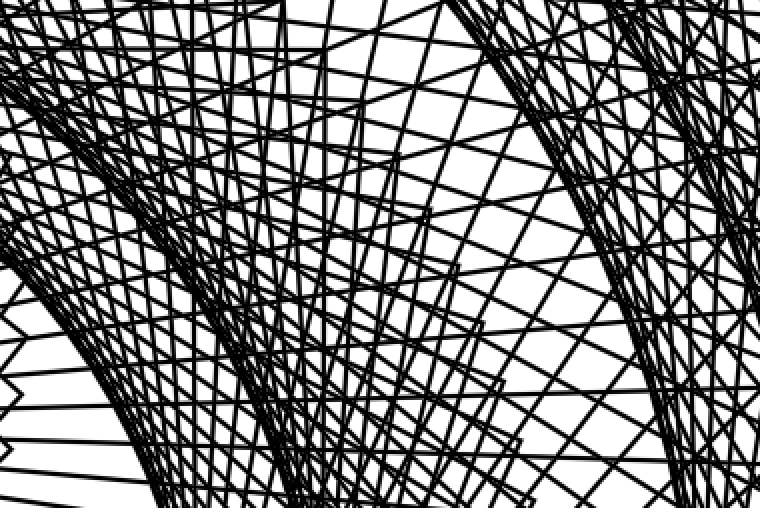
\includegraphics[width=\linewidth]{figures/inset-holes-reference.png}
    \caption{\textsc{Reference}}
  \end{subfigure}\hfill
  \begin{subfigure}{0.32\linewidth}
    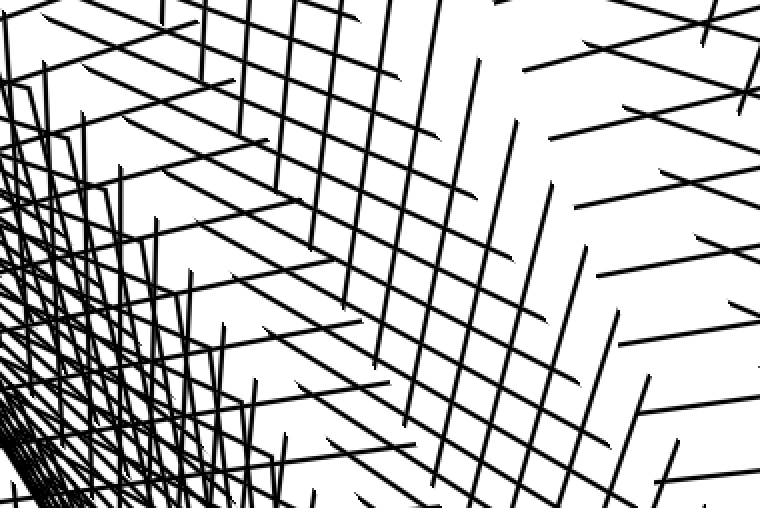
\includegraphics[width=\linewidth]{figures/inset-holes-sweep.png}
    \caption{\sweep{}}
  \end{subfigure}\hfill
  \begin{subfigure}{0.32\linewidth}
    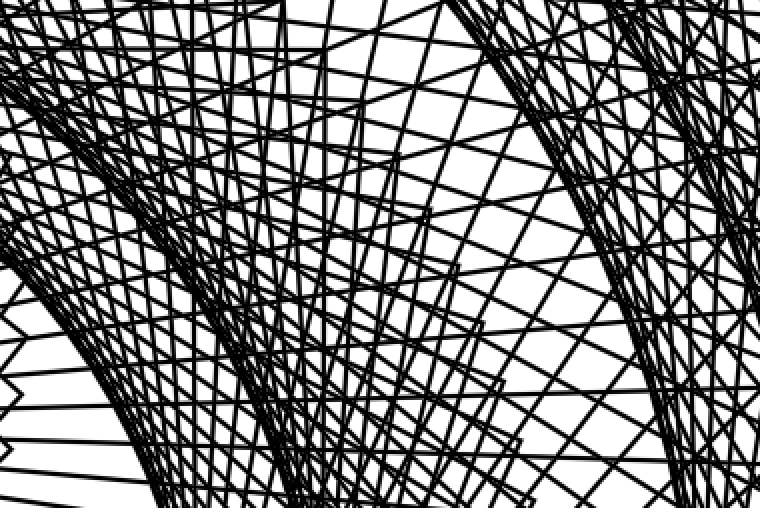
\includegraphics[width=\linewidth]{figures/inset-holes-final.png}
    \caption{\ours{}}
  \end{subfigure}
  \Description{Three magnified crops of a hatched pattern of crossing arcs. The
  first and third are identical and continuous. In the second, several arcs stop
  part-way across the crop and resume further on, leaving clean gaps.}
  \caption{$2\times$ crop of the worst region of Figure~\ref{fig:holes}. The
  missing ink is not noise; it is whole segments of whole rings, which is why the
  artifact survives supersampling and reads as a modelling error rather than an
  aliasing one.}
  \label{fig:insets}
\end{figure}

\begin{figure}[t]
  \centering
  \begin{subfigure}{0.32\linewidth}
    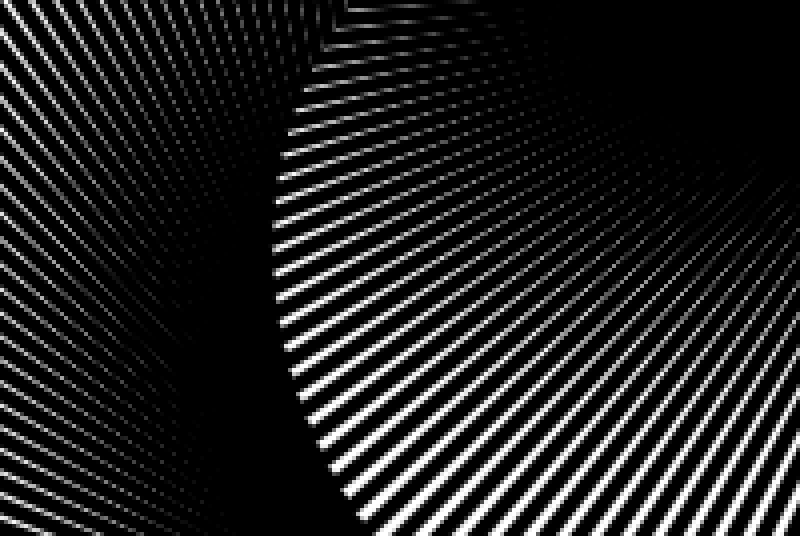
\includegraphics[width=\linewidth]{figures/inset-drift-reference.png}
    \caption{\textsc{Reference}}
  \end{subfigure}\hfill
  \begin{subfigure}{0.32\linewidth}
    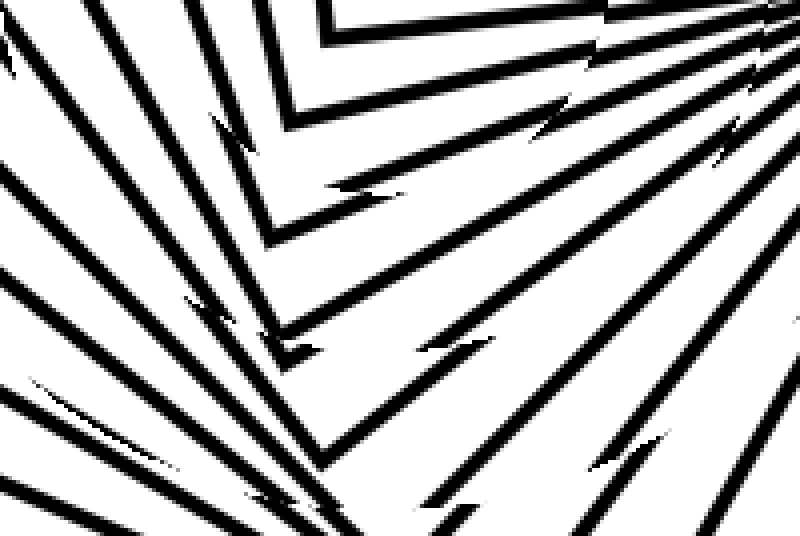
\includegraphics[width=\linewidth]{figures/inset-drift-window1.png}
    \caption{\loose{}}
  \end{subfigure}\hfill
  \begin{subfigure}{0.32\linewidth}
    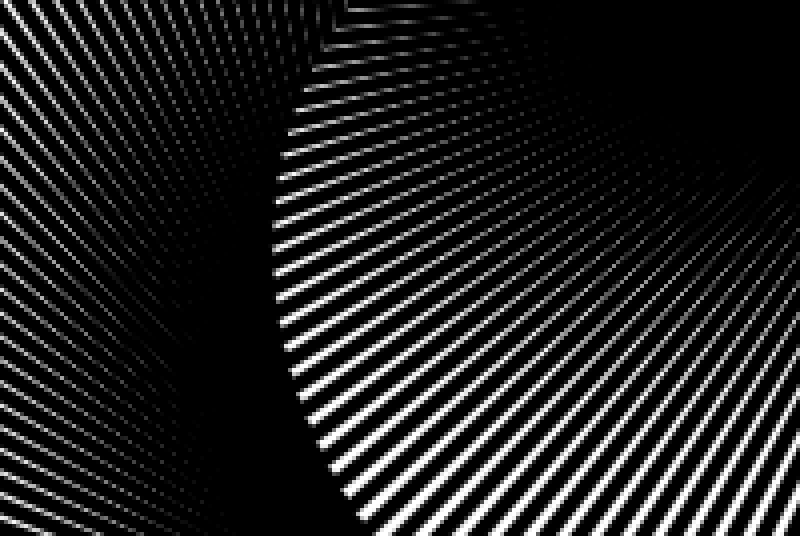
\includegraphics[width=\linewidth]{figures/inset-drift-final.png}
    \caption{\ours{}}
  \end{subfigure}
  \Description{Three magnified crops of a fan of straight strokes on black. The
  first and third match. The second has lost roughly two thirds of the strokes
  uniformly, so it reads as a sparser fan rather than a damaged one.}
  \caption{A loose drift constant is worse than a slow solver. \loose{} differs
  from~\eqref{eq:drift} only by using $\lVert\delta\rVert$ in place of
  $\rad(-\delta)$. That is enough to declare this setting's interval too wide to
  scan, so it subsamples: ink drops from $\artDriftRefInk$ to
  $\artDriftLooseInk$ and $\artDriftLooseDiff\%$ of pixels change. The exact
  constant keeps the interval finite and the pattern intact.}
  \label{fig:drift}
\end{figure}

We swept $\fidSettings$ parameter settings --- six shapes $\times$ spacings from
$1$ to $120$ $\times$ offsets $\times$ rotations $\times$ six zoom levels ---
and compared every solver against \textsc{Reference} at $512$ quasi-random points
each, classifying each point as agreeing, having lost ink, or having invented it.
Settings where the exhaustive reference would need more than $10^5$ evaluations
per point are counted and excluded rather than measured. Results in
Table~\ref{tab:fidelity}.

\begin{table}[t]
  \centering
  \small
  \caption{Ink lost against \textsc{Reference} over $\fidSettings$ settings.
  \emph{In interval} restricts to points where Theorem~\ref{thm:window}'s interval
  fits the budget, so exactness is claimed; \emph{legible} restricts to the
  $\fidLegible$ settings whose exact field is under $70\%$ ink, i.e. where a
  pattern is still visible. No solver ever invented ink, since all three minimise
  over a subset of $\N_0$.}
  \label{tab:fidelity}
  \begin{tabular}{lccc}
    \toprule
    & \sweep{} & \loose{} & \ours{} \\
    \midrule
    settings with holes            & $\fidSweepHoles$ & $\fidLooseHoles$ & $\fidOursHoles$ \\
    worst ink lost                 & $\fidSweepWorst\%$ & $\fidLooseWorst\%$ & $\fidOursWorst\%$ \\
    \midrule
    \emph{in interval}: settings   & $\fidSweepEnvelopeHoles$ & $\fidLooseEnvelopeHoles$ & $\mathbf{0}$ \\
    \emph{in interval}: worst      & $\fidSweepEnvelopeWorst\%$ & $\fidLooseWorst\%$ & $\mathbf{0.0\%}$ \\
    \midrule
    \emph{legible}: settings       & $\fidSweepLegibleHoles$ & $0$ & $\mathbf{0}$ \\
    \emph{legible}: worst          & $\fidSweepLegibleWorst\%$ & $0.0\%$ & $\mathbf{0.0\%}$ \\
    \bottomrule
  \end{tabular}
\end{table}

The row that matters is the third block. Wherever the proven interval fits the
budget --- the regime in which Theorem~\ref{thm:window} claims exactness --- \ours{}
disagrees with brute force at zero points out of $\fidSettings$ settings, while
\sweep{} disagrees in $\fidSweepEnvelopeHoles$ settings and loses up to
$\fidSweepEnvelopeWorst\%$ of the ink, and \loose{} up to $\fidLooseWorst\%$. The
theorem is not doing bookkeeping; it is the difference between an image and a
damaged one.

The $\fidOursHoles$ settings where \ours{} does lose ink are all outside the
envelope, and all of them are saturated: every one has an exact ink fraction above
$70\%$. Across the $\fidLegible$ legible settings, \ours{} loses nothing anywhere.
That is the honest form of the claim: exact where it claims to be, and in
particular exact everywhere a user can see a pattern.

Figures~\ref{fig:holes} and~\ref{fig:insets} show what the \sweep{} column looks
like on one scene, and Figure~\ref{fig:drift} isolates the drift constant. The
GPU twin agrees with the CPU twin to \texttt{f32} precision at every point where
the interval fits the budget.

\subsection{Ablation}

% GENERATED by paper/tools/numbers.mjs
\begin{table}[t]
  \centering
  \small
  \caption{Time relative to the full method when one mechanism is removed
  ($3.84$\,Mpixel of solver work). Each column is a different family, chosen so
  that every mechanism has a column where it binds. Values below $1$ mean the
  mechanism costs time in that setting, which is the price of exactness
  elsewhere.}
  \label{tab:ablation}
  \begin{tabular}{lcccc}
    \toprule
     & \multicolumn{2}{c}{rotated} & \multicolumn{2}{c}{translated} \\
    \cmidrule(lr){2-3}\cmidrule(lr){4-5}
    Mechanism removed & tri. & hex.\ out & near $s$ & marginal \\
    \midrule
    Lipschitz skip (\S\ref{sec:skip}) & $2.03$ & $2.29$ & $3.12$ & $1.00$ \\
    Support fast paths (\S\ref{sec:walking}) & $1.31$ & $1.16$ & $1.00$ & $1.49$ \\
    Exact drift (\S\ref{sec:drift}) & $1.00$ & $1.00$ & $1.25$ & $1.00$ \\
    Polygon closed form (\S\ref{sec:closed}) & $0.97$ & $0.99$ & $0.98$ & $\mathbf{101.2}$ \\
    Carried rotation (\S\ref{sec:skip}) & $0.95$ & $0.91$ & $0.93$ & $1.01$ \\
    Accept early exit (\S\ref{sec:guard}) & $0.91$ & $0.91$ & $0.90$ & $1.04$ \\
    \bottomrule
  \end{tabular}
\end{table}


Table~\ref{tab:ablation} removes one mechanism at a time. The Lipschitz skip is
the largest single lever ($\ablSkipLo$--$\ablSkipHi\times$), and the polygon closed
form is decisive exactly where predicted: on the marginal drift it is worth
$\ablClosedMarginal\times$, because without it the scan must walk a $2^{16}$-wide
interval to find an answer that Proposition~\ref{prop:closed} reads off in one
comparison.

Two entries are below $1$: removing the carried rotation or the accept-early-exit
is $\ablCostLo$--$\ablCostHi\%$ \emph{faster} in these dense scenes, a wavefront-%
divergence effect. We keep both because they are what make sparse and mid-density
scenes cheap; the divergence reading, and why narrowing the interval rather than
exiting sooner is the productive lever on a GPU, are in the supplemental
material (\S S3).

\subsection{Where the guarantee ends}
\label{sec:limits}

\begin{figure}[t]
  \centering
  \begin{tikzpicture}
    \begin{axis}[paperaxis, height=5.6cm,
      xlabel={interval span (indices, $\log_2$ bins)},
      ylabel={exact ink fraction},
      xmode=log, log basis x=2,
      xmin=1.5, xmax=131072, ymin=0, ymax=1,
      legend style={at={(0.5,-0.44)}, anchor=north, draw=none, fill=none,
                    /tikz/every even column/.append style={column sep=0.5cm}},
      legend columns=3,
    ]
      \addplot[draw=none, fill=cool!12, forget plot] coordinates
        {(1024,0) (131072,0) (131072,1) (1024,1)} \closedcycle;
      \addplot[cool, very thick, mark=*, mark size=1.3pt]
        table [x=span, y=medianInk, col sep=comma] {data/saturation.csv};
      \addlegendentry{median}
      \addplot[warm, thick, mark=square*, mark size=1.1pt]
        table [x=span, y=q25, col sep=comma] {data/saturation.csv};
      \addlegendentry{lower quartile}
      \addplot[accent, thick, densely dashed]
        table [x=span, y=minInk, col sep=comma] {data/saturation.csv};
      \addlegendentry{minimum}
      \node[soft, font=\scriptsize, anchor=south east] at (rel axis cs: 0.995, 1.015)
        {beyond budget $B$};
      \node[anchor=north west, inner sep=1.5pt, fill=white, draw=soft, semithick]
        at (rel axis cs: 0.035, 0.95) {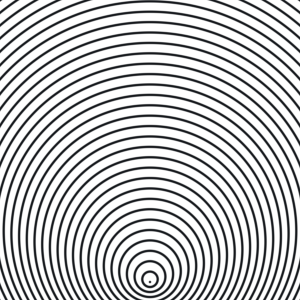
\includegraphics[width=1.35cm]{figures/inset-saturation-open.png}};
      \node[anchor=south east, inner sep=1.5pt, fill=white, draw=soft, semithick]
        at (rel axis cs: 0.90, 0.26) {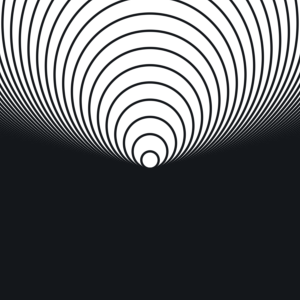
\includegraphics[width=1.35cm]{figures/inset-saturation-solid.png}};
    \end{axis}
  \end{tikzpicture}
  \Description{A line plot of exact ink fraction against interval span on a base-two
  logarithmic axis. Median and lower-quartile curves both rise monotonically from
  near zero at span two to about $0.9$ by span $2^{10}$, where a shaded region marks
  the budget and beyond which both stay high. A dashed minimum curve stays near zero
  until roughly span $2^{10}$ and then rises only to about $0.2$.}
  \caption{The interval is wide only where the pattern is already solid.
  $\satSettings$ settings, binned by the $90$th-percentile interval span, against
  the ink fraction of the exact field. Past the budget $B=\satBudget$ (shaded) the median
  setting is $\satMedianInk$ ink --- a nearly filled rectangle, where no point
  sample of the distance field is meaningful and the honest output is the filtered
  mean~\cite{Norton1982}. The insets are one walking circle family at both ends
  of the axis: a benign drift, whose pattern is open and whose interval is a few
  indices, and the near-marginal drift, where the interval explodes --- into a
  frame that is already solid ink. The dashed minimum is the honest caveat: sparse
  exceptions exist.}
  \label{fig:saturation}
\end{figure}

\begin{figure}[t]
  \centering
  \begin{subfigure}{0.32\linewidth}
    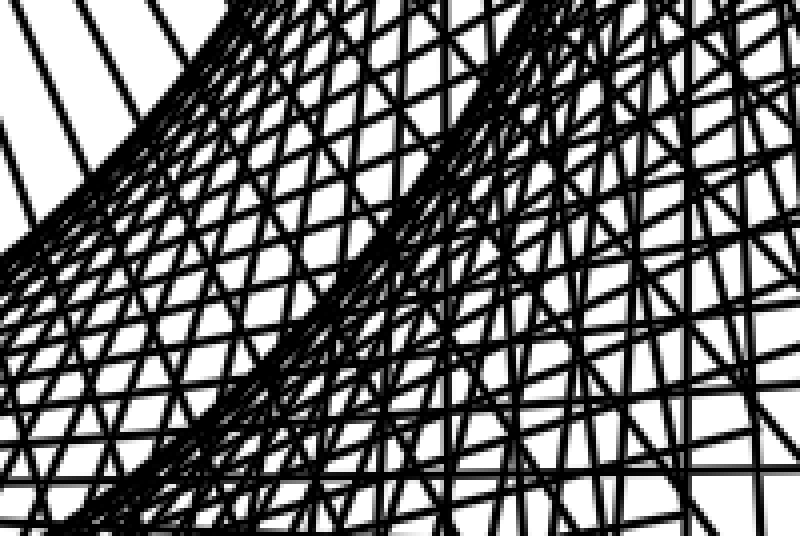
\includegraphics[width=\linewidth]{figures/inset-anchor-reference.png}
    \caption{exact}
  \end{subfigure}\hfill
  \begin{subfigure}{0.32\linewidth}
    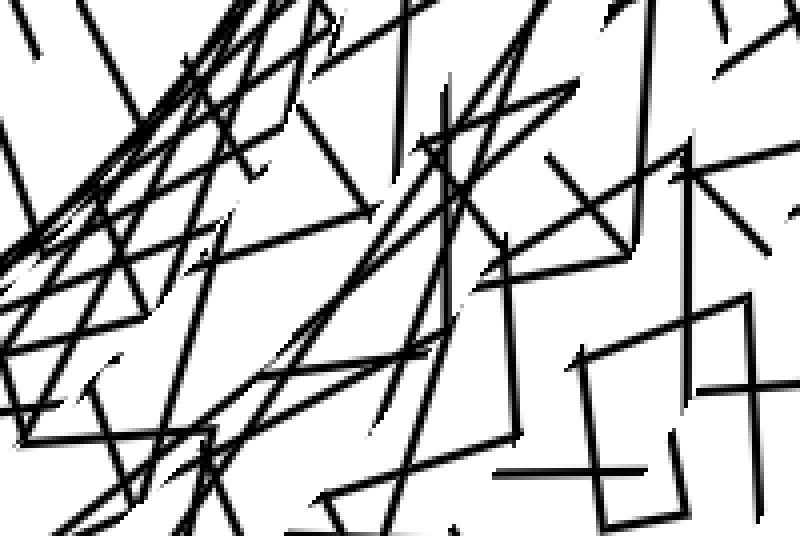
\includegraphics[width=\linewidth]{figures/inset-anchor-pixel-anchored.png}
    \caption{pixel-anchored}
  \end{subfigure}\hfill
  \begin{subfigure}{0.32\linewidth}
    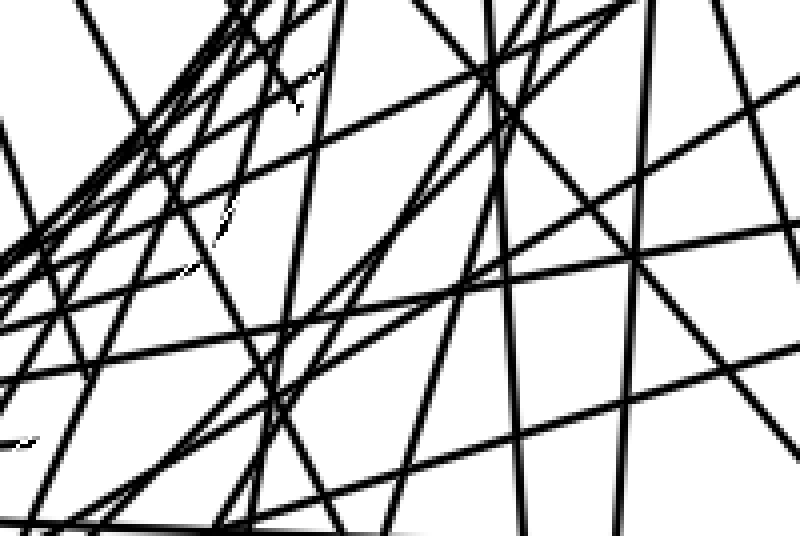
\includegraphics[width=\linewidth]{figures/inset-anchor-lattice-anchored.png}
    \caption{lattice-anchored}
  \end{subfigure}
  \Description{Three heavily magnified crops of a crosshatch of straight strokes.
  The first is a clean lattice of crossings. The second has broken into short
  disconnected dashes and hooks with no continuous line anywhere. The third is a
  clean lattice again, sparser than the first but with every stroke whole.}
  \caption{When you cannot be exact, be coherent. $4\times$ crops of one scene
  with the budget forced to $64$ so the stride engages while the field is still
  legible. Both subsamplings spend $\artAnchorEv$ evaluations per pixel and retain
  the same ink ($\artAnchorPixelInk$ vs $\artAnchorLatticeInk$ of the exact
  $\artAnchorRefInk$). Anchoring the stride to the pixel's own interval (centre) makes
  neighbouring pixels sample different rings, and the pattern shatters into dashes
  and hooks. Anchoring it to the global index lattice (right) makes them agree, and
  the same missing ink becomes a thinner family of whole straight lines --- a
  plausible pattern rather than a broken one. The two differ by one line of code.}
  \label{fig:anchor}
\end{figure}

Theorem~\ref{thm:window} gives an interval; it does not promise a small one. Two
questions follow: how often is it too wide to walk, and what happens then.

\emph{How often.} Over $\satSettings$ settings spanning the whole parameter space
our interface exposes, the interval fits the $B=\satBudget$ budget in $\satFitting$ of
them ($\satFittingPct\%$), and the widest fitting span we observed is
$\satWidestFitting$ --- so the budget is nearly exactly the right size, not an
arbitrary large number. In the remaining $\satStrided$ the interval exceeds the
budget. Every one of those has $m$ within a factor of $\satDriftRatioHi$ of $s$;
the wide-interval regime is precisely the near-marginal band, as the theory
predicts.

\emph{What the field looks like there.} Figure~\ref{fig:saturation} answers this
without needing an exhaustive reference, using the observation that any partial
scan takes a minimum over a subset and therefore \emph{over}-estimates $d$ and
\emph{under}-estimates ink: a measured ink fraction is a valid lower bound on the
true one. Ink rises monotonically with interval span, and past the budget the median
setting is $\satMedianInk$ ink. These are fields whose curves are far denser than
the pixel grid --- the regime where point sampling any distance field is
meaningless and the correct answer is a prefiltered
mean~\cite{Norton1982, Bruneton2012}. Only $\satStridedLegible$ settings
($\satStridedLegiblePct\%$ of the sweep) are both beyond the budget and legible.

\emph{What we lose there.} For those we cannot use the exhaustive reference, so we
compare against the same solver with $B$ raised to $131072$, which walks every
index inside the span cap at stride $1$. Over $\degChecked$ strided settings,
$\degWithDrop$ lose some ink; the mean loss is $\degMean\%$ and the worst is
$\degWorst\%$, in a setting whose exact field is $100\%$ ink. Restricted to the
$\degLegible$ legible ones the worst loss is $\degLegibleWorst\%$. We do not
claim correctness here and we do not claim a prefiltered mean; this is a genuine
limitation, confined to a $\satStridedLegiblePct\%$ band of parameter space, and it
is the obvious target for future work (Section~\ref{sec:future}).

\emph{What we do about it.} What we can control is the \emph{structure} of the
error, and Figure~\ref{fig:anchor} is the one finding here we would ask an
implementor to keep.
Both panels subsample by the same stride, spend the same $\artAnchorEv$ evaluations
per pixel, and retain statistically the same ink. Anchoring the stride to
$n_{\mathrm{lo}}$ --- which depends on the pixel --- makes adjacent pixels sample
disjoint subsets of rings, and the pattern disintegrates into dashes. Anchoring it
to multiples of the stride makes every pixel in a neighbourhood agree on which
rings exist, and the same amount of missing ink becomes a thinner family of whole
curves. The error is identical in magnitude and completely different in kind. Since
a viewer reads structure and not coverage, this is the difference between an
approximation and a bug, and it costs nothing.

\section{Fringes as an instrument}
\label{sec:beyond}

Everything so far has treated the index difference $D=\idx_1-\idx_2$ as an
\emph{output}: two families are given, $D$ is whatever they imply, and the fringe
law (Theorem~\ref{thm:fringe}) tells us what we will see. This section runs the
arrow backwards. If the fringes are the unit level sets of $D$, and $D$ is
something we write in a shader, then we may choose the fringes.

\subsection{Encoding a field in the difference}

Let $f:\R^2\to\R$ be any scalar field, and let $a>0$ be a gain. Take a carrier:
any family of phase $\ph_1$ and pitch $s$. Pair it with a second family defined
by
\begin{equation}
  \ph_2(p) \;=\; \ph_1(p) \;-\; a\,s\,f(p).
  \label{eq:encode}
\end{equation}
Both families have the same pitch, so $\idx_i=\ph_i/s$ and
\begin{equation}
  D(p) \;=\; \idx_1(p)-\idx_2(p) \;=\; a\,f(p).
  \label{eq:contourlaw}
\end{equation}
By Theorem~\ref{thm:fringe} the light fringes are $\{D\in\Z\}$, which is
$\{f=n/a\}$: the contours of $f$ at interval $c=1/a$. Not an approximation of
them, and not a discretization of them, but the same curves a contour tracer
would be trying to find. (For a circle-valued $f$ the same construction mints
the quantized defects of \S\ref{sec:defects}.)

Notice everything that does \emph{not} appear. There is no
marching squares, no cell table, no ambiguous saddle, no polyline, no stitching
of segments into curves, no decision about topology, and no resolution at which
any of that would have happened. The contour is never computed. It is a place
where two strokes coincide, and it is drawn by the same distance query and the
same antialiasing the strokes already had.

Because $a$ and $s$ appear only in the product $as$, \eqref{eq:encode} is a
\emph{shift of the phase residual} and nothing else, which is why it costs so
little to ship. \S\ref{sec:catalog} writes every family as $\{\ph=ns+\varphi\}$ and
inks it through $\mathrm{periodicDist}(\ph-\varphi,s)/|\nabla\ph|$; encoding $f$
subtracts $a s f$ inside that residual and subtracts the vector $a s \nabla f$
from the carrier gradient it divides by. Two extra terms, one shared by all
fourteen families (for the concentric and walking families the carrier
direction in that divide is the radial direction from the layer origin, a
first-order convenience).

The gradient term is not optional. Omit it and the modulated family's strokes
thin wherever the field is steep, by the factor $|\nabla\ph_2|$, which is the
same eikonal bug \S\ref{sec:catalog} found in the curve families,
reintroduced through the back door. So a field is not usable unless $\nabla f$
comes with it, which is the whole of the next subsection.

\subsection{Writing the field}
\label{sec:exprs}

$f$ is arbitrary in the mathematics and has to be arbitrary in the tool, or the
contribution reduces to a fixed menu of fields. Our first version was such a
menu: six fields as branches in the shader, each with its gradient
differentiated by hand and transcribed into WGSL and into TypeScript. That is
two derivations and four transcriptions per field, all required to agree and
none checked by a compiler. Adding a seventh field meant editing the renderer, so
neither an author nor we could extend it.

So the tool takes an expression. \texttt{x\^{}2 - y\^{}2} is the saddle,
\texttt{cos(tau * r)} is the bullseye, and $\fieldCount$ presets
(supplemental material, \S S2) are starting points rather than
the offering. The language is deliberately small: the two coordinates, the polar
sugar \texttt{r} and \texttt{theta}, $\pi$, $\tau$ and $e$, the arithmetic
operators with \texttt{\^{}} right-associative, and sixteen functions. There are
no variables, no conditionals and no loops, so a program is a bounded expression
tree and evaluating it is a bounded amount of work, which is what lets it run
per pixel with no schedule and no fallback.

\paragraph{Exact gradients from forward-mode duals.}
Nothing differentiates the expression symbolically. Both evaluators carry a
forward-mode dual number $(v,\partial_x v,\partial_y v)$ through each operation,
so $\nabla f$ falls out of the same traversal that produces $f$, exact to
floating point and never a finite difference. Eq.~\ref{eq:encode} then has the
gradient it needs for the eikonal divide without the author supplying one, and
the hand-derived gradients (the thing most likely to be silently wrong) are
gone. Singular points are handled by clamps shared between the two
evaluators, so a pole is the same finite number on both sides rather than a
\texttt{NaN} on one.

One rule in that traversal deserves stating. In the chain rule $\partial(g\circ h)=g'(h)\,\partial h$, a factor that is
\emph{exactly} zero contributes nothing, even when the other factor
overflowed. A plain multiply gives $0\cdot\infty=\mathrm{NaN}$, and one
\texttt{NaN} anywhere in a gradient poisons the divide in Eq.~\ref{eq:eikonal}
and blanks the layer. The zeros are not rare: a constant's partials are zero, a
coordinate's cross-partial is zero, and $\mathrm{floor}$ and $\mathrm{sign}$
have zero slope everywhere. The CPU evaluator multiplies through a helper that
tests for an exact zero at runtime; the emitter folds the same zeros at compile
time, which covers every structural zero but not a slope that becomes zero only
at runtime behind a domain guard, a divergence we accept and document in the
source. This is the ordinary hazard of automatic differentiation in floating
point, and it is easy to reach here because an author can write
\texttt{log(-1)} into a text box.

\paragraph{Compiling instead of interpreting.}
The bytecode is a stack machine, which invites the obvious implementation: hand
the program to the fragment shader in a uniform buffer and walk it. We did, and it
worked, and it cost $\interpPerOp$\,ms per megapixel \emph{per instruction}:
$\interpHi$ for the longest preset, which at a retina canvas is most of a frame
for one field on one layer of twelve. Worse, an \emph{empty} program cost
$\fieldEmptyCost$, or $\fieldEmptyGain\times$ a kernel with no field machinery at
all, because the shader has to be handed the program before it can discover there
is nothing in it. Every author paid for the feature whether or not they used it.

The fix is to stop interpreting. \texttt{fields/emit.ts} unrolls the bytecode
into straight-line code: the compile-time stack holds the \emph{names} of values
rather than values, so there is no runtime stack, no dispatch, no loop and no
program to pass. \texttt{dup} becomes free: it pushes a name twice. Constants
are spelled into the source where the shader compiler folds them. And the zero
rule above, applied at emission, deletes most of the gradient arithmetic before
it is ever written: a term whose factor is the literal $0$ is not emitted at all,
which is why the $\fieldOpsHi$-instruction programs come out as only
$\fieldStmtHi$ statements. A layer with no field emits nothing.

% GENERATED by paper/tools/numbers.mjs
\begin{table}[t]
  \centering
  \small
  \caption{Cost of one field evaluation per pixel, in milliseconds per megapixel
  on an Apple \texttt{metal-3}. \emph{Interpreted} walks the
  bytecode from a uniform buffer; \emph{unrolled} is that same program compiled to
  straight-line code by \texttt{fields\pslash emit.ts}. Both run in one kernel over
  one set of bindings and are checked against the CPU evaluator at the same points
  before either is timed; they agree with each other to
  $4{\times}10^{-5}$ relative. Each thread evaluates
  the field $32$ times and stores once, so what is timed is the
  arithmetic rather than the store. Interpreted cost is linear in program length;
  compiled cost is not, and \textsc{saddle} compiled is cheaper than the
  $0.0071$ a kernel with no field call at all costs, which is to say it has
  disappeared into the noise.}
  \label{tab:compile}
  \begin{tabular}{@{}lrrrrr@{}}
    \toprule
    Preset & Instr. & Stmts & Interpreted & Unrolled & Ratio \\
    \midrule
    \textsc{saddle} & $7$ & $6$ & $0.771$ & $\mathbf{0.0043}$ & $179\times$ \\
    \textsc{dipole} & $31$ & $40$ & $3.189$ & $\mathbf{0.0213}$ & $150\times$ \\
    \textsc{bumps} & $51$ & $69$ & $5.269$ & $\mathbf{0.0199}$ & $265\times$ \\
    \textsc{swirl} & $67$ & $73$ & $6.865$ & $\mathbf{0.0270}$ & $254\times$ \\
    \textsc{ripple} & $6$ & $11$ & $0.627$ & $\mathbf{0.0156}$ & $40\times$ \\
    \textsc{terrain} & $64$ & $69$ & $6.652$ & $\mathbf{0.0540}$ & $123\times$ \\
    \midrule
    empty program & $0$ & $0$ & $0.044$ & $0$ & --- \\
    no field call & --- & --- & \multicolumn{2}{c}{$0.0071$} & --- \\
    \bottomrule
  \end{tabular}
\end{table}


Table~\ref{tab:compile} prices both generations against each other. Interpreted,
cost tracks program length at $\interpPerOp$ per instruction: the signature of a
dispatch loop, and the reason the feature could not have been open-ended.
Compiled, it stops tracking length and starts tracking content: \textsc{ripple}
is the shortest program in the table and compiles to nearly four times the cost of
\textsc{saddle}, because \texttt{cos(tau * r)} is a hypot and a cosine and almost
nothing else, while \textsc{swirl}'s $\fieldOpsHi$ instructions are mostly
arithmetic the shader compiler can schedule. Over the presets the compiled program is
$\fieldGainLo$--$\fieldGainHi\times$ cheaper, at
$\unrolledLo$--$\unrolledCeil$\,ms per megapixel; the saddle comes in under
$\fieldBaseline$, which is what the same kernel costs with no field call in it at
all. That last entry is not a paradox, it is the resolution of the instrument, and
it is the useful statement: at $\fieldOpsLo$--$\fieldOpsHi$ instructions a field is
no longer a thing the frame budget has to account for.

\paragraph{Two backends, so the emitted code is checkable.}
Unrolling raises an obvious risk: the shader now runs code no human wrote, and
its only reference is an interpreter written in a different language. So the
emitter is backend-agnostic and there are two backends. WGSL ships. A JavaScript
backend exists so the test suite can generate a program, run it, and hold it
against the interpreter on the same inputs without a browser, which is how the
zero rule above was found. On the GPU we check further: the interpreter and the
unrolled code are compiled into the same kernel over the same bindings and
sampled at the same points, and they agree with each other to
$\fieldTwinWorst$ relative and with the \texttt{f64} CPU evaluator to the same
order. Both are verified before either is timed, so a wrong answer cannot be
mistaken for a fast one.

\begin{figure*}[t]
  \centering
  \Description{Three square panels. The first is a dense field of fine black lines
  that curve away from a bright X-shaped region through the center. The second is
  the same state under the envelope view: smooth gray bands forming a hyperbolic
  pattern with a bright cross through the middle, and no fine lines at all. The
  third is the first panel again with thin pink hyperbolae drawn over it, each pink
  curve running along the center of a bright band, and the pink asymptote pair
  crossing at the center.}
  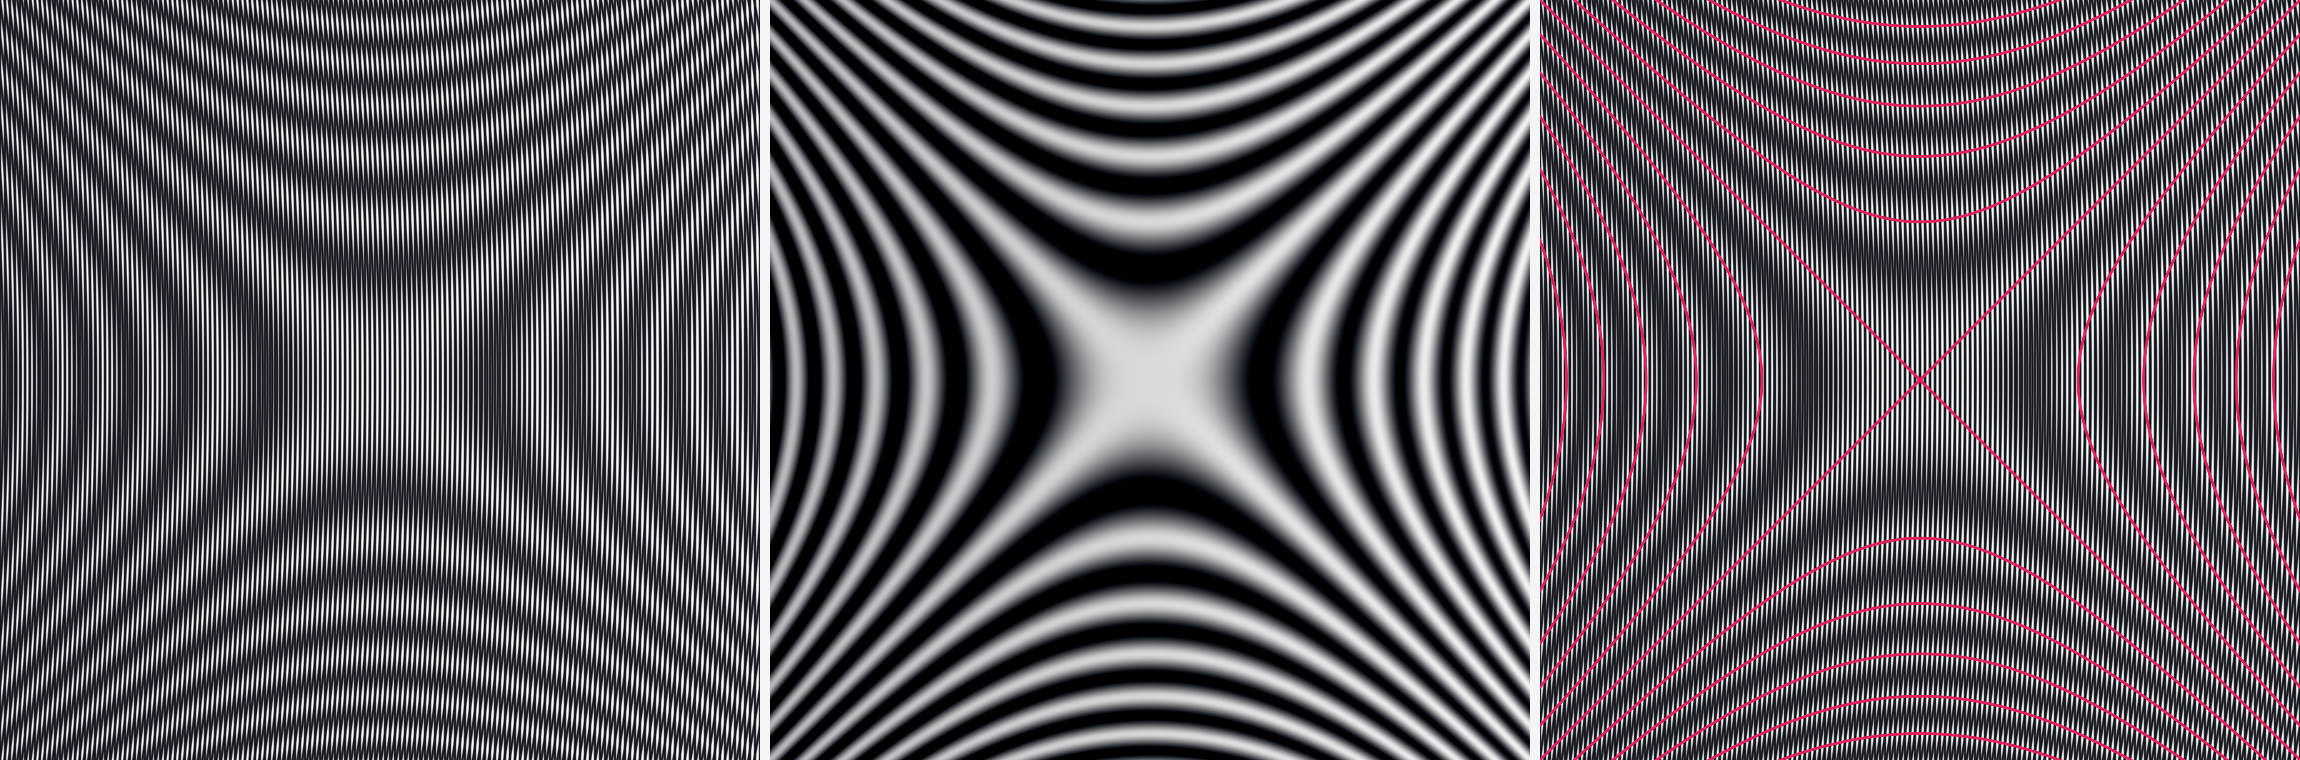
\includegraphics[width=\linewidth]{figures/contour-proof.png}
  \panelrow{0.33043}{0.00435}{%
    (a) as rendered,
    (b) envelope view,
    (c) with the true $\{f=nc\}$}
  \caption{\figlead{A contour plot that was never contoured.} \Moire{}'s
  \textsc{saddle} field encoded by \eqref{eq:encode} into a carrier of pitch
  $\contourCarrier$\,px. \textbf{(a)} The superposition, as rendered: two
  line families and nothing else. \textbf{(b)} The same two layers under the
  envelope view of \S\ref{sec:envelope}: the carrier is gone and the fringe field
  is what is left, its bright bands the level sets of the saddle. This is not a
  blur of (a); it is the mean ink of the same two fields, at the same resolution.
  \textbf{(c)} The rendered image again, with the true curves $\{f=nc\}$ drawn on
  top in pink. They are computed from $f$ alone and laid over a picture that never
  saw them. Note that $f=0$ is the asymptote pair, and the fringe field reproduces
  the crossing.}
  \label{fig:contourproof}
\end{figure*}

\subsection{Does the ink land on the curve?}

Theorem~\ref{thm:fringe} is a statement about a locally averaged quantity, so it
does not by itself promise that the visible bright band of a particular render is
centered on the mathematical curve. That is a question about a rasterized image
and it deserves a measurement rather than an argument.

We measure it as follows. Pick a point, walk it onto the nearest true level set
$\{f=nc\}$ by Newton steps along $\nabla f$ (exact, since \S\ref{sec:exprs}
differentiates every field as it evaluates it) and call the landing
point $q$. Low-pass the render along the carrier direction, enough to erase both
families' strokes and no more, so that nothing is smeared across the fringe we are
about to locate. Then sample that low-passed image along the contour normal
through $q$, fit a parabola to the three samples about the discrete maximum, and
read off the sub-pixel position of the peak. Its displacement from $q$ is the
error, in pixels.

The estimator has a bias of its own, so we calibrate it on a control whose answer
is known in advance, and we pick one that is itself a state of the tool: two
parallel families at pitches $\contourCarrier$ and $\contourDetune$, the oldest
moir\'e there is. Its difference is $x\,(1/s_1-1/s_2)$ exactly, so its fringes are
straight lines $\contourCtlGap$\,px apart. There the measured displacement is
$\contourFloor$\,px on average and $\contourFloorP$\,px at the $95$th percentile,
which is the floor of the method of measurement rather than of the method being
measured.

Against that floor, over $\contourProbes$ probes on the $\fieldCount$ presets of
Figure~\ref{fig:contourfields} (the expressions \Moire{} offers as starting
points, not a set chosen for the experiment), the mean displacement of the
fringe peak from the true contour is
$\contourBestErr$--$\contourWorstErr$\,px, with a worst $95$th percentile of
$\contourWorstP$\,px. That is the strongest statement this
experiment can support: the fringe is on the curve to within our ability to say
where the fringe is.

\begin{figure*}[t]
  \centering
  \Description{Two rows of six square panels. Each panel in the top row is cut
  corner to corner by a black-and-white dashed rule: above the cut is a fine
  black-on-white line texture, below it the same state with the texture gone and
  only broad smooth bands remaining. The six are a hyperbolic cross, two tight
  spiral nests side by side, three merging blobs, four ring nests in a square,
  concentric circles, and an irregular mottled texture. The bottom row shows the
  same six fields as smooth blue-to-yellow heat maps: a saddle, a dipole with one
  dark and one bright pole, three bumps, four vortices, a bullseye, and
  low-frequency noise. Each top panel's bands follow the contours of the map below
  it.}
  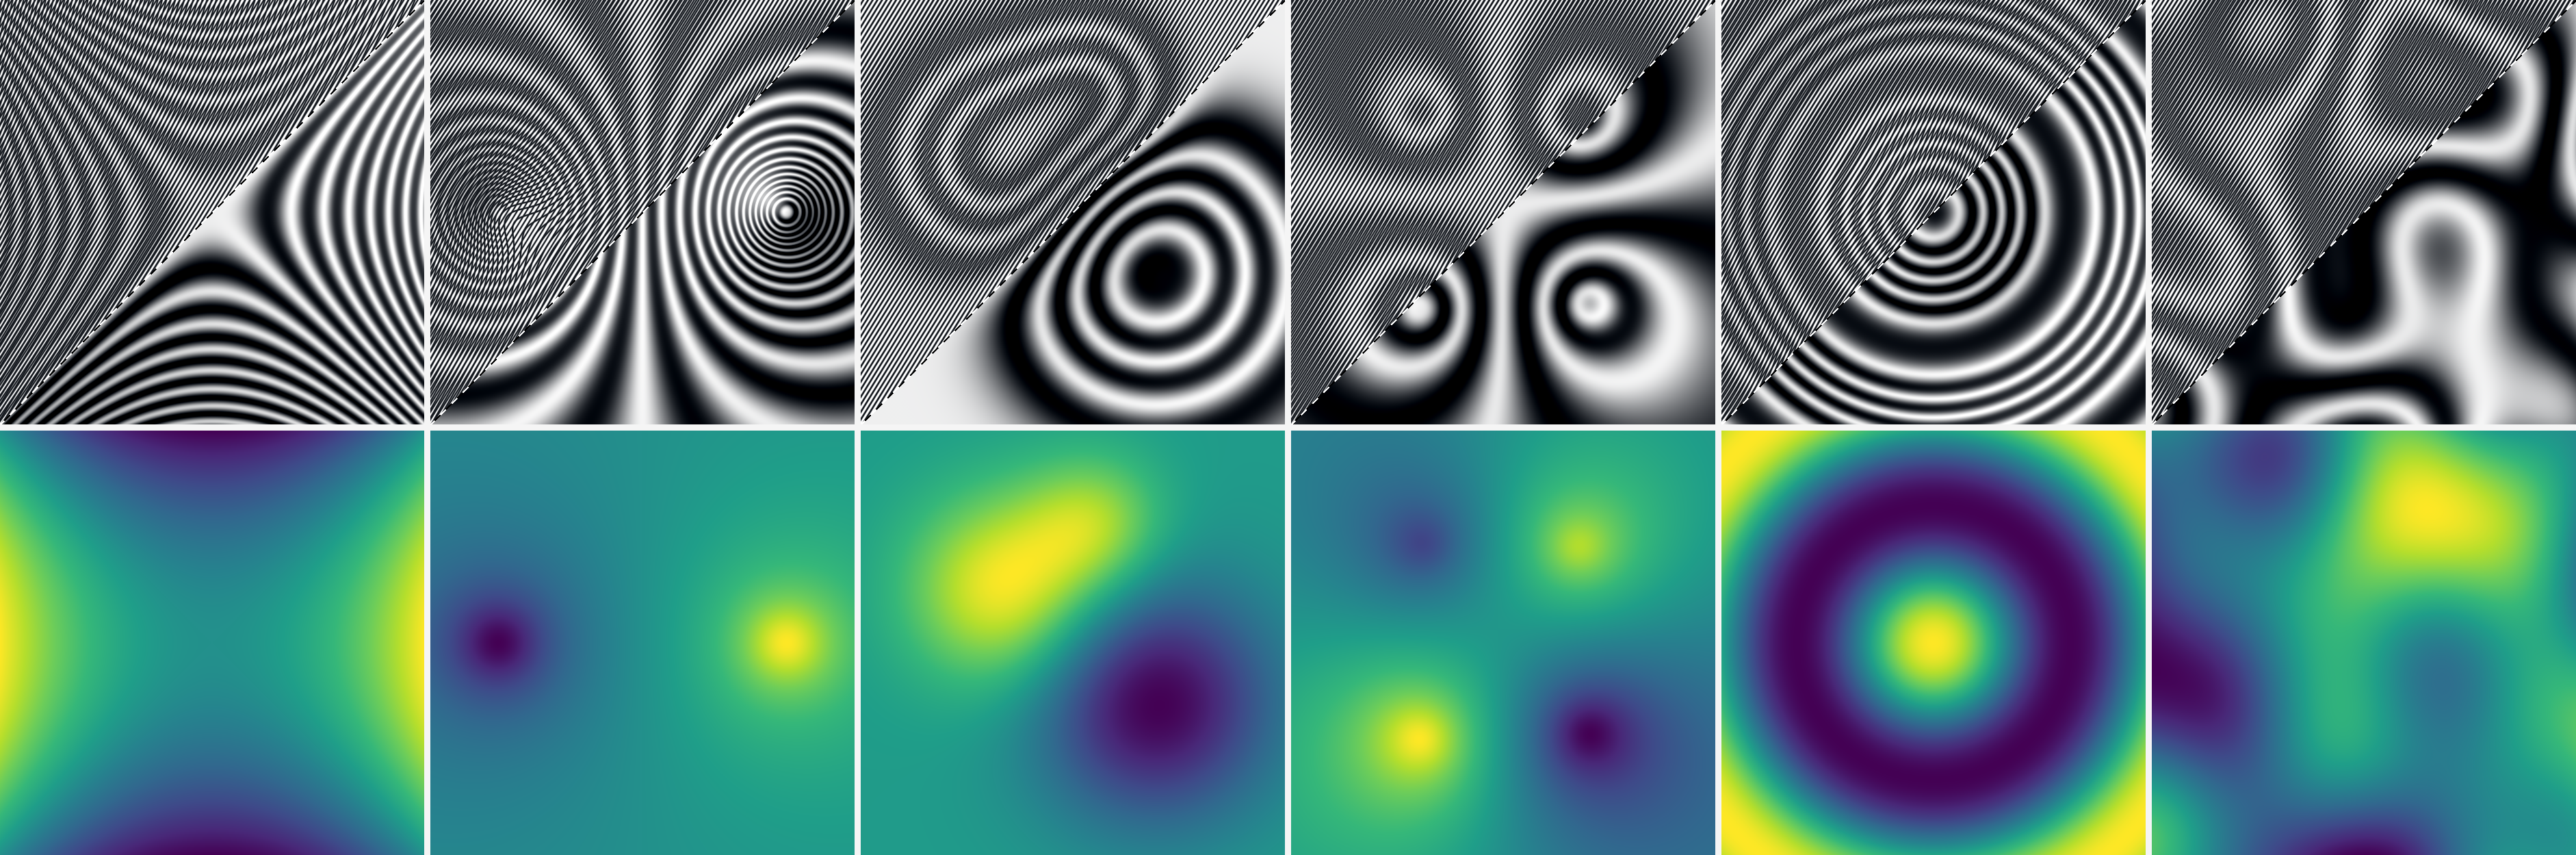
\includegraphics[width=\linewidth]{figures/contour-fields.png}
  \panelrow{0.16467}{0.00239}{%
    saddle, dipole, bumps, swirl, ripple, terrain}
  \caption{\figlead{Every preset the tool ships, encoded.} \emph{Top:} each panel
  is cut corner to corner: the superposition as rendered above the seam, the same
  two layers under the envelope view of \S\ref{sec:envelope} below it. The halves
  are two readings of one state, not two pictures: nothing is filtered between
  them, and the smooth side is the mean ink of the same two fields at the same
  resolution. \emph{Bottom:} the field each one encodes.
  Every pattern above is two \textsc{parallel} layers of pitch
  $\contourCarrier$\,px differing only in one layer's field expression; the labels
  are the presets of \S\ref{sec:exprs}, whose sources are in
  the supplemental material (\S S2). The dipole is instructive: towards each pole the
  equipotentials crowd, and past the limit \eqref{eq:contournyquist} no carrier can
  resolve them, so the render collapses into a dense scribble where the
  field is steepest, which reports the failure rather than hiding it. A contour tracer would emit dense
  polylines there without complaint.}
  \label{fig:contourfields}
\end{figure*}

\subsection{The sampling limit}

The interesting failure is visible in the dipole panel of
Figure~\ref{fig:contourfields}. Fringe spacing is $c/|\nabla f|$, so a field with
a steep region has contours that pack together, and a carrier of pitch $s$ cannot
carry a fringe much finer than itself. Empirically the fringe is legible while
\begin{equation}
  \frac{c}{|\nabla f|} \;\gtrsim\; 3s,
  \label{eq:contournyquist}
\end{equation}
and this is the whole of the method's sampling limit: one inequality, in local
quantities, both of which the renderer already has. It is a Nyquist statement
about the \emph{carrier}, not about the display, which is why raising the zoom
does not help but lowering $s$ does.

Two properties of \eqref{eq:contournyquist} are worth noting. First, it is a field, so it
can be drawn, as the heterodyne ratio of \S\ref{sec:visibility} can:
before committing to $c$, an author can be shown which parts of the frame will
resolve. Second, when it is violated the picture degrades \emph{loudly}. The
unresolvable region fills with visible high-frequency structure (the dipole's
poles turn into a black scribble), which is an honest report that the field is
steeper there than the chosen interval can show. A contour tracer, by contrast, returns a dense set of polylines with no
indication that the interval was too fine for the field.

\subsection{Other uses of the difference}

Equation~\eqref{eq:encode} is one line, and $f$ in it is arbitrary. Several things
follow that we have implemented but not studied, and we record them here
because the field formulation makes them cheap enough to be worth recording.

\paragraph{Streamlines.} A divergence-free planar flow has a stream function
$\Psi$ whose level sets are its streamlines. Encoding $\Psi$ by
\eqref{eq:encode} therefore draws the streamlines of the flow, with no
integration of trajectories, no seeding strategy, and no decision about how long
to trace before stopping. \Moire{}'s \textsc{swirl} field is the stream function
of four point vortices; encoding it draws closed streamlines around each vortex
and the separatrices between them, out of two \textsc{parallel} layers.

\paragraph{Two fields at once.} Two carriers, each with its own encoded partner,
give two independent differences, hence two fringe systems whose crossings are
the joint level sets $\{f=nc_f\}\cap\{g=mc_g\}$. We mention this
with a caveat, because it is where we found the ink budget binds: four dense
families in one frame drive the coverage towards saturation, and the two fringe
systems, though present and correct, are hard to see. Separating them by hue
helps and separating them by pitch helps more, but a clean two-field display
wants a compositing rule other than ``more strokes,'' and we do not have one.

\paragraph{Deformation, which is the classical case.} Let the second family be
the first pulled back through a map $T$, so $\ph_2=\ph_1\circ T$. Then
$D=(\ph_1-\ph_1\circ T)/s$, which to first order is $\langle \nabla\ph_1,
p-T(p)\rangle/s$: the component of the displacement along the family's gradient,
in units of the pitch. The fringes are its contours. This is precisely what
shadow moir\'e, moir\'e topography and moir\'e deflectometry measure with physical
gratings~\cite{Post1994High, Post2008Moire, Takasaki1970Moire}, and it falls out of
\eqref{eq:contourlaw} as the special case $f=\ph_1-\ph_1\circ T$. We note it not
as a new result but as a sanity check on the formulation: the oldest quantitative
use of moir\'e is a corollary of the fringe law, and the amplification factor those
instruments are prized for is the $1/s$ in front. Nothing special is needed to get
it: a vertical carrier and the \textsc{bumps} field is a grating photographed
against its own shadow on a bumpy surface.

\paragraph{Error and disagreement.} Nothing requires $f$ to be a physical field.
Encoding the difference between an approximation and a reference makes the
fringes the contours of the error, at an interval the author sets, in a display
whose ink is legible at any zoom. We found this useful while
debugging the renderer in this paper.

None of this is a new measurement principle; interferometry has used fringe
counting for a century. What is new is where it now sits. These are two extra
terms in a shader in a drawing tool, they run at frame rate, they compose with the
\patternCount{} families of \S\ref{sec:catalog} and with each other, and the
picture they make is a picture---something an author can restyle, zoom, and
put on a page---rather than the output of a measurement pipeline.

\section{Discussion}
\label{sec:discussion}

\paragraph{What generalizes.}
Nothing in Sections~\ref{sec:drift}--\ref{sec:skip} used two dimensions, and
nothing used regular polygons beyond the value of $\kappa$. The argument needs
exactly four things: a metric that is a support function of some convex body
inside the unit ball, a lower bound $\kappa\lVert q\rVert$ on it, an index-affine
motion of the frames, and a renderer that clamps the field at a known guard. Any
family of nested convex level sets under a one-parameter rigid motion admits the
same interval, with $\kappa$ the inradius of the normal hull and
$m=\rad(-\delta)$ the support value along the walk. In $3$D the same construction
covers nested convex shells under a screw motion; $\kappa$ becomes the inradius of
the normal hull of the polyhedron, and Proposition~\ref{prop:closed} becomes a max
over faces rather than edges. We have not implemented this, but the proofs do not
change.

Conversely, the method fails cleanly where the hypotheses fail. A non-convex
generator has no support-function representation, so (P2) and (P4) go and with them
the interval and the closed form; the Lipschitz skip survives, since it needs only
(P1). A motion that is not affine in the index (rings whose rotation
accelerates, say) loses the affine envelopes but keeps a Lipschitz bound if the
motion is Lipschitz in $n$, so Algorithm~\ref{alg:scan} would still run, only
without a certificate.

\paragraph{Why the discrete setting is favorable.}
Why does this problem admit a stronger guarantee than the
continuous analogues in Section~\ref{sec:related}? Range analysis on a spatial
domain must subdivide, because the domain is uncountable and the bound is
conservative; it terminates on a tolerance. Here the domain is $\N_0$, the interval
is exact rather than conservative, and ``enumerate the interval'' is a terminating
algorithm that returns the true minimum, not an approximation of it. Discreteness
converts a tolerance into a proof. We suspect other rendering problems phrased as
``which member of this indexed family is nearest'' (glints~\cite{Yan2014,
Yan2016}, tiled or stamped patterns~\cite{Lagae2010}, layered fibers) have the
same structure available and are being solved with budgets instead.

\paragraph{What the representation provided, besides speed.}
We began with the field formulation as a way to get resolution independence, and
that is what it delivered. What we did not expect is that it would function as a
debugging method. Four shipped bugs were found the same way, by writing the
layer's definition down and watching a unit fail to agree: the missing eikonal
divide (\S\ref{sec:eikonal}; supplemental \S S2), a stroke floor applied in
phase units, a subsampling anchor nobody had noticed was a choice
(\S\ref{sec:results}), and an envelope pivot that counted a hex lattice as one
family when it draws three (\S\ref{sec:envelope}). A representation that names
the quantities forces the units to agree, and most of our bugs were units. It
also says which quantities must never be written twice. Each of our first six
fields carried a gradient derived by hand and transcribed into two languages;
the definition of a layer says that gradient is a consequence of the field, not
an attribute of it, and forward-mode differentiation (\S\ref{sec:exprs}) removes
the transcriptions along with the class of bug they were the only source of.

\paragraph{Where the ink runs out.}
The formulation's real budget is not arithmetic, it is coverage. A layer costs one
distance query, so twelve layers cost twelve; but twelve dense families of ink in
one frame is a black rectangle, and the pattern is gone long before the frame rate
is. This bound binds in exactly one place we wanted to go: displaying two encoded
fields at once (\S\ref{sec:beyond}) needs four families, and four families of
strokes at a pitch fine enough to carry fringes saturates. Hue and pitch separation
help and are not enough. We think the missing piece is a compositing rule for
fields that is not union-of-ink, something that spends contrast rather than
coverage, and we do not have one. Of the open problems in this paper it is the one that matters most, because it
is what stands between a moir\'e and a display with more than one channel.

\paragraph{Limitations.}
Five, in decreasing order of severity. \emph{The scan's reach follows its
gradients.} The selection of \S\ref{sec:selection} is order-free only where
both index gradients are closed-form; a walking family's gradient is a
screen-space difference, whose per-quad noise the reduction reads as slow
high-order characters, so a pair involving one keeps the old order-two floor,
and a lattice's candidate combinations are still an enumeration (the first
three dual rings, supplemental \S S3), so a sufficiently extreme lattice pair
can beat outside them. Both caps are now exceptions that name their cause
rather than a ceiling on the theory.
\emph{The marginal band.} On
$\rad(-\delta)=s$ with $\theta\neq0$ the interval is genuinely infinite and we
neither enumerate it nor prefilter it; we subsample, coherently, and accept up to
$\degLegibleWorst\%$ ink loss in the legible corner of that band
(Section~\ref{sec:limits}). Proposition~\ref{prop:closed} solves the $\theta=0$
slice exactly, which suggests the rotated case is not hopeless: the residual there
is a sinusoid plus a line, and the indices where it can vanish are governed by the
continued-fraction expansion of $\theta/2\pi$: the same arithmetic
\S\ref{sec:selection} made the criterion's, so the tools are already in the
renderer. We consider it the most promising follow-on. \emph{The metric.} We minimize the residual of the inradius metric, not
Euclidean distance to the curve, which thickens strokes near polygon corners by up
to $1/\kappa$; dividing by $\lVert\nabla\rad\rVert$ would fix it, at the cost of
the exact envelopes. \emph{Prefiltering.} We show the wide-interval regime is
saturated but do not integrate the field there; a correct analytic mean over a
walking family is open, and would replace the subsampling fallback with something
principled rather than merely coherent. \emph{Families without a scalar index.}
Four of our thirteen (the radial pencil and the three lattices) have no
phase function in the sense of \S\ref{sec:catalog}: the pencil's index is an angle, so its fringes
are not level sets of a difference of scalars, and a lattice's index is a pair of
integers, so a lattice pair produces a two-dimensional beat that the fringe law
describes only along a chosen direction. They render correctly, and both are
classical enough that the beat is well understood elsewhere
\cite{Amidror2009Theory,Oster1964}; they simply sit outside the theorem, and a
vector-valued index law that covered them would be a genuine extension.

\paragraph{Future work.}
\label{sec:future}
Beyond the marginal band and prefiltering: the interval is computed per pixel from
$r$, $\Lambda$, and $\kappa$, all of which vary smoothly, so a conservative
interval could be computed once per tile and shared, which on a GPU trades
divergence for a slightly wider scan, probably a win at zoom-out given the
divergence measurements in Table~\ref{tab:ablation}. And since the residual's
zero set is a curve in $(p, n)$ space, a screen-space continuation that carried
$n^\star$ from pixel to pixel would reduce the search to a local refinement almost
everywhere, with the interval available as the certificate that reseeds it when the
continuation breaks.

\section{Conclusion}

Moir\'e has been drawn the same way for a century and a half: put down two layers
of marks and let the overlap do the rest. Drawn that way, the fringe is an
accident of sampling: what the overlap happened to produce, rather than what
was asked for. We have argued that a moir\'e layer is better described by two
scalar fields, an index and a distance, and that with those in hand the fringes
stop being an accident. They are the unit level sets of the difference of the
index fields (Theorem~\ref{thm:fringe}), a statement that under its local
hypotheses needs no periodicity, no lattice, and no Fourier transform, and that
we measured holding on every family we tested, including one whose index
field exists only as the answer to a search.

Three things follow. The pattern becomes a document rather than a raster:
resolution-independent, so that one description is a thumbnail, a screen, and a
plate. The fringe becomes predictable before it is drawn, because the local
ratios $\het_k$ of Eq.~\ref{eq:ratiok} say where one will appear and how it
will run, and \emph{which} beat it will be is no longer scanned for but
computed: the visible-beat hierarchy is the continued fraction of the local
pitch ratio, found at any order by per-pixel lattice reduction
(\S\ref{sec:selection}), so the classical order cap is deleted rather than
raised. And the fringe becomes \emph{addressable}:
choosing the index fields so that their difference is a field of interest turns
the moir\'e into a contour plot of that field, which we verified localizes to a
mean of $\contourWorstErr$\,px against ground truth on the hardest of
\contourFieldCount{} fields, written as expressions and differentiated as they
are evaluated so that a field the author invents arrives with the gradient the
renderer requires; a circle-valued field ends fringes at defects whose signed
endings count its winding exactly (\S\ref{sec:defects}).

Making this run at interactive rates cost the paper's other half. When each member
of a family carries its own rigid motion there is no global index field, and the
per-pixel question becomes an inversion over the integers. We showed that one
classical object, the support function of the generating shape, supplies
everything needed to replace the usual fixed-window guess with a certificate: a
Lipschitz modulus, an exact anisotropy floor $\cos(\pi/N)$, an exact drift rate
$\rad(-\delta)$, and, when the per-index rotation vanishes, convexity of the
residual and hence an exact solution for polygons of any side count, including the
marginal case where no finite enumeration can succeed. That is
$\gpuSpeedLo$--$\gpuSpeedHi\times$ faster than the enumeration it replaces
across rotated settings, and in exact agreement with brute force on every
legible setting of the fidelity sweep (\S\ref{sec:limits} measures the strided
band the sweep's cap excludes).

The work is embodied in \Moire{}, a browser tool in which thirteen families,
twelve simultaneous layers, authored fields, and every parameter in this paper
are live under the cursor at $60$\,Hz. Building it is what produced the
mathematics: the eikonal divide, the pixel-relative stroke floor, and the drift
interval were each found by dragging a slider until something looked wrong. A
field formulation is a good way to make a pattern precise, but an instrument
that moves is a good way to find out which parts of it are false.

Two lessons we would carry elsewhere. A bound that is merely loose, not wrong, can
still produce a visibly broken image whenever the fallback for a loose bound is
approximation, so the tightness of a constant is not always a performance
question. And when approximation is unavoidable, its structure matters more than
its magnitude: the same missing ink reads as a thinner pattern or a shattered one
depending only on whether the samples are anchored to the family or to the pixel.


\bibliographystyle{ACM-Reference-Format}
\bibliography{refs}

\appendix
\section{Proofs}
\label{app:proofs}

\subsection{The fringe law}
\label{app:fringe}

\begin{proof}[Proof of Theorem~\ref{thm:fringe}]
Recall the setting. Layer $i$ has index field
$\idx_i$, and its ink at a point $q$ comes from thresholding the Euclidean distance
to the nearest member,
\begin{equation}
  d_i(q)=\frac{\mathrm{pd}\big(\idx_i(q),1\big)}{\lVert\nabla\idx_i(q)\rVert},
  \label{eq:appdist}
\end{equation}
against the half-width $h_i$ with an antialiasing band $a$, giving
$\alpha_i(q)=1-\mathrm{smoothstep}(h_i-a,\,h_i+a,\,d_i(q))$. Here
$\mathrm{pd}(x,1)=\min_{n\in\Z}\lvert x-n\rvert$ is the distance to the nearest
integer. The two layers share a color and composite as a union,
$\alpha=\alpha_1+\alpha_2-\alpha_1\alpha_2$.

\paragraph{Step 1: move the threshold into index units.}
Substituting \eqref{eq:appdist}, the condition $d_i\le h_i$ is
$\mathrm{pd}(\idx_i,1)\le h_i\lVert\nabla\idx_i\rVert$. Writing
$w_i=h_i\lVert\nabla\idx_i\rVert$ and $b_i=a\lVert\nabla\idx_i\rVert$ for the
half-width and band \emph{measured in index units}, and
\begin{equation}
  A_i(v)=1-\mathrm{smoothstep}\big(w_i-b_i,\;w_i+b_i,\;\mathrm{pd}(v,1)\big),
  \label{eq:appprofile}
\end{equation}
we have exactly $\alpha_i(q)=A_i(\idx_i(q))$. This is the only place the eikonal
factor of \S\ref{sec:eikonal} is used, and it is used twice: once to make the
threshold comparable to a length, and once to make $w_i$ and $b_i$ constants
rather than functions of $q$, which is where the theorem's constant-gradient
hypothesis enters, and why it cannot be dropped. The verification in
\S\ref{sec:fringe} excludes samples whose gradient varies by more than $15\%$
across a period for exactly this reason.

\paragraph{Step 2: reparameterize the segment by index.}
Let $g=\tfrac12(\nabla\idx_1+\nabla\idx_2)$, let $u=g/\lVert g\rVert$, let
$T=1/\lVert g\rVert$, and parameterize $S$ by arclength $t\in[-T/2,T/2]$, so
$q(t)=p+tu$. With $\nabla\idx_1$ constant on $S$, the map $t\mapsto
v=\idx_1(q(t))$ is affine with slope $\langle\nabla\idx_1,u\rangle$, hence a
measure-preserving reparameterization onto an interval of length
\begin{equation}
  \langle\nabla\idx_1,u\rangle\,T
  \;=\;\frac{\langle\nabla\idx_1,u\rangle}{\lVert g\rVert}
  \;=\;1+\tfrac12\,\frac{\langle\nabla D,u\rangle}{\lVert g\rVert}
  \;=\;1+O(\het),
\end{equation}
since $\nabla\idx_1=g+\tfrac12\nabla D$ and $\het=\lVert\nabla D\rVert/\lVert
g\rVert$; when $D$ is constant on $S$ the middle term vanishes and the length is
exactly $1$. So averaging over $S$ in $t$ is averaging over one unit period in
$v$, exactly in the constant case and to first order in $\het$ otherwise; and
because both $A_1$ and $A_2$ are $1$-periodic, the choice of representative
period does not matter.

\paragraph{Step 3: the constant case.}
By definition $\idx_2=\idx_1-D$, so in the new variable the second layer's
argument is $v-D$. If $D$ is constant on $S$, equal to $D(p)$, then
\begin{align}
  \bar\alpha(p)
  &=\int_0^1\Big[A_1(v)+A_2\big(v-D(p)\big)-A_1(v)A_2\big(v-D(p)\big)\Big]\mathrm{d}v
  \notag\\
  &=\Phi\big(D(p)\big),
\end{align}
which is \eqref{eq:phi}. Every dependence on $p$ has been absorbed into the single
number $D(p)$: the individual index fields have disappeared, and with them any
notion of periodicity, orientation, or curvature of either family. This is the
content of the theorem.

% Declared here rather than beside the sentence that discusses it. A figure* can
% only be set at the top of a page, and read at its reference this one had no page
% top left to reach: it fell past the end of the appendix onto a page of its own.
\begin{figure*}[t]
  \centering
  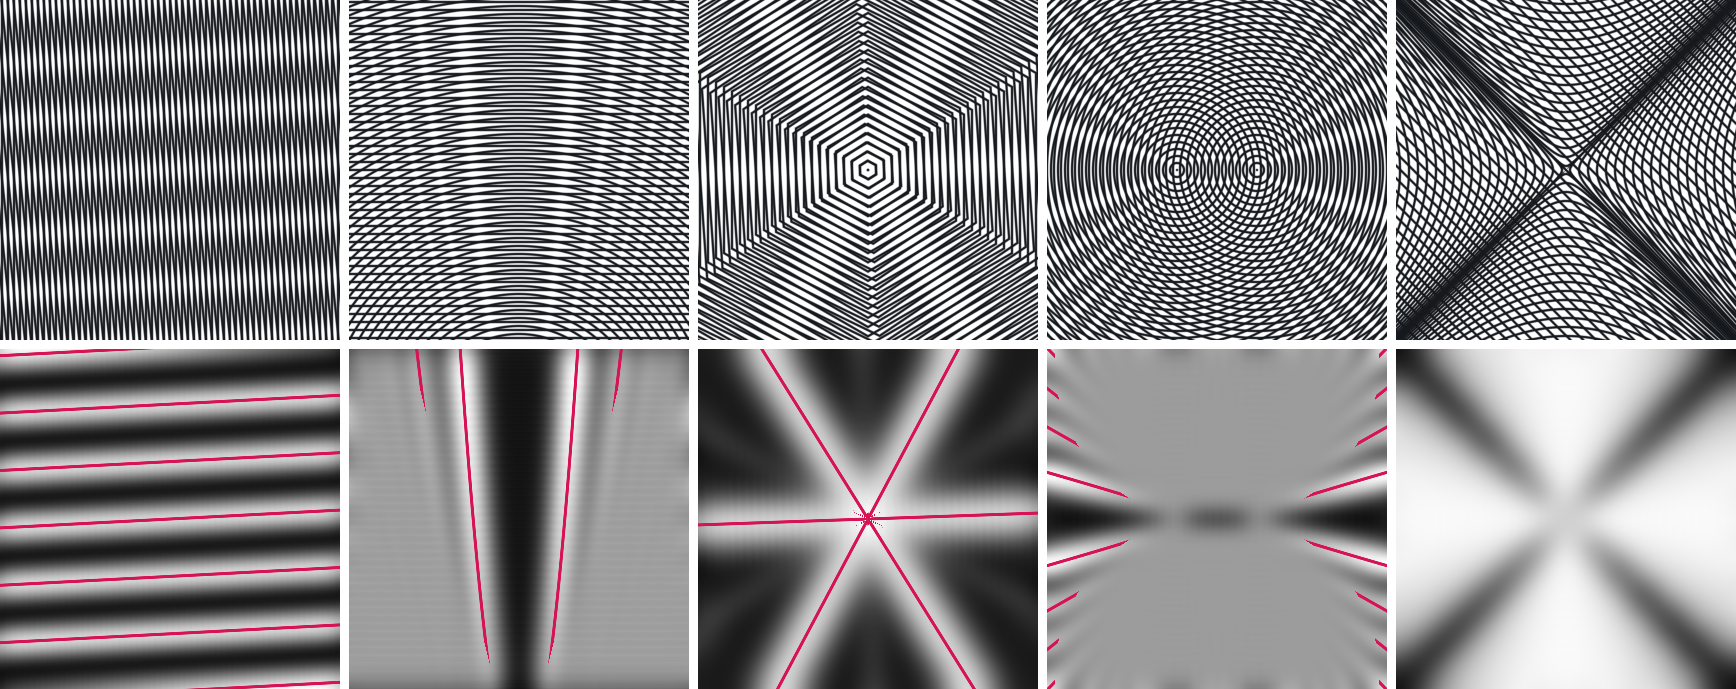
\includegraphics[width=\textwidth]{figures/law-atlas.png}
  \panelrow{0.19576}{0.00530}{%
    (a) two combs,
    (b) circles under lines,
    {(c) hexagons, $4^\circ$},
    {(d) circles, two centers},
    (e) hyperbolae under lines}
  \Description{Two rows of five square panels. The top row shows five moire
  superpositions: two nearly parallel line combs; concentric circles crossed by
  slanted lines; two hexagon families four degrees apart; two circle families with
  displaced centers; and rectangular hyperbolae under slanted lines. The bottom row
  shows the same five frames blurred to gray fringe fields, with crimson curves drawn
  on the light fringes. The crimson curves cover the whole panel in the first, are
  confined to a wedge at one side in the second, radiate as six rays in the third,
  appear only along the top and bottom in the fourth, and in the fifth trace two
  short arcs inside an otherwise refused frame.}
  \caption{\figlead{The law and the criterion, across the catalog.} \emph{Top:} five
  of the pairs measured in Table~\ref{tab:fringe}, rendered from their distance
  fields. \emph{Bottom:} each frame low-passed to its fringe field, with the unit
  level sets of the \emph{winning} character over it in crimson, drawn only where
  the weighted merit $\mu_k\le1/4$ (\S\ref{sec:selection}) and fading out over the
  last tenth of that range, so a curve ending
  is the criterion's edge and not the pixel grid's. Ordered by the fraction of the frame the criterion admits: $\atlasCombs\%$,
  $\atlasCircleLines\%$, $\atlasHex\%$, $\atlasCircles\%$, $\atlasControl\%$.
Column~(b) is masked to a wedge, outside which the circles and the lines cross at
a wide angle; (d) near its two centers, where the superposition is a rosette and
not a fringe field at all. Column~(e) is the instructive one: the first-order
criterion refuses this frame outright (Table~\ref{tab:fringe}'s last row has no
in-regime samples), the bright corridor along the asymptotes belongs to the
hyperbola family alone, and the $\atlasControl\%$ the order-free scan still
admits is a pair of commensurate pockets where a higher-order character locks
onto the hyperbolae, the same stations Figure~\ref{fig:selection}a resolves.
Curves are also suppressed wherever consecutive level
  sets fall closer together than they can be drawn apart: at the center of (c)
  the difference is singular and its level sets crowd without bound, so anything
  drawn there would be speckle rather than a curve. The curves come from the two
  index fields and the mask from their gradients, so the whole bottom row costs two
  gradients per pixel and reads no raster, which is why the tool can tell a user
  that a pair of layers will not interfere before it draws them.}
  \label{fig:lawatlas}
\end{figure*}

\paragraph{Step 4: the hard-edged limit.}
Let $b_i\to0$, so $A_i$ becomes the indicator of
$\{\mathrm{pd}(v,1)\le w_i\}$, an interval of length $2w_i$ per period. Then
$\int_0^1 A_i=2w_i$, and $\int_0^1A_1(v)A_2(v-\Delta)\,\mathrm{d}v$ is the
overlap of two arcs of half-widths $w_1$ and $w_2$ whose centers are
$t=\mathrm{pd}(\Delta,1)$ apart. That overlap is $w_1+w_2-t$ only while the arcs
partially overlap; once one lies inside the other ($t\le|w_1-w_2|$) it saturates
at $2\min(w_1,w_2)$, and once they separate it is zero, so
$\mathrm{overlap}=\min\big(2\min(w_1,w_2),\,\max(0,\,w_1+w_2-t)\big)$. A second
overlap across the far side of the period would need $w_1+w_2>1-t\ge\tfrac12$,
which the theorem's hypothesis $w_1+w_2\le\tfrac12$ excludes; this is where
that hypothesis is used, and without it \eqref{eq:tent} overcounts (the integral
form \eqref{eq:phi} does not). Hence
\begin{equation}
  \Phi(\Delta)=2w_1+2w_2-\min\!\big(2\min(w_1,w_2),\;\max\big(0,\;w_1+w_2-t\big)\big),
\end{equation}
which is \eqref{eq:tent}. It is piecewise linear in $t$, with slope $0$ while one
stroke lies inside the other, slope $1$ while they partially overlap, and slope $0$
after they separate: a tent with a flat floor and a flat top, minimized at
$\Delta\in\Z$ at the value $2\max(w_1,w_2)$ and maximized at $2w_1+2w_2$ wherever
$t\ge w_1+w_2$. Note that the plateau is reached strictly inside the period
whenever $w_1+w_2<\tfrac12$, which is the regime the tool operates in and the
reason thickening strokes eventually stops changing the fringe.

\paragraph{Step 5: the non-constant case, and why the error is first order.}
Suppose now that $D$ varies on $S$; with the gradients constant it is affine
there. In the index variable write $D=D(p)+\mu\,(v-v_p)$, where $\mu$ is the
change in $D$ per unit index, so that
$\lvert\mu\rvert\le\het+O(\het^2)$ by the definition of $\het$ (with equality
when $\nabla D$ is parallel to $u$). Put
$F(v,\Delta)=A_1(v)+A_2(v-\Delta)-A_1(v)A_2(v-\Delta)$, so that
$\Phi(\Delta)=\int_0^1F(v,\Delta)\,\mathrm{d}v$. Averaging over the period and
expanding in $\mu$,
\begin{equation}
  \bar\alpha(p)=\Phi\big(D(p)\big)
  +\mu\int_{-1/2}^{1/2}\!\! (v-v_p)\,\partial_\Delta F\big(v,D(p)\big)\,\mathrm{d}v
  +O(\mu^2).
  \label{eq:appfirst}
\end{equation}
The integral is bounded: $\partial_\Delta F(v,\Delta)=A_2'(v-\Delta)\,(A_1(v)-1)$,
$\lvert v-v_p\rvert\le\tfrac12$ on the period, $\lvert A_1-1\rvert\le1$, and
$\int_0^1\lvert A_2'\rvert\le2$ for the single-bump profile \eqref{eq:appprofile},
so the correction is at most $\lvert\mu\rvert$ in absolute value. Hence
$\bar\alpha(p)=\Phi(D(p))+O(\het)$, as claimed.
\end{proof}

\begin{remark}
The first-order term does not vanish identically. It is odd in
$(v-v_p)$ against a factor that is not even, so no symmetry argument kills it,
and one should expect a genuine $O(\het)$ perturbation of the profile: a
slight asymmetry leaning in the direction the carrier is changing. Its effect
on the \emph{positions} of the extrema depends also on the profile's curvature
there, and on a plateaued extremum the position is not $O(\het)$-stable at all;
the measured statistic is consistent with this: the light fringes of
Table~\ref{tab:fringe} sit at mean index gap $\fringeLight$ from an integer
rather than at $0$, a fraction of the regime bound $\het=1/4$.
\end{remark}

Figure~\ref{fig:lawatlas} is the theorem and its hypothesis drawn together, on five
of the pairs Table~\ref{tab:fringe} measures.

\paragraph{The remaining proofs.} Each bound of \S\ref{sec:inverse} is short and is
proved where it is stated: the drift constant in \S\ref{sec:drift}, the two-sided
envelope as Lemma~\ref{lem:envelope}, the sufficient interval as
Theorem~\ref{thm:window}, the Lipschitz skip as Lemma~\ref{lem:lipschitz}, the
translated-polygon closed form as Proposition~\ref{prop:closed}. The fold law
and its consequences are proved below.

\subsection{The fold law and the reach of closed forms}
\label{app:foldlaw}

\begin{proof}[Proof of Lemma~\ref{lem:foldlaw}]
For a convex body with $C^2$ support function $H_n$, the boundary is
parameterized over contact angles by
$x(u,n)=H_n(u)\,\hat u+H_n'(u)\,\hat u^{\perp}$, with
$\hat u=(\cos u,\sin u)$ and $\hat u^{\perp}=(-\sin u,\cos u)$; this is the
standard support parameterization~\cite{Schneider2014Convex}. Differentiating,
and using $\hat u'=\hat u^{\perp}$, $(\hat u^{\perp})'=-\hat u$,
\begin{equation*}
  \frac{\partial x}{\partial u}=(H_n+H_n'')\,\hat u^{\perp},
  \qquad
  \frac{\partial x}{\partial n}
    =(\partial_nH_n)\,\hat u+(\partial_nH_n')\,\hat u^{\perp},
\end{equation*}
so $\det[\partial_ux,\ \partial_nx]
=(H_n+H_n'')\,(\partial_nH_n)\,\det[\hat u^{\perp},\hat u]
=-(H_n+H_n'')\,\partial_nH_n$. The factor $H_n+H_n''$ is the curvature radius
of the member, nonnegative by convexity, so away from the corner set the
member map is singular --- the family has an envelope, its fold --- exactly
where $\partial_nH_n=0$. Differentiating \eqref{eq:famsupport} in $n$ gives
\eqref{eq:foldlaw}. A polygon's $H$ is piecewise trigonometric with corners
at the vertex directions; the lemma applies on each smooth arc, the one-sided
derivatives at a corner are the two adjacent facets' endpoints (the body's
vertices), and the suprema below are attained there.
\end{proof}

\begin{proof}[Proof of Corollary~\ref{cor:rotation}]
With $\delta=0$, \eqref{eq:foldlaw} reads $sH(w)=\rho_n\theta H'(w)$, i.e.
$\rho_n=s/(\theta\cdot H'(w)/H(w))$, solvable at the smallest gauge radius
$\rho^\star=s/(\theta L)$ with $L=\sup_w|H'/H|$ (the catalog's gauges are
symmetric, so the sup is attained with either sign). For the regular $k$-gon
of unit inradius, $H(u)=\sec(\pi/k)\cos(\tilde u)$ on each arc, where
$\tilde u\in[-\pi/k,\pi/k]$ is the offset from the nearest vertex direction;
$|(\log H)'|=|\tan\tilde u|\le\tan(\pi/k)$, attained at the arc ends. There
$H=1$, $H'=\mp\tan(\pi/k)$, and the fold point
$x=\rho(H\hat u+H'\hat u^{\perp})$ has
$\lVert x\rVert=\rho\sqrt{1+\tan^2(\pi/k)}=\rho\sec(\pi/k)$: the vertex, at
Euclidean radius $R^\star=\rho^\star\sec(\pi/k)=s/(\theta\sin(\pi/k))$. For
the ellipse gauge, $H(u)=\sqrt{a^2\cos^2u+b^2\sin^2u}$; writing
$A=(a^2+b^2)/2$, $B=(a^2-b^2)/2$, we have $H^2=A+B\cos2u$ and
$(\log H)'=-B\sin2u/H^2$, maximized at $\cos2u^\star=-B/A$ with value
$B/\sqrt{A^2-B^2}=(a^2-b^2)/2ab=L$. At $u^\star$, $H^2=a^2b^2/A$ and
$H'^2=B^2/A$, so
$\lVert x\rVert=\rho\sqrt{H^2+H'^2}=\rho\sqrt{(a^2b^2+B^2)/A}=\rho\sqrt{A}$,
since $a^2b^2+B^2=A^2$: the stated $R^\star=\rho^\star\sqrt{(a^2+b^2)/2}$.
Finally $L=0$ iff $H'\equiv0$ iff $H$ is constant iff $K$ is a centered
disc, so the circle is the unique rotation-immune gauge.
\end{proof}

\begin{proof}[Proof of Corollary~\ref{cor:mach}]
With $\theta=0$, $\partial_nH_n(u)=sH(u)+\langle\delta,\hat u\rangle$, which
is negative somewhere iff
$\sup_u\langle-\delta,\hat u\rangle/H(u)>s$. That supremum is the gauge:
$x\in tK$ iff $\langle x,\hat u\rangle\le tH(u)$ for all $u$, so
$\sup_u\langle x,\hat u\rangle/H(u)=\rad(x)$, and the fold condition is
$\rad(-\delta)>s$, uniform in $n$ (hence ``immediately''). At a critical
angle $u^\star$ the envelope points
$x(u^\star,n)=H_n(u^\star)\hat u^\star+H_n'(u^\star)\hat u^{\star\perp}$ are
affine in $n$: straight wake lines. For circles ($H\equiv1$) the critical
directions are the unit vectors $\nu$ with
$\langle\delta,\nu\rangle=-s$, and
$\langle x,\nu\rangle=H_n(u^\star)=ns+\varphi+n\langle\delta,\nu\rangle=\varphi$:
the tangent pair. With rotation, $c(n)=\Rot{n\theta}(n\delta)$ gives
$c'(n)=\Rot{n\theta}\delta+n\theta\,\Rot{n\theta+\pi/2}\delta$, two orthogonal
components of lengths $\lVert\delta\rVert$ and $n\theta\lVert\delta\rVert$,
so $\lVert c'(n)\rVert=\lVert\delta\rVert\sqrt{1+n^2\theta^2}$, and for
circles the condition $\lVert c'(n)\rVert>s$ first holds at
$n^\star=\sqrt{(s/\lVert\delta\rVert)^2-1}/\theta$.
\end{proof}

\begin{proof}[Proof of Proposition~\ref{prop:untwist}]
Rational case: with $\theta=2\pi a/b$ and $n=j+bk$,
$n\theta\equiv j\theta\pmod{2\pi}$, so on the class the pulled-back point is
$\Rot{-j\theta}p-n\delta$: a fixed rotation of $p$ minus an affine walk. The
residual is a convex gauge of an affine path, hence convex in $n$ on the
class; for the circle gauge,
$\lVert\Rot{-j\theta}p-n\delta\rVert=\lVert p-n\Rot{j\theta}\delta\rVert$,
and squaring the incidence gives one quadratic per class. The frames
$\{n\theta\bmod2\pi\}$ form a finite set iff $\theta/2\pi\in\Q$ (a subgroup
of the circle is finite or dense), so no such split exists otherwise.

Transcendence: suppose the interpolated incidence
$I=\{(p,\nu):\lVert p-c(\nu)\rVert=\nu s+\varphi\}$ were semialgebraic for
some $\theta\neq0$. Each slice $I_\nu$ is a circle of positive radius, and
the center of a circle is first-order definable from the circle over the
real field, so $\nu\mapsto c(\nu)$ would be a semialgebraic function; its
first coordinate $f(\nu)=\nu\lVert\delta\rVert\cos(\nu\theta+\beta)$ would
satisfy $P(\nu,f(\nu))\equiv0$ for some nonzero polynomial
$P(\nu,y)=\sum_{j\le d}q_j(\nu)y^j$ with $q_d\not\equiv0$. Extend to complex
$\nu=it$, $t\to\infty$: $|\cos(it\theta+\beta)|$ grows like
$e^{\theta t}/2$, so the term $q_j(\nu)f(\nu)^j$ grows like
$e^{j\theta t}$ times a polynomial in $t$. The orders are distinct, so the
identity forces $q_d\equiv0$, a contradiction. (For a polygon or ellipse
gauge the same argument runs through the frame angle, definable from a slice
by its vertex or axis directions.)
\end{proof}

\paragraph{Group families never fold.} The claim of \S\ref{sec:taxonomy}:
if $\gamma_0$ crosses each orbit of the flow $\{g^t\}$ exactly once,
transversally, then $(u,t)\mapsto g^t(\gamma_0(u))$ is a bijection onto the
swept region with everywhere-invertible differential (transversality is
preserved because each $g^t$ is a diffeomorphism), so the family
$\{g^n\gamma_0\}$ is a foliation and the index --- the $t$-component of the
inverse --- is a submersion: no envelope can form. A rotational flow's clock
gains its period on each circuit of the fixed point, and the gain counts the
members a circuit crosses, which is the winding rung's quantized charge;
flows without a rotational part have proper orbits and a single-valued
clock.


\end{document}
